%!TEX encoding = UTF-8 Unicode
\documentclass{ctexart}
\usepackage{color}
\usepackage{xcolor}
\usepackage{amsmath}
\usepackage{amssymb}
\usepackage{esint}
\usepackage{graphicx}
\usepackage{bm}
\usepackage{multirow}

\numberwithin{equation}{section}

\newtheorem{Definition}{\hspace{2em}定义}
\newtheorem{theorem}{\hspace{2em}定理}
\newtheorem{lemma}{\hspace{2em}引理}
\newtheorem{Proof}{证明}
\newtheorem{remark}{注}
\newtheorem{example}{例子}

\colorlet{RED}{red}

\begin{document}

\title{大规模并行处理器编程-实践方法}

\author{杨丰}
\date{}
\maketitle

\tableofcontents

\newpage
\section*{推荐序}
Wen-mei 和 David 的《大规模并行处理器编程》(第四版)由两位杰出的计算机科学家和 GPU 计算先驱撰写,
作者为 Wen-mei W. Hwu、David B. Kirk 和 Izzat El Hajj,继续为该领域做出了宝贵贡献。 创建新的计算模型。

GPU 计算已成为现代科学的重要工具。 本书将教您如何使用该仪器,并为您提供解决最具挑战性问题的超强工具。 
GPU 计算将成为一台让您看到未来的时间机器,一艘带您前往触手可及的新世界的宇宙飞船。

解决世界上许多最具影响力的问题都需要计算性能。 从计算机历史的开始,架构师就寻求并行计算技术来提高性能。 
一百倍的提升相当于依赖顺序处理的 CPU 进步了十年。 尽管并行计算有巨大的好处,
但创建一个用户、开发者、供应商和分销商良性循环的新计算模型一直是一个令人畏惧的先有鸡还是先有蛋的问题。

近三十年后,NVIDIA GPU 计算已经普及,数百万开发人员已经学习了并行编程,其中许多是从本书的早期版本中学习的。

GPU 计算正在影响科学和工业的各个领域,甚至计算机科学本身。 GPU 的处理速度使深度学习模型能够从数据中学习并执行智能任务,
掀起了从自动驾驶车辆、机器人到合成生物学的发明浪潮。 人工智能时代正在到来。

人工智能甚至正在学习物理学,并开启了以比以往快一百万倍的速度模拟地球气候的可能性。 
NVIDIA 正在构建一款名为 Earth-2 的 GPU 超级计算机(地球的数字孪生),
并与世界科学界合作,预测当今的行为对数十年后气候的影响。

一位生命科学研究人员曾经对我说:“因为有了你的 GPU,我可以在有生之年完成我一生的工作。” 
因此,无论您是在推进人工智能还是在进行突破性科学,我希望 GPU 计算能够帮助您完成您一生的工作。
\\
\rightline{黄仁勋}

\newpage
\section*{前言}
我们很自豪地向您介绍第四版《大规模并行处理器编程:实践方法》。

结合了多核 CPU 和多线程 GPU 的大众市场计算系统为笔记本电脑带来了万亿级计算,为集群带来了百亿亿级计算。 
有了这样的计算能力,我们正处于科学、工程、医学和商业学科中广泛使用计算实验的黎明。 
我们还见证了 GPU 计算在金融、电子商务、石油和天然气以及制造等关键行业垂直市场中的广泛采用。 
这些学科的突破将通过使用规模、准确性、安全性、可控性和可观察性达到前所未有的水平的计算实验来实现。 
本书为这一愿景提供了一个关键要素:向数百万研究生和本科生教授并行编程,以便计算思维和并行编程技能将像微积分技能一样普及。

本书的主要目标读者包括所有科学和工程学科的研究生和本科生,这些学科需要计算思维和并行编程技能才能取得突破。 
本书还被需要更新并行计算技能并跟上不断增长的技术发展速度的行业专业开发人员成功使用。 
这些专业开发人员的工作领域包括机器学习、网络安全、自动驾驶汽车、计算金融、数据分析、认知计算、机械工程、
土木工程、电气工程、生物工程、物理、化学、天文学和地理学,他们使用计算 来推进他们的领域。 
因此,这些开发人员既是各自领域的专家,又是程序员。 本书采用通过建立对技术的直观理解来教授并行编程的方法。 
我们假设读者至少有一些基本的 C 编程经验。 我们使用 CUDA C,这是 NVIDIA GPU 支持的并行编程环境。 
消费者和专业人士手中有超过 10 亿个这样的处理器,超过 40 万程序员正在积极使用 CUDA。 
作为学习体验的一部分,您将开发的应用程序将可由非常大的用户社区运行。

自2016年第三版出版以来,我们收到了读者和讲师的大量评论。 他们中的许多人告诉我们他们看重的现有功能。 
其他人给了我们一些关于如何扩展这本书的内容以使其更有价值的想法。 
此外,自2016年以来,异构并行计算的硬件和软件都取得了巨大的进步。在硬件领域,自第三版以来又推出了三代GPU计算架构,
即Volta、Turing和Ampere。 在软件领域,CUDA 9 到 CUDA 11 允许程序员访问新的硬件和系统功能。 
新的算法也已被开发出来。 因此,我们添加了四个新章节并重写了大量现有章节。

新增的四个章节包括一个新的基础章节,即第 4 章(计算架构和调度),以及三个新的并行模式和应用章节:第 8 章(模板)、第 10 章(减少和最小化发散)和第 13 章( 排序)。 我们添加这些章节的动机如下:

\begin{itemize}
	\item 第4 章(计算架构和调度):在上一版本中,有关架构和调度注意事项的讨论分散在多个章节中。 
		在本版中,第 4 章将这些讨论整合为一个重点章节,为对此主题特别感兴趣的读者提供集中参考。

	\item 第8 章(模板):在上一版本中,鉴于两种模式之间的相似性,在卷积章节中简要提到了模板模式。 
		在这个版本中,第 8 章对模板模式进行了更彻底的处理,强调了计算背后的数学背景以及使其不同于卷积的方面,
		从而实现了额外的优化。 本章还提供了处理三维网格和数据的示例。

	\item 第10 章(减少和最小化发散):在上一版本中,在性能注意事项章节中简要介绍了减少模式。 
		在本版本中,第 10 章更完整地介绍了缩减模式,并采用增量方法应用优化,并对相关性能权衡进行了更彻底的分析。

	\item 第13 章(排序):在上一版本中,在有关合并模式的章节中简要提到了合并排序。 
		在本版本中,第 13 章将基数排序介绍为一种非比较排序算法,该算法非常适合 GPU 并行化,
		并遵循增量方法来优化它并分析性能权衡。 本章还讨论了合并排序。
\end{itemize}

除新增章节外,所有章节均进行了修订,部分章节进行了大幅重写。 这些章节包括以下内容:

\begin{itemize}
	\item 第 6 章(性能注意事项):本章之前的一些架构注意事项已移至新的第 4 章,并且缩减示例移至新的第 10 章。
		取而代之的是,本章被重写以提供更全面的说明。 处理线程粒度注意事项,更值得注意的是,
		提供常见性能优化策略和每个策略解决的性能瓶颈的清单。 当我们优化代码以实现各种并行模式和应用程序时,
		在教科书的其余部分中都会引用此清单。 目标是强化系统性和增量式方法来优化并行程序的性能。

	\item 第7 章(卷积):在上一版本中,有关卷积模式的章节使用一维卷积作为运行示例,最后简要处理了二维卷积。 
		在这个版本中,本章被重写,从一开始就更多地关注二维卷积。 这一变化使我们能够解决高维平铺的复杂性和复杂性,
		并为读者在第 16 章中学习卷积神经网络提供更好的背景知识。

	\item 第9 章(并行直方图):在上一版本中,有关直方图模式的章节从一开始就应用了线程粗化优化,
		并将私有化优化与共享内存的使用相结合。 在本版本中,本章被重写,以遵循更加渐进的性能优化方法。 
		现在提出的初始实现不应用线程粗化。 私有化和私有容器的共享内存的使用被区分为两个单独的优化,
		前者旨在减少原子争用,后者旨在减少访问延迟。 线程粗化是在私有化之后应用的,
		因为粗化的一个主要好处是减少提交给公共副本的私有副本的数量。 
		本章的新组织与全书遵循的系统和增量性能优化方法更加一致。 
		我们还将这一章移到了有关缩减和扫描模式的章节之前,以便更快地介绍原子操作,因为它们用于多块缩减和单遍扫描内核。

	\item 第14 章(稀疏矩阵计算):在本版本中,本章被重写,以遵循更系统的方法来分析不同稀疏矩阵存储格式之间的权衡。 
		本章开头介绍了设计不同稀疏矩阵存储格式时需要考虑的一系列注意事项。 
		然后在整个章节中使用这个设计考虑因素列表来系统地分析不同格式之间的权衡。

	\item 第15 章(图遍历):在上一版本中,图遍历的章节重点介绍了特定的BFS 并行化策略。 
		在本版本中,本章进行了显着扩展,涵盖了一组更全面的替代并行化策略,并分析了它们之间的权衡。 
		除了原始实现(即基于顶点中心推、基于边界的实现)之外,
		这些策略还包括基于顶点中心推、基于顶点中心拉、以边为中心和线性代数实现。 
		这些替代方案的分类并非 BFS 所独有,而是普遍适用于并行图算法。

	\item 第16 章(深度学习):在本版本中,本章被重写,为理解现代神经网络提供全面而直观的理论背景。 
		背景知识使读者更容易全面理解神经网络的计算组件,例如全连接层、激活层和卷积层。 
		它还消除了理解训练卷积神经网络的核函数的一些常见障碍。

	\item 第19 章(并行编程和计算思维):在上一版中,本章讨论了算法选择和问题分解,
		同时从迭代MRI 重建和静电势图章节中汲取了示例。 在本版本中,该章进行了修订,以从更多章节中汲取示例,
		作为第一部分和第二部分的结束章。 特别扩展了问题分解的讨论,
		介绍了以输出为中心的分解和以输入为中心的分解的概括,并使用许多例子讨论了它们之间的权衡。

	\item 第21 章(CUDA 动态并行):在上一版本中,本章介绍了与动态并行上下文中不同编程结构和API 
		调用的语义相关的许多编程细节。 在这个版本中,本章的重点更多地转向应用示例,更简要地讨论其他编程细节,
		同时向感兴趣的读者介绍 CUDA 编程指南。
\end{itemize}

在进行所有这些改进的同时,我们试图保留那些似乎对这本书的受欢迎程度贡献最大的功能。 
首先,我们的解释尽可能直观。 虽然很容易将一些概念形式化,特别是当我们涵盖基本并行算法时,
但我们努力保持所有解释直观且实用。 其次,我们尽可能使本书简洁。 尽管不断添加新材料很诱人,
但我们希望最大限度地减少读者学习所有关键概念所需阅读的页数。 我们通过将前一章有关数值考虑的内容移至附录来实现这一目标。 
虽然数值考虑是并行计算的一个极其重要的方面,
但我们发现本章中的大量内容对于具有计算机科学或计算科学背景的读者来说已经很熟悉了。 
出于这个原因,我们更愿意花更多的空间来涵盖其他并行模式。

除了自上一版以来添加新章节和大幅重写其他章节之外,我们还将本书分为四个主要部分。 
该组织如图 P.1 所示。 第一部分介绍并行编程、GPU 架构以及性能分析和优化背后的基本概念。 
第二部分通过介绍六种常见的计算模式并展示如何并行化和优化它们来应用这些概念。 
每个并行模式还引入了新的编程功能或技术。 第三部分介绍了其他高级模式和应用程序,并继续应用第二部分中实践的优化。 
然而,它更强调探索问题分解的替代形式以并行化计算,并分析不同分解及其相关数据结构之间的权衡。 
最后,第四部分向读者展示了高级实践和编程功能。

\begin{figure}[!htbp]
	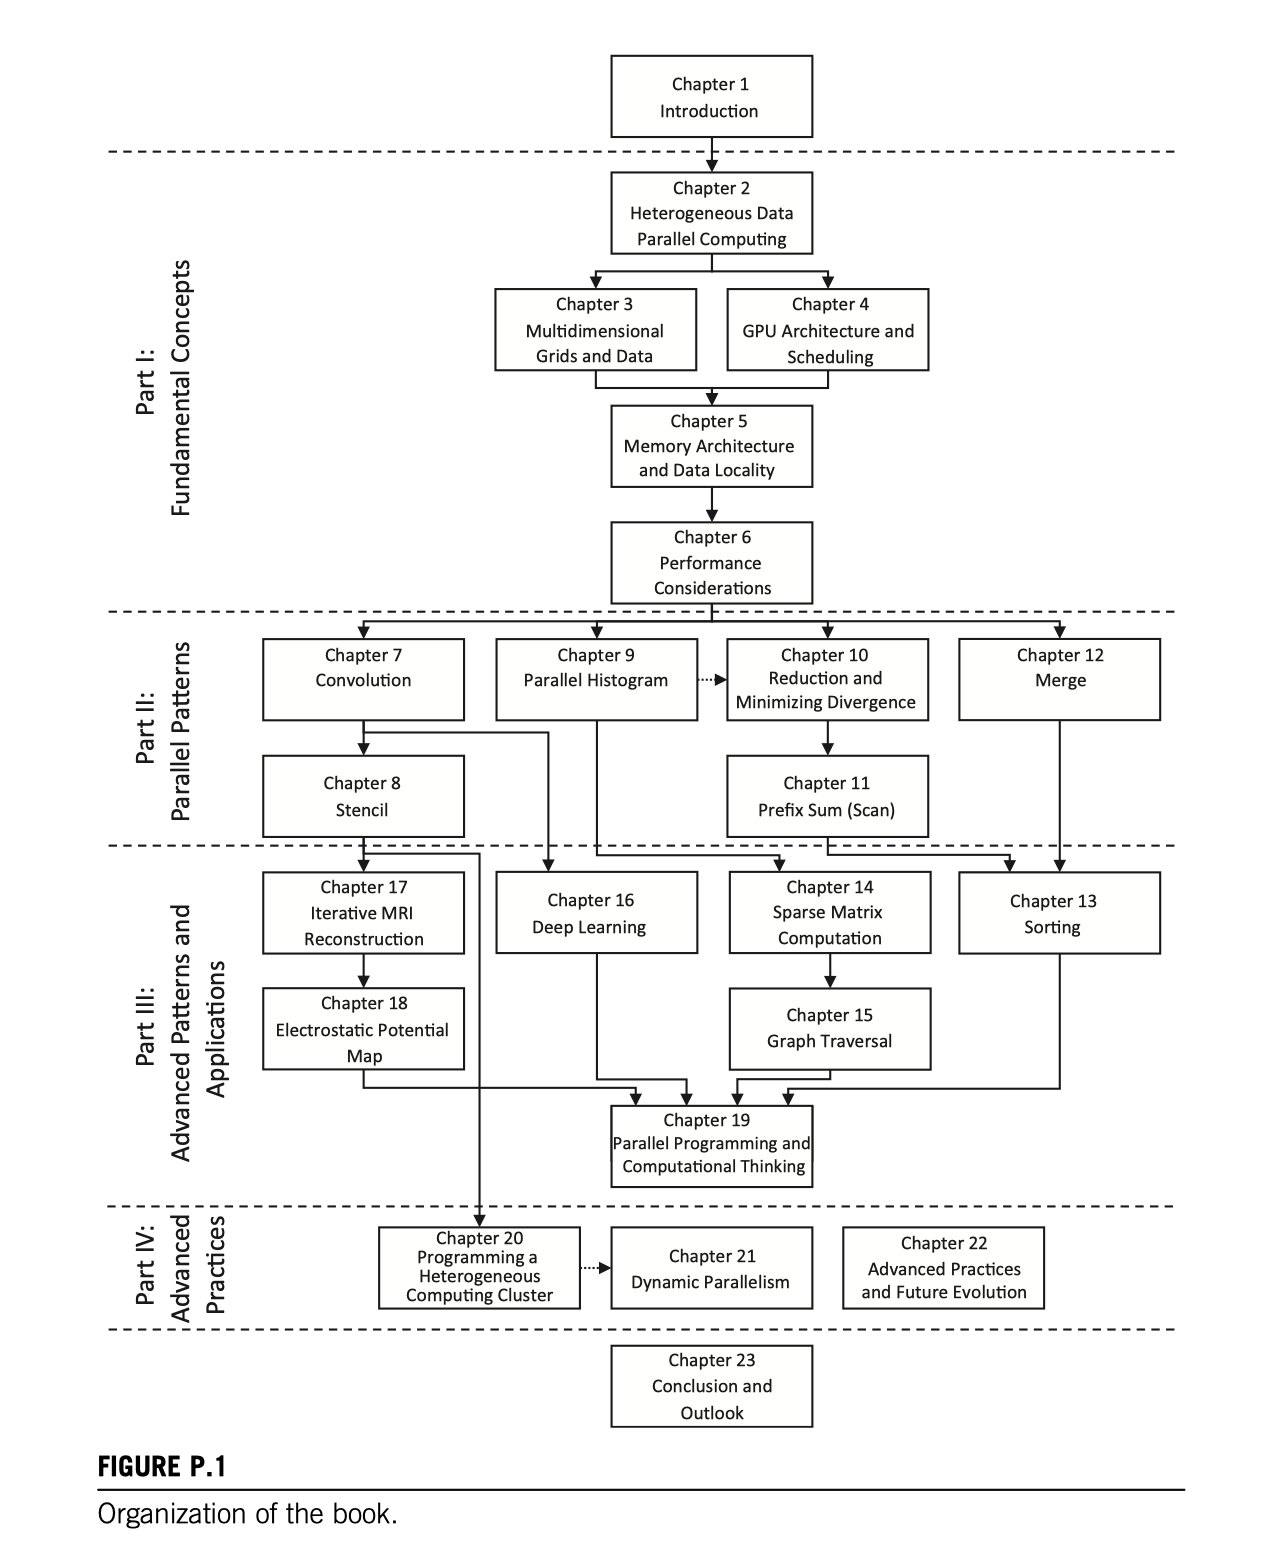
\includegraphics[width=\textwidth]{figs/P.1.png}
\end{figure}

\subsection{如何使用这本书}
我们希望通过本书提供一些教学课程的经验。 自 2006 年以来,我们教授多种类型的课程:一学期课程和一周强化课程。 
最初的 ECE498AL 课程已成为伊利诺伊大学香槟分校的永久课程,称为 ECE408 或 CS483。 
当我们第二次提供 ECE498AL 时,我们开始编写本书的一些早期章节。 
前四章也在 Nicolas Pinto 于 2009 年春天教授的麻省理工学院课程中进行了测试。
从那时起,我们将这本书用于 ECE408 的众多课程以及 Coursera 异构并行编程课程以及 VSCSE 和 PUMPS 暑期学校 。

\subsection{两阶段方法}
书中的大部分章节都设计为每节大约 75 分钟的讲座。 可能需要两节 75 分钟的讲座才能完全讲完的章节
是第 11 章(前缀和(扫描))、第 14 章(稀疏矩阵计算)和第 15 章(图遍历)。 
在 ECE408 中,讲座、编程作业和期末项目是同步进行的,并分为两个阶段。

在第一阶段,即本书的第一部分和第二部分,学生学习基础知识和基本模式,并练习通过指导性编程作业所学到的技能。 
此阶段由 12 章组成,通常需要大约 7 周的时间。 每周,学生都会完成与该周讲座相对应的编程作业。 
例如,第一周,基于第2章的讲座专门讲授基本的CUDA内存/线程模型、CUDA对C语言的扩展以及基本的编程工具。 
讲座结束后,学生可以在几个小时内编写简单的向量加法代码。

接下来的两周包括基于第 3 章到第 6 章的一系列四堂讲座,让学生对 CUDA 内存模型、CUDA 线程执行模型、
GPU 硬件性能特征和现代计算机系统架构有概念性的理解。 
在这两周内,学生们研究矩阵-矩阵乘法的不同实现,他们会看到在此期间其实现的性能如何显着提高。 
在剩下的四个星期中,讲座涵盖了基于第 7 章到第 12 章开发高性能并行应用程序所需的常见数据并行编程模式。
在这几周中,学生完成有关卷积、直方图、约简和前缀和的作业。 在第一阶段结束时,学生应该对并行编程非常熟悉,
并且应该准备好以更少的操作来实现更高级的代码。

在第二阶段(由第三部分和第四部分组成)中,学生在完成涉及加速高级模式或应用程序的最终项目时学习高级模式和应用程序。 
他们还学习了在完成项目时可能会发现有用的高级实践。 尽管我们通常不会在此阶段分配每周的编程作业,
但该项目通常有一个每周里程碑来帮助学生调整自己的节奏。 根据课程的持续时间和形式,教师可能无法涵盖此阶段的所有章节,
可能需要跳过一些章节。 教师还可以选择用客座讲座、论文讨论会或支持最终项目的讲座来代替一些讲座。 
因此,图 P.1 使用箭头来指示章节之间的依赖关系,以帮助教师选择可以跳过或重新排序的章节,以根据其特定上下文定制课程。

\subsection{将它们结合在一起:最终项目}
虽然本书的讲座、实验和章节有助于为学生奠定知识基础,但将学习经验整合在一起的是最终项目。 
最终项目对于整个学期的课程非常重要,因此它在课程中占据显着位置,需要近两个月的时间来重点关注。 
它包含五个创新方面:指导、研讨会、临床、最终报告和研讨会。 
虽然有关最终项目的大部分信息都可以在伊利诺伊州 NVIDIA GPU 教学套件中找到,但我们仍想提供这些方面设计背后的推理。

鼓励学生将他们的最终项目基于代表研究界当前挑战的问题。 为了推动这一过程,
教师应该招募几个计算科学研究小组来提出问题并担任导师。 导师被要求提供一份一到两页的项目规格表,
简要描述申请的重要性、导师希望与学生团队一起完成申请的目标、技术技能(特定类型的数学、物理) 和化学课程),
这是理解和使用应用程序所需的,以及学生可以利用的网络和传统资源列表,以获取技术背景、一般信息和构建块,
以及特定实现的特定 URL 或 FTP 路径 和编码示例。 
这些项目规格表还为学生提供了在其职业生涯后期定义自己的研究项目的学习经验。 
伊利诺伊州-NVIDIA GPU 教学套件中提供了几个示例。

\subsection{设计文档}
一旦学生决定了一个项目并组建了一个团队,他们就需要提交该项目的设计文件。 
这有助于他们在投入项目之前仔细考虑项目步骤。 进行此类规划的能力对于他们以后的职业成功非常重要。 
设计文件应讨论项目的背景和动机、应用程序级目标和潜在影响、最终应用程序的主要特征、
设计概述、实施计划、性能目标、验证计划和验收测试 ,以及项目进度表。

\subsection{项目报告及座谈会}
学生需要提交一份关于其团队主要发现的项目报告。 我们还建议举办全天的班级研讨会。 
在研讨会期间,学生使用与团队规模成比例的演示时段。 
在演示过程中,学生们为了全班同学的利益而突出了他们的项目报告中最好的部分。 
演讲占学生成绩的很大一部分。 每个学生必须单独回答针对该学生的问题,因此可以为同一团队中的个人分配不同的成绩。 
研讨会为学生提供了一个学习如何进行简洁演示的机会,以激励他们的同伴阅读全文。

\subsection{班级竞赛}
2016年ECE408的招生规模远远超过了最终项目进程所能容纳的水平。 结果,我们从期末项目变成了班级竞赛。 
在学期中期,我们宣布了一个竞赛挑战问题。 我们用一个讲座来解释比赛挑战问题以及用于对团队进行排名的规则。 
所有学生提交的内容都会自动评分和排名。 每个团队的最终排名取决于其并行代码的执行时间、正确性和清晰度。 
学生在学期结束时演示他们的解决方案并提交最终报告。 当班级规模导致最终项目不可行时,这种妥协保留了最终项目的一些好处。

\subsection{课程资源}
伊利诺伊州-NVIDIA GPU 教学套件是一个公开资源,其中包含讲座幻灯片和录音、实验作业、
最终项目指南以及为在课堂上使用本书的教师提供的示例项目规范。 此外,我们正在公开基于本书的伊利诺伊州本科生和研究生课程。 
虽然本书为这些课程提供了知识内容,但附加材料对于实现总体教育目标至关重要。

最后,我们鼓励您提交反馈。 如果您有任何改进本书的想法,我们希望收到您的来信。 我们想知道如何改进在线补充材料。 
当然,我们也想知道您喜欢这本书的哪些方面。 我们期待您的回音。


\newpage
\section*{致谢}
有很多人为第四版做出了特殊贡献。 我们首先要感谢各章节的合著者。 他们的名字列在他们做出特殊贡献的章节中。 
他们的专业知识对这个新版本的技术内容产生了巨大的影响。 如果没有这些人的专业知识和贡献,
我们就无法以我们希望向读者提供的洞察力来涵盖这些主题。

我们要特别感谢 CUDA 之父 Ian Buck 和 Tesla GPU 计算架构的首席架构师 John Nickolls。 
他们的团队为本课程构建了出色的基础设施。 NVIDIA 的许多工程师和研究人员也为 CUDA 的快速发展做出了贡献,
CUDA 支持高级并行模式的高效实现。 当我们制作第二版时,约翰去世了。 我们非常想念他。

自第三版以来,我们的外部审稿人花费了大量宝贵的时间为我们提供富有洞察力的反馈:
Sonia Lopez Alarcon(罗彻斯特理工学院)、Bedrich Benes(普渡大学)、Bryan Chin(加州大学圣地亚哥分校)、
Samuel Cho(维克森林大学) )、Kevin Farrell(爱尔兰都柏林布兰查兹敦理工学院)、
Lahouari Ghouti(沙特阿拉伯法赫德国王石油矿产大学)、Marisa Gil(西班牙巴塞罗那加泰罗尼亚理工大学)、
Karen L. Karavanic(波特兰) 州立大学)、Steve Lumetta(伊利诺伊大学厄巴纳-香槟分校)、
Dejan Milojici(惠普实验室)、Pinar Muyan-Ozcelik(加州州立大学萨克拉门托分校)、
Greg Peterson(田纳西大学诺克斯维尔分校)、Jose´L. Sa´nchez(卡斯蒂利亚拉曼恰大学)、
Janche Sang(克利夫兰州立大学)和 Jan Verschelde(伊利诺伊大学芝加哥分校)。 
他们的评论帮助我们显着提高了本书的内容和可读性。

Steve Merken、Kiruthika Govindaraju、Naomi Robertson 以及他们在爱思唯尔的员工为这个项目孜孜不倦地工作。

我们要特别感谢黄仁勋为开发这门课程提供了大量的财力和人力资源,为本书奠定了基础。

我们要感谢迪克·布拉胡特 (Dick Blahut),他向我们提出了启动该项目的挑战。 
Beth Katsinas 安排了 Dick Blahut 与 NVIDIA 副总裁 Dan Vivoli 的会面。 
通过那次聚会,Blahut 被介绍给 David,并挑战 David 来伊利诺伊州,与 Wen-mei. 一起创建原创的 ECE498AL 课程。

我们要特别感谢我们的同事 Kurt Akeley、Al Aho、Arvind、Dick Blahut、Randy Bryant、Bob Colwell、Bill Dally、
Ed Davidson、Mike Flynn、Michael Garland、John Hennessy、Pat Hanrahan、Nick Holonyak、Dick Karp、
Kurt Keutzer、Chris Lamb、Dave Liu、David Luebke、Dave Kuck、Nacho Navarro、Sanjay Patel、Yale Patt、
David Patterson、Bob Rao、Burton Smith、Jim Smith 和 Mateo Valero 花时间与我们分享了他们的见解 这些年来。

所有为这门课程和本书做出贡献的伟大人士的慷慨和热情让我们深感谦卑。


\newpage
\section{介绍}

自从计算出现以来,许多高价值应用程序都需要比计算设备所能提供的更高的执行速度和资源。 
早期应用依靠处理器速度、内存速度和内存容量的进步来增强应用级能力,如天气预报的及时性、工程结构分析的准确性、
计算机生成图形的真实性、航班预订数量等 每秒处理的资金转账数量。 
最近,深度学习等新应用程序需要比最好的计算设备所能提供的更多的执行速度和资源。 
这些应用需求在过去五年中推动了计算设备功能的快速进步,并且在可预见的未来将继续如此。

基于单个中央处理单元 (CPU) 的微处理器似乎按顺序步骤执行指令,例如 Intel 和 AMD 的 x86 处理器中的微处理器,
配备快速增加的时钟频率和硬件资源,推动了20世纪80年代和90年代的计算机应用性能的快速提高和成本的降低。 
在二十年的发展过程中,这些单 CPU 微处理器为桌面带来了 GFLOPS,即每秒千兆 ($10^9$) 次浮点运算,为数据中心带来了 TFLOPS,
即每秒万亿 ($10^{12}$) 次浮点运算。 这种对性能改进的不懈追求使得应用软件能够提供更多功能、
拥有更好的用户界面并生成更有用的结果。 反过来,一旦用户习惯了这些改进,他们就会要求更多的改进,
从而为计算机行业创造一个积极(良性)的循环。

然而,自 2003 年以来,由于能源消耗和散热问题,这种正向驱动的速度已经放缓。 
这些问题限制了时钟频率的增加以及单个 CPU 内每个时钟周期内可以执行的生产活动,同时保持了按顺序步骤执行指令的外观。 
从那时起,几乎所有微处理器供应商都转向了在每个芯片中使用多个物理 CPU(称为处理器内核)的模型,以提高处理能力。 
在这个模型中,传统的CPU可以被视为单核CPU。 为了受益于多个处理器内核,用户必须拥有多个指令序列,
无论是来自相同应用程序还是不同应用程序,都可以在这些处理器内核上同时执行。 对于要从多个处理器核心中受益的特定应用程序,
其工作必须分为可以在这些处理器核心上同时执行的多个指令序列。 
从单 CPU 按顺序执行指令到多核并行执行多个指令序列的转变对软件开发人员社区产生了巨大影响。

传统上,绝大多数软件应用程序都是作为顺序程序编写的,由处理器执行,
这些处理器的设计是冯·诺依曼在 1945 年的开创性报告中设想的(冯·诺依曼等人,1972 年)。 
人们可以将这些程序的执行理解为基于程序计数器(在文献中也称为指令指针)的概念按顺序单步执行代码。 
程序计数器包含处理器将执行的下一条指令的内存地址。 由应用程序的这种顺序、
逐步执行产生的指令执行活动序列在文献中被称为执行线程,或简称为线程。 线程的概念非常重要,
因此本书的其余部分将对其进行更正式的定义和广泛的使用。

从历史上看,大多数软件开发人员依赖硬件的进步,例如提高时钟速度和在后台执行多条指令,来提高顺序应用程序的速度; 
随着每一代新处理器的推出,相同的软件运行得更快。 计算机用户也越来越期望这些程序在每一代新一代微处理器上运行得更快。 
这种期望十多年来一直不成立。 顺序程序将仅在一个处理器内核上运行,一代又一代不会变得明显更快。 
如果没有性能改进,随着新微处理器的推出,应用程序开发人员将无法再在其软件中引入新的特性和功能; 
这减少了整个计算机行业的增长机会。

相反,每一代新一代微处理器将继续享受显着性能改进的应用软件将是并行程序,其中多个执行线程协作以更快地完成工作。 
并行程序相对于顺序程序的这种新的、显着提升的优势被称为并发革命(Sutter 和 Larus,2005)。 
并行编程的实践绝不是新鲜事。 几十年来,高性能计算 (HPC) 社区一直在开发并行程序。 
这些并行程序通常在昂贵的大型计算机上运行。 只有少数精英应用程序可以证明使用这些计算机是合理的,
从而将并行编程的实践限制在少数应用程序开发人员中。 现在所有新的微处理器都是并行计算机,
需要开发为并行程序的应用程序数量急剧增加。 现在软件开发人员非常需要学习并行编程,这也是本书的重点。

\subsection{异构并行计算}
自 2003 年以来,半导体行业已经确定了微处理器设计的两条主要轨迹(Hwu 等人,2008 年)。 
多核轨迹旨在在进入多核的同时保持顺序程序的执行速度。 多核始于两核处理器,并且核心数量随着每一代半导体工艺的发展而增加。 
最近的一个例子是最新的 Intel 多核服务器微处理器,具有多达 24 个处理器核心,每个处理器核心都是无序、多指令发布处理器,
实现完整的 x86 指令集,支持具有两个硬件线程的超线程,旨在最大限度地提高性能。 顺序程序的执行速度。 
另一个例子是最新的 ARM Ampere 多核服务器处理器,具有 128 个处理器内核。

相比之下,多线程轨迹更关注并行应用程序的执行吞吐量。 多线程轨迹始于大量线程,并且线程数量再次随着每一代的增加而增加。 
最近的一个例子是 NVIDIA Tesla A100 图形处理单元 (GPU),它具有数万个线程,在大量简单、有序的管道中执行。 
自 2003 年以来,多线程处理器,尤其是 GPU,一直在浮点性能竞赛中处于领先地位。
截至 2021 年,A100 GPU 的峰值浮点吞吐量为 64 位双精度 9.7 TFLOPS,32 位单精度 156 TFLOPS,
16 位半精度为 312 TFLOPS。 相比之下,最新的英特尔 24 核处理器的双精度峰值浮点吞吐量为 0.33 TLOPS,
单精度为 0.66 TFLOPS。 过去几年,多线程 GPU 和多核 CPU 之间的峰值浮点计算吞吐量之比一直在增加。 
这些不一定是应用程序速度; 它们只是这些芯片中执行资源可以支持的原始速度。

多核和多线程之间的峰值性能之间如此巨大的差距已经形成了显着的“电势”积累,在某些时候,必须做出一些让步。 
我们已经达到了这一点。 迄今为止,这种巨大的峰值性能差距已经促使许多应用程序开发人员将其软件的计算密集型部分转移到 
GPU 上执行。 也许更重要的是,并行执行性能的大幅提升使得革命性的新应用成为可能,例如本质上由计算密集型部分组成的深度学习。 
毫不奇怪,这些计算密集型部分也是并行编程的主要目标:当有更多工作要做时,
就有更多机会在协作的并行工作线程(即线程)之间分配工作。

{\color{red} Fig 1.1}

有人可能会问,为什么多线程 GPU 和多核 CPU 之间的峰值性能差距如此之大。 答案在于两种类型处理器之间基本设计理念的差异,
如图 1.1 所示。 如图 1.1A 所示,CPU 的设计针对顺序代码性能进行了优化。 
算术单元和操作数数据传送逻辑的设计旨在最大限度地减少算术运算的有效延迟,但代价是增加芯片面积和每单元功耗的使用。 
大型末级片上高速缓存旨在捕获频繁访问的数据,并将一些长延迟内存访问转换为短延迟高速缓存访问。 
复杂的分支预测逻辑和执行控制逻辑用于减轻条件分支指令的延迟。 通过减少操作的延迟,CPU 硬件减少了每个单独线程的执行延迟。 
然而,低延迟算术单元、复杂的操作数传送逻辑、大型高速缓冲存储器和控制逻辑消耗了芯片面积和功率,
否则这些芯片面积和功率可用于提供更多算术执行单元和存储器访问通道。 这种设计方法通常称为面向延迟的设计。

另一方面,GPU 的设计理念是由快速发展的视频游戏行业塑造的,
该行业对在高级游戏中执行大量浮点计算和每帧内存访问的能力提出了巨大的经济压力。 
这种需求促使 GPU 供应商寻找方法来最大化专用于浮点计算和内存访问吞吐量的芯片面积和功率预算。

在图形应用程序中,每秒执行大量浮点计算以完成视点变换和对象渲染等任务是非常直观的。 
此外,每秒执行大量内存访问的需求同样重要,甚至可能更重要。 
许多图形应用程序的速度受到数据从内存系统传送到处理器的速率的限制,反之亦然。 
GPU 必须能够将大量数据移入和移出其 DRAM(动态随机存取存储器)中的图形帧缓冲区,
因为这种移动可以使视频显示丰富并满足游戏玩家的需求。 
游戏应用程序普遍接受的宽松内存模型(各种系统软件、应用程序和 I/O 设备期望其内存访问工作的方式)
也使 GPU 更容易支持访问内存的大规模并行性。

相比之下,通用处理器必须满足传统操作系统、应用程序和 I/O 设备的要求,这些要求对支持并行内存访问提出了更多挑战,
从而使提高内存访问(通常称为内存)的吞吐量,常被称为内存带宽,变得更加困难。 
因此,图形芯片的运行内存带宽大约是同时可用 CPU 芯片的 10 倍,我们预计 GPU 在内存带宽方面将在一段时间内继续保持优势。

一个重要的观察是,就功耗和芯片面积而言,减少延迟比增加吞吐量要昂贵得多。 
例如,可以通过将运算单元的数量加倍来使运算吞吐量加倍,但代价是芯片面积和功耗加倍。 
然而,将算术延迟减少一半可能需要将电流加倍,但代价是所用芯片面积增加一倍以上,功耗增加四倍。 
因此,GPU 的主流解决方案是优化大量线程的执行吞吐量,而不是减少单个线程的延迟。 
这种设计方法允许流水线内存通道和算术运算具有较长的延迟,从而节省了芯片面积和功耗。 
内存访问硬件和算术单元的面积和功率的减少使得 GPU 设计者可以在芯片上拥有更多的硬件和算术单元,从而提高总执行吞吐量。 
图 1.1 通过在图 1.1A 的 CPU 设计中显示较少数量的较大算术单元和较少数量的内存通道,直观地说明了设计方法的差异,
与图 1.1B 中大量的较小算术单元和大量的存储器通道形成对比。

这些 GPU 的应用软件预计将使用大量并行线程编写。 当其中一些线程等待长延迟内存访问或算术运算时,
硬件会利用大量线程来寻找要做的工作。 图 1.1B 中的小型高速缓冲存储器用于帮助控制这些应用程序的带宽需求,
以便访问相同内存数据的多个线程不需要全部访问 DRAM。 这种设计风格通常称为面向吞吐量的设计,
因为它力求最大化大量线程的总执行吞吐量,同时允许单个线程可能需要更长的执行时间。

应该清楚的是,GPU 被设计为并行的、面向吞吐量的计算引擎,它们在某些 CPU 设计为能很好执行的任务上表现不佳。 
对于只有一个或很少线程的程序,具有较低操作延迟的CPU可以获得比GPU高得多的性能。 
当程序有大量线程时,具有较高执行吞吐量的GPU可以获得比CPU高得多的性能。 
因此,我们应该预料到许多应用程序会同时使用 CPU 和 GPU,在 CPU 上执行顺序部分,在 GPU 上执行数值密集型部分。 
这就是 NVIDIA 于 2007 年推出的统一计算设备架构 (CUDA) 编程模型旨在支持应用程序的 CPU-GPU 联合执行的原因。

还需要注意的是,当应用程序开发人员选择运行其应用程序的处理器时,速度并不是唯一的决定因素。 其他几个因素可能更为重要。 
首先也是最重要的是,所选处理器必须在市场上占有很大的份额,称为处理器的安装基础。 原因很简单。 
大量的客户群最能证明软件开发成本的合理性。 在市场份额较小的处理器上运行的应用程序不会有大量的客户群。 
这一直是传统并行计算系统的一个主要问题,与通用微处理器相比,传统并行计算系统的市场份额可以忽略不计。 
只有少数由政府和大公司资助的精英应用程序在这些传统的并行计算系统上成功开发。 多线程 GPU 改变了这种情况。 
由于 GPU 在 PC 市场的受欢迎,其销量已达数亿。 几乎所有台式电脑和高端笔记本电脑都配备了 GPU。 
迄今为止,已使用超过 10 亿个支持 CUDA 的 GPU。 如此庞大的市场占有率使这些 GPU 对应用程序开发人员来说具有经济吸引力。

另一个重要的决定因素是实用的外形因素和易于访问性。 直到 2006 年,并行软件应用程序都在数据中心服务器或部门集群上运行。 
但这样的执行环境往往会限制这些应用程序的使用。 比如在医学影像这样的应用中,发表一篇基于64节点集群机的论文就可以了。 
但磁共振成像 (MRI) 机器的实际临床应用是基于 PC 和特殊硬件加速器的某种组合。 
原因很简单,GE 和西门子等制造商无法在临床环境中销售需要计算机服务器机架的 MRI,而这在学术部门环境中很常见。 
事实上,美国国立卫生研究院 (NIH) 在一段时间内拒绝资助并行编程项目; 他们认为并行软件的影响将是有限的,
因为基于集群的大型机器无法在临床环境中工作。 如今,许多公司都配备了 GPU 的 MRI 产品,
美国国立卫生研究院 (NIH) 也资助使用 GPU 计算的研究。

直到 2006 年,图形芯片都非常难以使用,因为程序员必须使用相当于图形 API(应用程序编程接口)功能来访问处理单元,
这意味着需要 OpenGL 或 Direct3D 技术来对这些芯片进行编程。 更简单地说,计算必须表示为以某种方式绘制像素的函数,
以便在这些早期的 GPU 上执行。 该技术称为 GPGPU,用于使用 GPU 进行通用编程。 即使使用更高级别的编程环境,
底层代码仍然需要适合用于绘制像素的 API。 这些 API 限制了人们实际上可以为早期 GPU 编写的应用程序类型。 
因此,GPGPU 并没有成为一种广泛的编程现象。 尽管如此,这项技术还是足够令人兴奋,激发了一些英勇的努力和出色的研究成果。

2007 年,随着 CUDA 的发布,一切都发生了变化(NVIDIA,2007)。 CUDA 并不单独代表软件变更; 
芯片中添加了额外的硬件。 NVIDIA实际上专门投入了硅片面积以方便并行编程。 在 G80 及其后续并行计算芯片中,
GPGPU 程序根本不再通过图形接口。 相反,硅芯片上的新通用并行编程接口可以满足 CUDA 程序的要求。 
通用编程接口极大地扩展了可以轻松为 GPU 开发的应用程序类型。 所有其他软件层也都重新设计,
以便程序员可以使用熟悉的 C/C++ 编程工具。

虽然 GPU 是异构并行计算中的一类重要计算设备,但还有其他重要类型的计算设备在异构计算系统中用作加速器。 
例如,现场可编程门阵列已被广泛用于加速网络应用。 本书中介绍的使用 GPU 作为学习工具的技术也适用于这些加速器的编程任务。

\subsection{为什么要提高速度或并行性?}
正如我们在 1.1 节中所述,大规模并行编程的主要动机是让应用程序在未来的硬件世代中享受持续的速度提升。 
正如我们将在并行模式、高级模式和应用程序(第二部分和第三部分,第 7 章到第 19 章)中讨论的那样,
当应用程序适合并行执行时,在 GPU 上良好的实现可以比在单个 CPU 内核上顺序执行获得 100 倍以上的加速。
如果应用程序包含我们所说的“数据并行性”,通常只需几个小时的工作即可实现 10x 的加速。

人们可能会问为什么应用程序将继续要求提高速度。 我们今天拥有的许多应用程序似乎运行得足够快。 
尽管当今世界有无数的计算应用程序,但未来许多令人兴奋的大众市场应用程序都是我们之前认为的超级计算应用程序或超级应用程序。 
例如,生物学研究界正在越来越多地进入分子水平。 显微镜可以说是分子生物学中最重要的仪器,过去依赖光学或电子仪器。 
然而,我们使用这些仪器进行的分子水平观察存在局限性。 通过结合计算模型来模拟具有传统仪器设置的边界条件的基础分子活动,
可以有效地解决这些限制。 通过模拟,我们可以测量更多的细节并测试更多的假设,这比仅使用传统仪器所能想象的要多。 
在可预见的未来,就可建模的生物系统的规模以及可在可容忍响应时间内模拟的反应时间长度而言,这些模拟将继续受益于计算速度的提高。 
这些增强将对科学和医学产生巨大影响。

对于视频和音频编码和操作等应用,请考虑与旧式 NTSC 电视相比,我们对数字高清 (HD) 电视的满意度。 
一旦我们在高清电视上体验到图像的细节水平,就很难再回到旧技术了。 但请考虑高清电视所需的所有处理。 
这是一个高度并行的过程,三维 (3D) 成像和可视化也是如此。 
未来,视图合成和低分辨率视频的高分辨率显示等新功能将需要电视具有更高的计算能力。 
在消费者层面,我们将开始看到越来越多的视频和图像处理应用程序,这些应用程序可以改善图片和视频的焦点、光照和其他关键方面。

更高的计算速度带来的好处之一是更好的用户界面。 智能手机用户现在可以享受到与大屏幕电视相媲美的高分辨率触摸屏的更自然的界面。 
毫无疑问,这些设备的未来版本将整合具有 3D 视角的传感器和显示器、
结合虚拟和物理空间信息以增强可用性的应用程序以及基于语音和计算机视觉的界面,从而需要更高的计算速度。

消费电子游戏领域也正在进行类似的发展。 过去,在游戏中驾驶汽车只是一组预先安排好的场景。 
如果你的车撞到了障碍物,你的车的路线不会改变; 只是游戏比分发生了变化。 您的车轮没有弯曲或损坏,即使您失去了一个车轮,
驾驶也不再困难。 随着计算速度的提高,游戏可以基于动态模拟而不是预先安排的场景。 
我们可以期待在未来体验到更多这样的现实效果。 事故会损坏你的车轮,你的在线驾驶体验将会更加真实。 
精确建模物理现象的能力已经激发了数字孪生的概念,其中物理对象在模拟空间中具有精确的模型,
从而可以以更低的成本彻底进行压力测试和恶化预测。 众所周知,物理效应的真实建模和模拟需要非常大量的计算能力。

通过大幅提高计算吞吐量而实现的新应用程序的一个重要例子是基于人工神经网络的深度学习。 
虽然神经网络自 20 世纪 70 年代以来一直在积极研究,但它们在实际应用中一直无效,
因为训练这些网络需要太多的标记数据和太多的计算。 互联网的兴起提供了大量带标签的图片,GPU 的兴起带来了计算吞吐量的激增。 
因此,自 2012 年以来,基于神经网络的应用在计算机视觉和自然语言处理领域得到了快速采用。
这种采用彻底改变了计算机视觉和自然语言处理应用,并引发了自动驾驶汽车和家庭辅助设备的快速发展。

我们提到的所有新应用程序都涉及以不同方式和在不同级别模拟和/或表示物理并发世界,并处理大量数据。 
有了如此大量的数据,大部分计算可以在数据的不同部分上并行完成,尽管它们必须在某些时候进行协调。 
在大多数情况下,数据交付的有效管理会对并行应用程序的可实现速度产生重大影响。 
虽然这样做的技术通常为一些每天使用此类应用程序的专家所熟知,
但绝大多数应用程序开发人员可以从对这些技术的更直观的理解和实际工作知识中受益。

我们的目标是以直观的方式向应用程序开发人员展示数据管理技术,这些开发人员的正规教育可能不是计算机科学或计算机工程。 
我们还旨在提供许多实用的代码示例和实践练习,帮助读者获取工作知识,
这需要一个实用的编程模型来促进并行实现并支持数据交付的正确管理。 CUDA 提供了这样的编程模型,
并且已经过大型开发者社区的充分测试。

\subsection{加速实际的应用}
通过并行化应用程序,我们可以期望获得多少加速? 计算系统 A 相对于计算系统 B 的应用程序加速比的定义是,
在系统 B 中执行应用程序所用的时间与在系统 A 中执行相同应用程序所用的时间之比。
例如,如果应用程序在系统 A 中执行需要花费 10 秒,而在系统 B 中执行需要 200 秒,
则系统 A 相对于系统 B 的执行加速为 200/10=20,称为 20x(20 倍)加速。

并行计算系统相对于串行计算系统可实现的加速取决于可以并行化的应用程序部分。 
例如,如果可并行部分所花费的时间百分比为 30\%,则并行部分加速 100x 将使应用程序的总执行时间减少不超过 29.7\%。 
也就是说,整个应用程序的加速大约仅为 1/(1 - 0.297)=1.42x。 事实上,即使在并行部分进行无限量的加速,
也只能将执行时间减少 30\%,实现的加速不超过 1.433。 
通过并行执行可以实现的加速水平可能会受到应用程序的可并行部分的严重限制,这一事实被称为阿姆达尔定律(Amdahl,2013)。 
另一方面,如果 99\% 的执行时间都在并行部分,则并行部分加速 100x 会将应用程序执行时间减少到原始时间的 1.99\%。 
这使整个应用程序加速了 50x。 因此,对于大规模并行处理器来说,应用程序的绝大多数执行都在并行部分进行,
以有效加快其执行速度,这一点非常重要。

研究人员已在某些应用程序中实现了超过 100x 的加速。 然而,这通常只有在算法得到增强后进行大量优化和调整才能实现,
这样超过 99.9\% 的应用程序工作都在并行部分。

应用程序可实现的加速水平的另一个重要因素是从内存访问和写入数据的速度。 在实践中,
应用程序的直接并行化通常会导致内存 (DRAM) 带宽饱和,从而仅带来大约 10x 的加速。 诀窍在于找出如何解决内存带宽限制,
这涉及到进行多种转换之一,以利用专门的 GPU 片上内存来大幅减少对 DRAM 的访问次数。 
然而,必须进一步优化代码以克服片上内存容量有限等限制。 本书的一个重要目标是帮助读者充分理解这些优化并熟练使用它们。

请记住,单核 CPU 执行所实现的加速水平也可以反映 CPU 对应用程序的适用性。 在某些应用程序中,CPU 的性能非常好,
这使得使用 GPU 加速性能变得更加困难。 大多数应用程序都有一些可以由 CPU 更好地执行的部分。 
我们必须给CPU一个公平的执行机会,并确保编写的代码能够让GPU补充CPU的执行,
从而正确地利用CPU/GPU组合系统的异构并行计算能力。 
截至目前,结合了多核 CPU 和众核 GPU 的大众市场计算系统已经为笔记本电脑带来了万亿级计算,为集群带来了百亿亿级计算。

{\color{red} Fig 1.2}

图 1.2 说明了典型应用的主要部分。 实际应用程序的大部分代码往往是连续的。 这些连续的部分被图示为桃子的“核”区域; 
尝试将并行计算技术应用于这些部分就像咬桃核一样——感觉不太好! 这些部分很难并行化。 CPU 在这些部分往往做得非常好。 
好消息是,虽然这些部分可能占用大部分代码,但它们往往只占超级应用程序执行时间的一小部分。

然后是我们所说的“桃肉”部分。 这些部分很容易并行化,一些早期的图形应用程序也是如此。 
异构计算系统中的并行编程可以极大地提高这些应用程序的速度。 如图1.2所示,早期的GPGPU编程接口只覆盖了桃肉部分的一小部分,
这类似于最令人兴奋的应用程序的一小部分。 正如我们将看到的,CUDA 编程接口旨在涵盖令人兴奋的应用程序的更大部分。 
并行编程模型及其底层硬件仍在快速发展,以实现更大的应用程序部分的高效并行化。

\subsection{并行编程中的挑战}
是什么让并行编程变得困难? 有人曾经说过,如果不关心性能,并行编程是很容易的。 您实际上可以在一小时内编写一个并行程序。 
但是,如果您不关心性能,为什么还要编写并行程序呢?

本书解决了在并行编程中实现高性能的几个挑战。 首先,设计具有与顺序算法相同的算法(计算)复杂度的并行算法可能具有挑战性。 
许多并行算法执行与顺序算法相同的工作量。 然而,一些并行算法比顺序算法做更多的工作。 事实上,有时他们可能会做太多的工作,
以至于最终在大型输入数据集上运行速度变慢。 这尤其是一个问题,因为快速处理大型输入数据集是并行编程的重要动机。

例如,许多现实世界的问题最自然地用数学递归来描述。 并行化这些问题通常需要以非直观的方式思考问题,
并且可能需要在执行过程中进行冗余工作。 有一些重要的算法原语,例如前缀和,可以促进将问题的顺序递归公式转换为更并行的形式。 
我们将更正式地介绍工作效率的概念,并将说明设计并行算法所涉及的方法和权衡,
这些算法可以使用重要的并行模式(例如第 11 章“前缀”中的前缀和)实现与顺序算法相同水平的计算复杂性 总和(扫描)。

其次,许多应用程序的执行速度受到内存访问延迟和/或吞吐量的限制。 我们将这些应用程序称为内存限制应用程序; 
相比之下,计算密集型应用程序受到每字节数据执行的指令数量的限制。 
在内存受限的应用程序中实现高性能并行执行通常需要提高内存访问速度的方法。 
我们将在第 5 章“内存架构和数据局部性”和第 6 章“性能注意事项”中介绍内存访问的优化技术,
并将在有关并行模式和应用程序的几个章节中应用这些技术。

第三,并行程序的执行速度通常比顺序程序的情况对输入数据特征更敏感。 许多现实世界的应用程序需要处理具有广泛变化特征的输入,
例如不稳定或不可预测的数据大小以及不均匀的数据分布。 这些大小和分布的变化可能会导致分配给并行线程的工作量不均匀,
并可能显着降低并行执行的效率。 并行程序的性能有时会因这些特征而发生巨大变化。 
我们将在介绍并行模式和应用程序的章节中介绍用于规范数据分布和/或动态细化线程数量的技术,以应对这些挑战。

第四,某些应用程序可以并行化,同时几乎不需要跨不同线程进行协作。 这些应用程序通常被称为“令人尴尬的并行”。 
其他应用程序需要线程相互协作,这需要使用同步操作,例如屏障或原子操作。 这些同步操作给应用程序带来了开销,
因为线程经常会发现自己在等待其他线程而不是执行有用的工作。 我们将在本书中讨论减少同步开销的各种策略。

幸运的是,研究人员已经解决了大部分挑战。 跨应用程序域还存在一些常见模式,
使我们能够将在一个域中派生的解决方案应用于其他域中的挑战。 
这是我们将在重要的并行计算模式和应用程序的背景下提出解决这些挑战的关键技术的主要原因。

\subsection{相关并行编程接口}
在过去的几十年里,人们提出了许多并行编程语言和模型(Mattson 等,2004)。 
最广泛使用的是用于共享内存多处理器系统的 OpenMP(Open,2005)和用于可扩展集群计算的消息传递接口(MPI)(MPI,2009)。 
两者都已成为主要计算机供应商支持的标准化编程接口。

OpenMP 实现由编译器和运行时组成。 程序员向 OpenMP 编译器指定有关循环的指令(命令)和编译指示(提示)。 
通过这些指令和编译指示,OpenMP 编译器可以生成并行代码。 运行时系统通过管理并行线程和资源来支持并行代码的执行。 
OpenMP 最初是为 CPU 执行而设计的,现已扩展为支持 GPU 执行。 OpenMP 的主要优点是它提供编译器自动化和运行时支持,
以从程序员那里抽象出许多并行编程细节。 
这种自动化和抽象有助于使应用程序代码在不同供应商生产的系统以及同一供应商的不同代系统之间更加可移植。 
我们将此属性称为性能可移植性。 然而,在 OpenMP 中进行有效的编程仍然需要程序员了解所涉及的所有详细的并行编程概念。 
由于 CUDA 为程序员提供了对这些并行编程细节的明确控制,因此即使对于那些想要使用 OpenMP 作为主要编程接口的人来说,
它也是一种极好的学习工具。 此外,根据我们的经验,OpenMP 编译器仍在不断发展和改进。 
许多程序员可能需要使用 CUDA 风格的接口来处理 OpenMP 编译器无法满足的部分。

另一方面,MPI 是一种编程接口,其中集群中的计算节点不共享内存(MPI,2009)。 
所有的数据共享和交互都必须通过显式的消息传递来完成。 MPI在HPC中得到了广泛的应用。 
用MPI编写的应用程序已在超过10万个节点的集群计算系统上成功运行。 如今,许多 HPC 集群都采用异构 CPU/GPU 节点。 
由于计算节点之间缺乏共享内存,将应用程序移植到 MPI 所需的工作量可能相当大。 
程序员需要执行域分解以跨各个节点划分输入和输出数据。 在域分解的基础上,
程序员还需要调用消息发送和接收函数来管理节点之间的数据交换。 相比之下,
CUDA 为 GPU 中的并行执行提供共享内存来解决这一难题。 虽然 CUDA 是与每个节点的有效接口,
但大多数应用程序开发人员需要使用 MPI 在集群级别进行编程。 
此外,通过 NVIDIA Collective Communications Library (NCCL) 等 API,CUDA 中的多 GPU 编程支持不断增加。 
因此,HPC 中的并行程序员了解如何在使用多 GPU 节点的现代计算集群中进行联合 MPI/CUDA 编程非常重要,
该主题将在第 20 章“异构计算集群编程”中介绍。

2009 年,包括 Apple、Intel、AMD/ATI 和 NVIDIA 在内的几家主要行业参与者联合开发了一种名为
开放计算语言 (OpenCL) 的标准化编程模型(The Khronos Group,2009)。 与 CUDA 类似,
OpenCL 编程模型定义了语言扩展和运行时 API,以允许程序员管理大规模并行处理器中的并行性和数据交付。 
与 CUDA 相比,OpenCL 更多地依赖 API,更少地依赖语言扩展。 
这使得供应商能够快速调整其现有的编译器和工具来处理 OpenCL 程序。 OpenCL 是一种标准化的编程模型,
用 OpenCL 开发的应用程序无需修改即可在所有支持 OpenCL 语言扩展和 API 的处理器上正确运行。 
然而,人们可能需要修改应用程序才能实现新处理器的高性能。

熟悉 OpenCL 和 CUDA 的人都知道,OpenCL 和 CUDA 的关键概念和功能之间存在显着的相似性。 
也就是说,CUDA程序员可以以最小的努力学习OpenCL编程。 更重要的是,
几乎所有在使用 CUDA 中学到的技术都可以轻松应用于 OpenCL 编程。

\subsection{总体目标}
我们的主要目标是教读者如何对大规模并行处理器进行编程以实现高性能。 
因此,本书的大部分内容都致力于开发高性能并行代码的技术。 我们的方法不需要大量的硬件专业知识。 
然而,您需要对并行硬件架构有一个很好的概念性理解,以便能够推断代码的性能行为。 
因此,我们将用一些篇幅来直观地理解基本的硬件架构特性,并用许多篇幅来介绍开发高性能并行程序的技术。 
特别是,我们将重点关注计算思维(Wing,2006)技术,这些技术将使您能够以适合大规模并行处理器上高性能执行的方式思考问题。

大多数处理器上的高性能并行编程需要了解硬件的工作原理。 可能需要很多年才能构建工具和机器,
使程序员能够在没有这些知识的情况下开发高性能代码。 即使我们有这样的工具,
我们怀疑了解硬件知识的程序员将能够比那些不了解硬件的程序员更有效地使用这些工具。 
因此,我们专门用第 4 章“计算架构和调度”来介绍 GPU 架构的基础知识。 
作为高性能并行编程技术讨论的一部分,我们还讨论了更专业的体系结构概念。

我们的第二个目标是教授并行编程的正确功能和可靠性,这是并行计算中的一个微妙问题。 
过去从事并行系统工作的程序员都知道,仅实现初始性能是不够的。 挑战在于以一种可以调试代码并支持用户的方式来实现它。 
CUDA 编程模型鼓励使用简单形式的屏障同步、内存一致性和原子性来管理并行性。 
此外,它还提供了一系列强大的工具,使人们不仅可以调试功能方面,还可以调试性能瓶颈。 
我们将证明,通过关注数据并行性,可以在应用程序中实现高性能和高可靠性。

我们的第三个目标是通过探索并行编程方法来实现未来硬件各代的可扩展性,
以便未来的机器(将越来越并行)可以比今天的机器更快地运行代码。 我们希望帮助您掌握并行编程,
以便您的程序可以扩展到新一代机器的性能水平。 这种可扩展性的关键是规范和本地化内存数据访问,
以最大限度地减少关键资源的消耗和更新数据结构时的冲突。 
因此,开发高性能并行代码的技术对于确保应用程序未来的可扩展性也很重要。

实现这些目标需要大量的技术知识,因此我们将在本书中介绍并行编程的相当多的原理和模式(Mattson et al., 2004)。 
我们不会单独教授这些原则和模式。 我们将在并行化有用应用程序的背景下教授他们。 
然而,我们无法涵盖所有这些技术,因此我们选择了最有用且经过充分验证的技术来详细介绍。 
事实上,当前版本有关并行模式的章节数量显着增加。 现在我们准备向您提供本书其余部分的快速概述。

\subsection{本书的组织}
本书分为四个部分。 第一部分涵盖并行编程、数据并行、GPU 和性能优化的基本概念。 
这些基础章节为读者提供了成为 GPU 程序员所需的基本知识和技能。 第二部分介绍了原始并行模式,
第三部分介绍了更高级的并行模式和应用程序。 这两部分应用了第一部分中学到的知识和技能,
并根据需要介绍了其他 GPU 架构特性和优化技术。 最后一部分(第四部分)介绍了高级实践,
以帮助想要成为专家 GPU 程序员的读者完善知识。

关于基本概念的第一部分由第 2 章至第 6 章组成。 第 2 章,异构数据并行计算,介绍数据并行性和 CUDA C 编程。 
本章依赖于读者之前具有 C 编程经验的事实。 它首先介绍了 CUDA C 作为 C 的简单、小型扩展,
支持异构 CPU/GPU 计算和广泛使用的单程序、多数据并行编程模型。 
然后,它涵盖了以下方面所涉及的思维过程:(1) 识别要并行化的应用程序部分,
(2) 隔离并行化代码要使用的数据,使用 API 函数在并行计算设备上分配内存, (3)使用API函数将数据传输到并行计算设备,
(4)将并行部分开发为将由并行线程执行的内核函数,(5)启动由并行线程执行的内核函数,
以及( 6) 最终通过 API 函数调用将数据传输回主机处理器。 我们使用向量加法的运行示例来说明这些概念。 
虽然本章的目标是教授 CUDA C 编程模型的足够概念,以便读者能够编写简单的并行 CUDA C 程序,
但它涵盖了开发基于任何并行编程接口的并行应用程序所需的几种基本技能。

第 3 章“多维网格和数据”介绍了 CUDA 并行执行模型的更多细节,特别是它涉及使用线程的多维组织处理多维数据。 
它对线程的创建、组织、资源绑定和数据绑定提供了足够的洞察力,使读者能够使用 CUDA C 实现复杂的计算。

第 4 章,计算架构和调度,介绍 GPU 架构,重点介绍如何组织计算核心以及如何调度线程在这些核心上执行。 
讨论了各种架构注意事项,以及它们对 GPU 架构上执行的代码性能的影响。 其中包括透明可扩展性、SIMD 执行和控制发散、
多线程和延迟容忍以及占用等概念,所有这些都在本章中进行了定义和讨论。

第 5 章“内存架构和数据局部性”通过讨论 GPU 的内存架构来扩展第 4 章“计算架构和调度”。 
它还讨论了可用于保存 CUDA 变量以管理数据传输和提高程序执行速度的特殊存储器。 
我们介绍分配和使用这些内存的 CUDA 语言功能。 适当地使用这些存储器可以极大地提高数据访问吞吐量,
并有助于缓解存储器系统中的流量拥塞。

第 6 章“性能注意事项”介绍了当前 CUDA 硬件中的几个重要的性能注意事项。 
特别是,它提供了有关所需的线程执行和内存访问模式的更多详细信息。 
这些细节构成了程序员推理其组织计算和数据决策的后果的概念基础。 
本章最后列出了 GPU 程序员经常用来优化任何计算模式的常见优化策略清单。 
该清单将在本书的接下来的两部分中使用,以优化各种并行模式和应用程序。

关于原始并行模式的第二部分由第 7 章至第 12 章组成。 第 7 章“卷积”介绍了卷积,这是一种常用的并行计算模式,
植根于数字信号处理和计算机视觉,需要仔细管理数据访问局部性。 我们还使用这种模式在现代 GPU 中引入恒定内存和缓存。 
第 8 章“模板”介绍了模板,这是一种类似于卷积的模式,但植根于求解微分方程,
并且具有为进一步优化数据访问局部性提供独特机会的特定功能。 我们还使用此模式来介绍线程和数据的 3D 组织,
并展示第 6 章“性能注意事项”中介绍的针对线程粒度的优化。

第 9 章“并行直方图”介绍了直方图,这是一种广泛用于统计数据分析以及大型数据集中的模式识别的模式。 
我们还使用这种模式引入原子操作作为协调共享数据并发更新和私有化优化的手段,从而减少了这些操作的开销。 
第 10 章“归约和最小化分支”介绍了归约树模式,该模式用于总结输入数据的集合。 
我们还使用此模式来演示控制分支发散对性能的影响,并展示如何减轻这种影响的技术。 
第 11 章“前缀和(扫描)”介绍了前缀和或扫描,这是一种重要的并行计算模式,它将固有的顺序计算转换为并行计算。 
我们还使用这种模式来引入并行算法中工作效率的概念。 最后,第 12 章“合并”介绍了并行合并,
这是一种在分而治之工作分区策略中广泛使用的模式。 我们还用本章来介绍动态输入数据的识别和组织。

关于高级并行模式和应用程序的第三部分在精神上与第二部分类似,但所涵盖的模式更详细,并且通常包含更多应用程序上下文。 
因此,这些章节不太关注介绍新技术或功能,而是更关注特定于应用程序的注意事项。 对于每个应用程序,
我们首先确定制定并行执行基本结构的替代方法,然后推理每个替代方案的优点和缺点。 
然后,我们完成实现高性能所需的代码转换步骤。 这些章节帮助读者将前面章节中的所有材料放在一起,
并在他们承担自己的应用程序开发项目时为他们提供支持。

第三部分由第 13 章至第 19 章组成。 第 13 章“排序”介绍了并行排序的两种形式:基数排序和合并排序。 
这种高级模式利用了前面章节中介绍的更原始的模式,特别是前缀和和并行合并。 第 14 章,稀疏矩阵计算,介绍了稀疏矩阵计算,
它广泛用于处理非常大的数据集。 本章向读者介绍了重新排列数据以实现更有效的并行访问的概念:数据压缩、填充、排序、转置
和正则化。 第 15 章,图遍历,介绍图算法以及如何在 GPU 编程中有效地实现图搜索。 提出了许多不同的并行图算法策略,
并讨论了图结构对最佳算法选择的影响。 这些策略建立在更原始的模式之上,例如直方图和合并。

第 16 章“深度学习”涵盖了深度学习,它正在成为 GPU 计算的一个极其重要的领域。 我们介绍了卷积神经网络的有效实现,
并将更深入的讨论留给其他来源。 卷积神经网络的高效实现利用了平铺等技术和卷积等模式。 第 17 章,迭代磁共振成像重建,
涵盖非笛卡尔 MRI 重建以及如何利用循环融合和分散-聚集变换等技术来增强并行性并减少同步开销。 第 18 章,静电势图,
涵盖了分子可视化和分析,这得益于通过应用稀疏矩阵计算中的经验教训来处理不规则数据的技术。

第 19 章“并行编程和计算思维”介绍了计算思维,即以更适合 HPC 的方式制定和解决计算问题的艺术。 
它通过涵盖组织程序的计算任务以使它们可以并行完成的概念来实现这一点。 我们首先讨论将抽象的科学、
特定问题的概念组织成计算任务的转化过程,这是生产高质量串行或并行应用软件的重要的第一步。 
然后本章讨论并行算法结构及其对应用程序性能的影响,这是基于 CUDA 性能调优经验。 
尽管我们没有深入探讨这些替代并行编程风格的实现细节,
但我们希望读者能够利用在本书中获得的基础来学习其中任何一种编程风格的编程。 
我们还提出了一个高级案例研究,以展示通过创造性计算思维可以看到的机会。

第四部分高级实践由第 20 至 22 章组成。 第 20 章,异构计算集群编程,介绍了异构集群上的 CUDA 编程,
其中每个计算节点都由 CPU 和 GPU 组成。 
我们讨论使用 MPI 和 CUDA 来集成节点间计算和节点内计算以及由此产生的通信问题和实践。 
第 21 章“CUDA 动态并行性”介绍了动态并行性,即 GPU 根据数据或程序结构动态为自身创建工作的能力,
而不是总是等待 CPU 这样做。 第 22 章“高级实践和未来发展”列出了 CUDA 程序员需要了解的重要的各种高级功能和实践。 
其中包括零复制内存、统一虚拟内存、多个内核同时执行、函数调用、异常处理、调试、分析、双精度支持、
可配置缓存/暂存器大小等主题。 例如,早期版本的 CUDA 在 CPU 和 GPU 之间提供有限的共享内存功能。 
程序员需要显式管理 CPU 和 GPU 之间的数据传输。 然而,当前版本的 CUDA 支持统一虚拟内存和零拷贝内存等功能,
可实现 CPU 和 GPU 之间的数据无缝共享。 有了这样的支持,CUDA 程序员可以将变量和数据结构声明为在 CPU 和 GPU 之间共享。 
运行时硬件和软件保持一致性,并根据需要自动代表程序员执行优化的数据传输操作。 
这种支持显着降低了与计算和 I/O 活动重叠的数据传输所涉及的编程复杂性。 在教科书的介绍部分,
我们使用 API 进行显式数据传输,以便读者更好地了解幕后发生的情况。 
我们稍后会在第 22 章“高级实践和未来演进”中介绍统一虚拟内存和零拷贝内存。

虽然本书中的章节都是基于 CUDA 的,但它们总体上帮助读者建立了并行编程的基础。 
我们相信,当我们从具体的例子中学习时,人类能够最好地理解。 也就是说,我们必须首先在特定编程模型的上下文中学习概念,
这为我们将知识推广到其他编程模型时提供了坚实的基础。 当我们这样做时,我们可以从 CUDA 示例中汲取具体经验。 
对CUDA的深入体验也使我们变得成熟,这将有助于我们学习甚至可能与CUDA模型无关的概念。

第 23 章“结论和展望”提供了结论性意见以及对大规模并行编程的未来的展望。 我们首先重新审视我们的目标,
并总结各章如何组合在一起以帮助实现目标。 最后,我们预测大规模并行计算的快速进步将使其成为未来十年最令人兴奋的领域之一。


\newpage
\section{异构数据并行计算}

数据并行是指对数据集的不同部分执行的计算工作可以彼此独立地完成,从而可以彼此并行地完成的现象。 许多应用程序表现出丰富的数据并行性,这使得它们适合可扩展的并行执行。 因此,并行程序员熟悉数据并行性的概念以及编写利用数据并行性的代码的并行编程语言结构非常重要。 在本章中,我们将使用 CUDA C 语言结构来开发一个简单的数据并行程序。

\subsection{数据并行}
当现代软件应用程序运行缓慢时,问题通常是数据——数据太多而无法处理。 图像处理应用程序处理具有数百万到数万亿像素的图像或视频。 科学应用程序使用数十亿个网格点对流体动力学进行建模。 分子动力学应用必须模拟数千到数十亿个原子之间的相互作用。 航空公司的调度涉及数千个航班、机组人员和机场登机口。 大多数像素、粒子、网格点、交互、飞行等通常可以在很大程度上独立处理。 例如,在图像处理中,将彩色像素转换为灰度仅需要该像素的数据。 模糊图像会平均每个像素的颜色与附近像素的颜色,仅需要该小像素邻域的数据。 即使是看似全局的操作,例如查找图像中所有像素的平均亮度,也可以分解为许多可以独立执行的较小计算。 这种对不同数据块的独立评估是数据并行性的基础。 编写数据并行代码需要(重新)组织围绕数据的计算,以便我们可以并行执行最终的独立计算,从而更快地完成整个工作——通常要快得多。

让我们通过一个彩色到灰度转换的例子来说明数据并行的概念。 图 2.1 显示了由许多像素组成的彩色图像(左侧),每个像素包含从 0(黑色)到 1(全强度)变化的红色、绿色和蓝色分数值(r、g、b)。

为了将彩色图像(图 2.1 左侧)转换为灰度图像(右侧),我们通过应用以下加权和公式计算每个像素的亮度值 L:
\begin{equation*}
	L = r*0.21 + g*0.72 + b * 0.07
\end{equation*}

\begin{remark}[RGB 彩色图像表示]
	在 RGB 表示中,图像中的每个像素都存储为 (r, g, b) 值的元组。 图像行的格式为 (r g b) (r g b) 。 。 。 (r g b),如下面的概念图所示。 每个元组指定红色 (R)、绿色 (G) 和蓝色 (B) 的混合。 也就是说,对于每个像素,r、g、b 值代表渲染该像素时红、绿、蓝光源的强度(0 为暗,1 为全强度)。

这三种颜色的实际允许混合因行业指定的颜色空间而异。 这里,AdbobeRGBt 颜色空间中三种颜色的有效组合显示为三角形的内部。 每个混合的垂直坐标(y 值)和水平坐标(x 值)显示应为 G 和 R 的像素强度分数。像素强度的剩余分数 (1-yÀx) 应分配给 B。 渲染图像时,每个像素的 r、g、b 值用于计算像素的总强度(亮度)以及混合系数(x、y、1-y-x)。
\end{remark}

如果我们将输入视为由 RGB 值数组 I 组织的图像,并将输出视为相应的亮度值数组 O,则我们得到如图 2.2 所示的简单计算结构。 例如,根据上式计算I[0]中RGB值的加权和,生成O[0]; O[1]是通过计算I[1]中RGB值的加权和生成的; O[2]是通过计算I[2]中RGB值的加权和生成的; 等等。 这些每像素计算都不相互依赖。 所有这些都可以独立执行。 显然,彩色到灰度的转换表现出丰富的数据并行性。 当然,完整应用程序中的数据并行性可能更加复杂,本书的大部分内容都致力于教授发现和利用数据并行性所必需的并行思维。

\begin{remark}[任务并行与数据并行]
数据并行并不是并行编程中使用的唯一并行类型。 任务并行性也广泛应用于并行编程中。 任务并行性通常通过应用程序的任务分解来暴露。 例如,一个简单的应用程序可能需要进行向量加法和矩阵向量乘法。 其中每一个都是一项任务。 如果两个任务可以独立完成,则存在任务并行性。 I/O 和数据传输也是常见的任务源。

在大型应用程序中,通常存在大量独立任务,因此任务并行性也较大。 例如,在分子动力学模拟器中,自然任务列表包括振动力、旋转力、非键合力的邻居识别、非键合力、速度和位置以及基于速度和位置的其他物理属性。

一般来说,数据并行性是并行程序可扩展性的主要来源。 对于大型数据集,人们通常可以找到丰富的数据并行性,以便能够利用大规模并行处理器,并允许应用程序性能随着每一代具有更多执行资源的硬件而增长。 尽管如此,任务并行性也可以在实现性能目标方面发挥重要作用。 稍后在介绍流时我们将介绍任务并行性。
\end{remark}

\subsection{CUDA C程序结构}
我们现在准备学习如何编写 CUDA C 程序来利用数据并行性来加快执行速度。 CUDA C 1 以最少的新语法和库函数扩展了流行的 ANSI C 编程语言,使程序员能够针对包含 CPU 内核和大规模并行 GPU 的异构计算系统。 顾名思义,CUDA C 构建在 NVIDIA 的 CUDA 平台上。 CUDA是目前最成熟的大规模并行计算框架。 它广泛应用于高性能计算行业,在最常见的操作系统上提供编译器、调试器和分析器等基本工具。

CUDA C 程序的结构反映了计算机中主机(CPU)和一个或多个设备(GPU)的共存。 每个 CUDA C 源文件可以混合有主机代码和设备代码。 默认情况下,任何传统 C 程序都是仅包含主机代码的 CUDA 程序。 人们可以将设备代码添加到任何源文件中。 设备代码清楚地标有特殊的 CUDA C 关键字。 设备代码包括函数或内核,其代码以数据并行方式执行。

CUDA 程序的执行如图 2.3 所示。 执行从主机代码(CPU 串行代码)开始。 当调用内核函数时,设备上会启动大量线程来执行内核。 由内核调用启动的所有线程统称为网格。 这些线程是 CUDA 平台中并行执行的主要工具。 图 2.3 显示了两个线程网格的执行情况。 我们将很快讨论这些网格是如何组织的。 当网格的所有线程都完成其执行时,网格终止,并且执行在主机上继续,直到启动另一个网格。 请注意,图 2.3 显示了一个简化模型,其中 CPU 执行和 GPU 执行不重叠。 许多异构计算应用程序管理重叠的 CPU 和 GPU 执行,以充分利用 CPU 和 GPU。

启动网格通常会生成许多线程来利用数据并行性。 在彩色到灰度转换的示例中,每个线程可用于计算输出数组 O 的一个像素。在这种情况下,网格启动应生成的线程数等于 图片。 对于大图像,会产生大量线程。 由于高效的硬件支持,CUDA 程序员可以假设这些线程只需很少的时钟周期即可生成和调度。 这一假设与传统的 CPU 线程形成对比,传统的 CPU 线程通常需要数千个时钟周期来生成和调度。 在下一章中,我们将展示如何实现颜色到灰度转换和图像模糊内核。 在本章的其余部分中,为了简单起见,我们将使用向量加法作为运行示例。

\begin{remark}[线程]
线程是现代计算机中处理器如何执行顺序程序的简化视图。 线程由程序代码、正在执行的代码中的点及其变量和数据结构的值组成。 就用户而言,线程的执行是顺序的。 人们可以使用源代码级调试器来监视线程的进度,方法是一次执行一个语句,查看下一个将要执行的语句,并在执行过程中检查变量和数据结构的值。

线程在编程中的应用已经很多年了。 如果程序员想要在应用程序中开始并行执行,他/她可以使用线程库或特殊语言创建和管理多个线程。 在 CUDA 中,每个线程的执行也是顺序的。 CUDA 程序通过调用内核函数来启动并行执行,这会导致底层运行时机制启动并行处理数据不同部分的线程网格。
\end{remark}

\subsection{向量加法核函数}
我们使用向量加法来演示 CUDA C 程序结构。 向量加法可以说是最简单的数据并行计算——相当于顺序编程中的“Hello World”。 在我们展示向量加法的内核代码之前,首先回顾一下传统向量加法(主机代码)函数的工作原理会很有帮助。 图 2.4 显示了一个简单的传统 C 程序,由主函数和向量加法函数组成。 在我们所有的示例中,每当需要区分主机和设备数据时,我们都会在主机使用的变量名称后添加“\_h”,在设备使用的变量名称后添加“\_d”以 提醒我们自己这些变量的预期用途。 由于图 2.4 中只有主机代码,因此我们只能看到后缀为“\_h”的变量。

假设要相加的向量存储在主程序中分配并初始化的数组A和B中。 输出向量位于数组C中,该数组也在主程序中分配。 为了简洁起见,我们没有显示 A、B 和 C 在主函数中如何分配或初始化的细节。 指向这些数组的指针连同包含向量长度的变量 N 一起传递给 vecAdd 函数。 请注意,vecAdd 函数的参数带有“\_h”后缀,以强调它们是由主机使用的。 当我们在接下来的几个步骤中引入设备代码时,这种命名约定将会很有帮助。

图 2.4 中的 vecAdd 函数使用 for 循环来迭代向量元素。 在第 i 次迭代中,输出元素 C\_h[i] 接收 A\_h[i] 和 B\_h[i] 的和。 向量长度参数 n 用于控制循环,使迭代次数与向量的长度相匹配。 该函数分别通过指针A\_h、B\_h和C\_h读取A和B的元素并写入C的元素。 当vecAdd函数返回时,main函数中的后续语句就可以访问C的新内容。

并行执行向量加法的一种直接方法是修改 vecAdd 函数并将其计算移至设备。 这种修改后的 vecAdd 函数的结构如图 2.5 所示。 该函数的第 1 部分在设备 (GPU) 内存中分配空间来保存 A、B 和 C 向量的副本,并将 A 和 B 向量从主机内存复制到设备内存。 第 2 部分调用实际的向量加法内核来启动设备上的线程网格。 第 3 部分将和向量 C 从设备内存复制到主机内存,并从设备内存中释放三个数组。

请注意,修改后的 vecAdd 函数本质上是一个外包代理,它将输入数据发送到设备,激活设备上的计算,并从设备收集结果。 代理这样做的方式是主程序甚至不需要知道矢量加法现在实际上是在设备上完成的。 在实践中,这种“透明”的外包模式可能非常低效,因为所有数据都来回复制。 人们通常会在设备上保留大型且重要的数据结构,并简单地从主机代码中调用它们上的设备功能。 不过,现在我们将使用简化的透明模型来介绍基本的 CUDA C 程序结构。 修改后的函数的细节以及内核函数的编写方式将是本章剩余部分的主题。

\subsection{设备全局内存和数据传输}
在当前的 CUDA 系统中,设备通常是硬件卡,带有自己的动态随机存取存储器,称为设备全局存储器,或简称为全局存储器。 例如,NVIDIA Volta V100 配备 16GB 或 32GB 全局内存。 将其称为“全局”内存,将其与程序员也可以访问的其他类型的设备内存区分开来。 有关 CUDA 内存模型和不同类型设备内存的详细信息将在第 5 章“内存架构和数据局部性”中讨论。

对于向量加法内核,在调用内核之前,程序员需要在设备全局内存中分配空间,并将数据从主机内存传输到设备全局内存中分配的空间。 这对应于图 2.5 的第 1 部分。 类似地,在设备执行之后,程序员需要将结果数据从设备全局存储器传输回主机存储器,并释放设备全局存储器中不再需要的已分配空间。 这对应于图 2.5 的第 3 部分。 CUDA运行时系统(通常在主机上运行)提供应用程序编程接口(API)函数来代表程序员执行这些活动。 从现在开始,我们将简单地说数据从主机传输到设备,作为数据从主机内存复制到设备全局内存的简写。 对于相反的方向也是如此。

图2.5中,vecAdd函数的第1部分和第3部分需要使用CUDA API函数为A、B和C分配设备全局内存; 将 A 和 B 从主机传输到设备; 向量相加后将 C 从设备传输到主机; 并释放A、B、C的设备全局内存。我们首先解释内存分配和释放函数。

图 2.6 显示了两个用于分配和释放设备全局内存的 API 函数。 可以从主机代码调用 cudaMalloc 函数来为对象分配一块设备全局内存。 读者应该注意到 cudaMalloc 和标准 C 运行时库 malloc 函数之间惊人的相似性。 这是故意的; CUDA C 是具有最少扩展的 C。 CUDA C使用标准C运行时库malloc函数来管理主机内存2,并将cudaMalloc作为C运行时库的扩展添加。 通过使接口尽可能接近原始 C 运行时库,CUDA C 最大限度地减少了 C 程序员重新学习这些扩展的使用所花费的时间。

cudaMalloc 函数的第一个参数是指针变量的地址,该变量将被设置为指向分配的对象。 指针变量的地址应转换为 (void à ),因为该函数需要一个通用指针; 内存分配函数是一个通用函数,不限于任何特定类型的对象。 3 该参数允许 cudaMalloc 函数将分配的内存的地址写入提供的指针变量,无论其类型如何。 4 调用内核的主机代码将此指针值传递给需要访问已分配内存对象的内核。 cudaMalloc 函数的第二个参数给出要分配的数据的大小(以字节数为单位)。 第二个参数的用法与 C malloc 函数的大小参数一致。

我们现在用下面简单的代码示例来说明cudaMalloc和cudaFree的使用:
\\
\\
\\
这是图 2.5 中示例的延续。 为了清楚起见,我们在指针变量后面加上“\_d”后缀,以指示它指向设备全局内存中的对象。 传递给 cudaMalloc 的第一个参数是转换为 void 指针的指针 A\_d(即 \&A\_d)的地址。 当cudaMalloc返回时,A\_d将指向为A向量分配的设备全局内存区域。 传递给 cudaMalloc 的第二个参数是要分配的区域的大小。 由于 size 是以字节数为单位的,因此程序员在确定 size 的值时需要将数组中的元素数转换为字节数。 例如,在为包含 n 个单精度浮点元素的数组分配空间时,size 的值将是单精度浮点数大小的 n 倍,在当今的计算机中为 4 个字节。 因此,size 的值将为 n × 4。计算后,以指针 A\_d 作为参数调用 cudaFree,以从设备全局内存中释放 A 向量的存储空间。 注意cudaFree不需要改变A\_d的值; 它只需要使用A\_d的值将分配的内存返回到可用池。 因此,只有 A\_d 的值而不是地址作为参数传递。

A\_d、B\_d 和 C\_d 中的地址指向设备全局内存中的位置。 这些地址不应在主机代码中取消引用。 它们应该用于调用API函数和内核函数。 在主机代码中取消引用设备全局内存指针可能会导致异常或其他类型的运行时错误。

读者应该使用类似的 B\_d 和 C\_d 指针变量声明及其相应的 cudaMalloc 调用来完成图 2.5 中 vecAdd 示例的第 1 部分。 此外,图 2.5 中的第 3 部分可以通过调用 B\_d 和 C\_d 的 cudaFree 来完成。

一旦主机代码在设备全局存储器中为数据对象分配了空间,它就可以请求将数据从主机传输到设备。 这是通过调用 CUDA API 函数之一来完成的。 图 2.7 显示了这样一个 API 函数 cudaMemcpy。 cudaMemcpy 函数有四个参数。 第一个参数是指向要复制的数据对象的目标位置的指针。 第二个参数指向源位置。 第三个参数指定要复制的字节数。 第四个参数表示复制涉及的内存类型:从主机到主机、从主机到设备、从设备到主机、从设备到设备。 例如,存储器复制功能可用于将数据从设备全局存储器中的一个位置复制到设备全局存储器中的另一位置。

vecAdd 函数调用 cudaMemcpy 函数,在相加之前将 A\_h 和 B\_h 向量从主机内存复制到设备内存中的 A\_d 和 B\_d,并在相加完成后将 C\_d 向量从设备内存复制到主机内存中的 C\_h 完毕。 假设 A\_h、B\_h、A\_d、B\_d 和 size 的值已经按照我们之前讨论的那样设置,则三个 cudaMemcpy 调用如下所示。 两个符号常量 cudaMemcpyHostToDevice 和 cudaMemcpyDeviceToHost 是 CUDA 编程环境可识别的预定义常量。 请注意,通过正确排序源指针和目标指针并使用适合传输类型的常量,可以使用同一函数在两个方向上传输数据。
\\
\\
\\

总而言之,图2.4中的主程序调用vecAdd,它也在主机上执行。 vecAdd 函数如图 2.5 所示,在设备全局内存中分配空间,请求数据传输,并调用执行实际向量加法的内核。 我们将这种类型的主机代码称为调用内核的存根。 我们在图 2.8 中展示了 vecAdd 函数的更完整版本。

与图2.5相比,图2.8中的vecAdd函数对于第1部分和第3部分来说是完整的。第1部分为A\_d、B\_d和C\_d分配设备全局内存,并将A\_h传输到A\_d,将B\_h传输到B\_d。 这是通过调用 cudaMalloc 和 cudaMemcpy 来完成的功能。 鼓励读者使用适当的参数值编写自己的函数调用,并将他们的代码与图 2.8 所示的代码进行比较。 第 2 部分调用内核,并将在下面的小节中描述。 第 3 部分将向量和数据从设备复制到主机,以便这些值在主函数中可用。 这是通过调用 cudaMemcpy 函数来完成的。 然后,它从设备全局内存中释放 A\_d、B\_d 和 C\_d 的内存,这是通过调用 cudaFree 函数来完成的(图 2.9)。

\subsection{核函数与线程}
我们现在准备更多地讨论 CUDA C 内核函数以及调用这些内核函数的效果。 在 CUDA C 中,内核函数指定在并行阶段由所有线程执行的代码。 由于所有这些线程都执行相同的代码,因此 CUDA C 编程是著名的单程序多数据 (SPMD)(Atallah,1998)并行编程风格的一个实例,这是并行计算系统的一种流行编程风格。 5

当程序的主机代码调用内核时,CUDA 运行时系统会启动组织成两级层次结构的线程网格。 每个网格都组织为线程块数组,为简洁起见,我们将其称为块。 网格中的所有块的大小相同; 在当前系统上,每个块最多可以包含 1024 个线程。 6 图 2.9 显示了一个示例,其中每个块由 256 个线程组成。 每个线程都由一个来自方框的卷曲箭头表示,该方框标有块中线程的索引号。

每个线程块中的线程总数由调用内核时的主机代码指定。 可以在主机代码的不同部分使用不同数量的线程来调用相同的内核。 对于给定的线程网格,块中的线程数可在名为 blockDim 的内置变量中获得。 blockDim 变量是一个具有三个无符号整数字段(x、y 和 z)的结构,可帮助程序员将线程组织成一维、二维或三维数组。 对于一维组织,仅使用 x 字段。 对于二维组织,使用 x 和 y 字段。 对于三维结构,使用所有三个 x、y 和 z 字段。 组织线程的维度选择通常反映了数据的维度。 这是有道理的,因为创建线程是为了并行处理数据,因此线程的组织很自然地反映了数据的组织。 在图2.9中,每个线程块被组织为一维线程数组,因为数据是一维向量。 blockDim.x变量的值表示每个块中的线程总数,在图2.9中为256。 一般来说,出于硬件效率的考虑,建议线程块每个维度的线程数量为32的倍数。 我们稍后会再讨论这个问题。

CUDA 内核可以访问另外两个内置变量(threadIdx 和 blockIdx),这些变量允许线程彼此区分并确定每个线程要处理的数据区域。 threadIdx 变量为每个线程提供块内的唯一坐标。 在图2.9中,由于我们使用一维线程组织,因此仅使用threadIdx.x。 每个线程的 threadIdx.x 值显示在图 2.9 中每个线程的小阴影框中。 每个块中的第一个线程的 threadIdx.x 变量的值为 0,第二个线程的值为 1,第三个线程的值为 2,依此类推。

blockIdx 变量为块中的所有线程提供一个公共块坐标。 在图 2.9 中,第一个块中的所有线程的 blockIdx.x 变量的值为 0,第二个线程块中的所有线程的值为 1,依此类推。 与电话系统进行类比,我们可以将 threadIdx.x 视为本地电话号码,将 blockIdx.x 视为区号。 两者共同为全国的每条电话线提供了唯一的电话号码。 类似地,每个线程可以组合其 threadIdx 和 blockIdx 值,在整个网格中为自己创建唯一的全局索引。

在图 2.9 中,唯一的全局索引 i 的计算公式为 i=blockIdx.x × blockDim。 x + 线程Idx.x。 回想一下,在我们的示例中,blockDim 是 256。 块 0 中线程的 i 值范围是 0 到 255。 块 1 中线程的 i 值范围是 256 到 511。 块 2 中线程的 i 值范围是 512 到 767。 这三个块中的线程形成了从 0 到 767 的值的连续覆盖。由于每个线程使用 i 访问 A、B 和 C,因此这些线程覆盖了原始循环的前 768 次迭代。 通过启动具有更多块的网格,可以处理更大的向量。 通过启动具有 n 个或更多线程的网格,可以处理长度为 n 的向量。

图 2.10 显示了向量加法的核函数。 请注意,我们不在内核中使用“\_h”和“\_d”约定,因为不存在潜在的混淆。 在我们的示例中,我们将无法访问主机内存。 内核的语法是 ANSI C,并带有一些值得注意的扩展。 首先,在 vecAddKernel 函数的声明前面有一个 CUDA-C 特定关键字“\_\_global\_\_”。 该关键字指示该函数是一个内核,并且可以调用它来在设备上生成线程网格。

一般来说,CUDA C 使用三个可在函数声明中使用的限定符关键字扩展了 C 语言。 这些关键字的含义总结在图 2.11 中。 “\_\_global\_\_”关键字表示所声明的函数是 CUDA C 内核函数。 请注意,“global”一词的两侧各有两个下划线字符。 这样的内核函数在设备上执行并且可以从主机调用。 在支持动态并行的 CUDA 系统中,也可以从设备调用它,我们将在第 21 章“CUDA 动态并行”中看到。 重要的特征是调用这样的内核函数会导致在设备上启动新的线程网格。

“\_\_device\_\_”关键字表示所声明的函数是 CUDA 设备函数。 设备函数在 CUDA 设备上执行,并且只能从内核函数或其他设备函数调用。 设备函数由调用它的设备线程执行,不会导致启动任何新的设备线程。7

“\_\_host\_\_”关键字表示所声明的函数是 CUDA 主机函数。 主机函数只是在主机上执行的传统 C 函数,并且只能从另一个主机函数调用。 默认情况下,如果 CUDA 程序中的所有函数在其声明中没有任何 CUDA 关键字,则它们都是主机函数。 这是有道理的,因为许多 CUDA 应用程序都是从纯 CPU 执行环境移植的。 程序员在移植过程中会添加内核函数和设备函数。 原始功能仍作为主机功能。 将所有函数默认为主机函数可以使程序员免去更改所有原始函数声明的繁琐工作。

请注意,可以在函数声明中同时使用“\_\_host\_\_”和“\_\_device\_\_”。 这种组合告诉编译系统为同一函数生成两个版本的目标代码。 一种是在主机上执行的,并且只能从主机函数中调用。 另一个在设备上执行,只能从设备或内核函数中调用。 当可以重新编译相同的函数源代码以生成设备版本时,这支持常见的用例。 许多用户库函数可能属于这一类。

C 的第二个值得注意的扩展,如图 2.10 所示,是内置变量“threadIdx”、“blockIdx”和“blockDim”。 回想一下,所有线程都执行相同的内核代码,并且需要有一种方法让它们彼此区分并将每个线程引导至数据的特定部分。 这些内置变量是线程访问为线程提供识别坐标的硬件寄存器的方法。 不同的线程将在其 threadIdx.x、blockIdx.x 和 blockDim.x 变量中看到不同的值。 为了便于阅读,我们有时会在讨论中将线程称为线程 blockIdx.x 、 threadIdx.x 。

图 2.10 中有一个自动(局部)变量 i。 在 CUDA 内核函数中,自动变量是每个线程私有的。 也就是说,将为每个线程生成一个 i 版本。 如果网格以 10,000 个线程启动,则 i 将会有 10,000 个版本,每个线程一个。 线程为其 i 变量分配的值对其他线程不可见。 我们将在第 5 章“内存架构和数据局部性”中更详细地讨论这些自动变量。

快速比较图 2.4 和图 2.10 揭示了对 CUDA 内核的重要见解。 图 2.10 中的核函数没有与图 2.4 中的循环相对应的循环。 读者应该问循环去了哪里。 答案是循环现在被线程网格所取代。 整个网格相当于循环。 网格中的每个线程对应于原始循环的一次迭代。 这有时称为循环并行,其中原始顺序代码的迭代由线程并行执行。

注意图 2.10 中的 addVecKernel 中有一个 if (i , n) 语句。 这是因为并非所有向量长度都可以表示为块大小的倍数。 例如,假设向量长度为 100。最小有效线程块维度为 32。假设我们选择 32 作为块大小。 需要启动 4 个线程块来处理所有 100 个向量元素。 然而,四个线程块将有 128 个线程。 我们需要禁止线程块 3 中的最后 28 个线程执行原始程序未预期的工作。 由于所有线程都将执行相同的代码,因此所有线程都将根据 n(即 100)测试其 i 值。使用 if (i , n) 语句,前 100 个线程将执行加法,而最后 28 个则不会。 这允许调用内核来处理任意长度的向量。

\subsection{调用核函数}
实现内核函数后,剩下的步骤是从主机代码调用该函数来启动网格。 如图 2.12 所示。 当主机代码调用内核时,它通过执行配置参数设置网格和线程块尺寸。 配置参数在传统 C 函数参数之前的“<<<”和“>>>”之间给出。 第一个配置参数给出了网格中的块数。 第二个指定每个块中的线程数。 在此示例中,每个块中有 256 个线程。 为了确保网格中有足够的线程来覆盖所有向量元素,我们需要将网格中的块数设置为所需线程数的上限除法(将商四舍五入到直接较高的整数值) (本例中为 n)乘以线程块大小(本例中为 256)。 有多种方法可以进行天花板划分。 一种方法是将 C 上限函数应用于 n/256.0。 使用浮点值 256.0 确保我们为除法生成一个浮点值,以便上限值函数可以正确地将其向上舍入。 例如,如果我们想要 1000 个线程,我们将启动 ceil(1000/256.0)5 4 个线程块。 结果,该语句将启动 4 3 2565 1024 个线程。 通过内核中的 if (i , n) 语句,如图 2.10 所示,前 1000 个线程将对 1000 个向量元素执行加法。 其余 24 个不会。

图 2.13 显示了 vecAdd 函数中的最终主机代码。 该源代码完成了图 2.5 中的框架。 无花果。 2.12和2.13共同说明了一个简单的CUDA程序,它由主机代码和设备内核组成。 该代码被硬连线为使用每个 256 个线程的线程块。 8 但是,所使用的线程块的数量取决于向量 (n) 的长度。 如果n为750,则将使用三个线程块。 如果n为4000,则将使用16个线程块。 如果n为2,000,000,则将使用7813个块。 请注意,所有线程块都对向量的不同部分进行操作。 它们可以按任意顺序执行。 程序员不得对执行顺序做出任何假设。 具有少量执行资源的小型 GPU 可能仅并行执行这些线程块中的一个或两个。 更大的 GPU 可以并行执行 64 或 128 个块。 这使得 CUDA 内核在硬件执行速度方面具有可扩展性。 也就是说,相同的代码在小型 GPU 上以较低的速度运行,而在较大的 GPU 上以较高的速度运行。 我们将在第 4 章“计算架构和调度”中重新讨论这一点。

需要再次指出的是,使用向量加法示例是为了简单起见。 实际上,分配设备内存、从主机到设备的输入数据传输、从设备到主机的输出数据传输以及取消分配设备内存的开销可能会使生成的代码比图 2.4 中的原始顺序代码慢。 这是因为内核完成的计算量相对于处理或传输的数据量来说很小。 对于两个浮点输入操作数和一个浮点输出操作数仅执行一次加法。 实际应用程序通常具有相对于处理的数据量而言需要更多工作的内核,这使得额外的开销是值得的。 实际应用程序还倾向于在多个内核调用之间将数据保留在设备内存中,以便可以分摊开销。 我们将展示此类应用的几个示例。

\subsection{编译}
我们已经看到,实现 CUDA C 内核需要使用各种不属于 C 的扩展。一旦在代码中使用了这些扩展,传统的 C 编译器就不再可接受。 代码需要由能够识别和理解这些扩展的编译器来编译,例如 NVCC(NVIDIA C 编译器)。 如图2.14顶部所示,NVCC编译器处理CUDA C程序,使用CUDA关键字来分离主机代码和设备代码。 主机代码是直接的 ANSI C 代码,使用主机的标准 C/C++ 编译器进行编译,并作为传统 CPU 进程运行。 设备代码标有 CUDA 关键字,指定 CUDA 内核及其关联的辅助函数和数据结构,由 NVCC 编译成称为 PTX 文件的虚拟二进制文件。 这些 PTX 文件由 NVCC 的运行时组件进一步编译为真实对象文件,并在支持 CUDA 的 GPU 设备上执行。

\subsubsection{总结}
本章提供了 CUDA C 编程模型的快速、简化的概述。 CUDA C 扩展了 C 语言以支持并行计算。 我们在本章中讨论了这些扩展的一个重要子集。 为了您的方便,我们将本章讨论的扩展总结如下:

\subsubsection{函数声明}
CUDA C 扩展了 C 函数声明语法以支持异构并行计算。 图 2.12 总结了这些扩展。 使用“\_\_global\_\_”、“\_\_device\_\_”或“\_\_host\_\_”之一,CUDA C 程序员可以指示编译器生成内核函数、设备函数或主机函数。 所有不带任何这些关键字的函数声明都默认为宿主函数。 如果在函数声明中同时使用“\_\_host\_\_”和“\_\_device\_\_”,编译器会生成该函数的两个版本,一种用于设备,一种用于主机。 如果函数声明没有任何 CUDA C 扩展关键字,则该函数默认为主机函数。

\subsubsection{核函数调用和网格启动}
CUDA C 使用 <<< 和 >>> 包围的内核执行配置参数扩展了 C 函数调用语法。这些执行配置参数仅在调用内核函数来启动网格时使用。 我们讨论了定义网格尺寸和每个块尺寸的执行配置参数。 读者应参阅 CUDA 编程指南(NVIDIA,2021),了解内核启动扩展以及其他类型的执行配置参数的更多详细信息。


\subsubsection{内置变量}
CUDA 内核可以访问一组内置的、预定义的只读变量,这些变量允许每个线程将自己与其他线程区分开来,并确定要处理的数据区域。 我们在本章中讨论了 threadIdx、blockDim 和 blockIdx 变量。 在第 3 章“多维网格和数据”中,我们将讨论使用这些变量的更多细节。

CUDA支持一组API函数来为CUDA C程序提供服务。 我们在本章中讨论的服务是 cudaMalloc、cudaFree 和 cudaMemcpy 函数。 这些函数由主机代码调用,以分别代表调用程序分配设备全局内存、释放设备全局内存以及在主机和设备之间传输数据。 读者可参考《CUDA C 编程指南》了解其他 CUDA API 函数。


\subsubsection{运行时应用程序编程接口}
本章的目标是介绍 CUDA C 的核心概念以及用于编写简单的 CUDA C 程序的基本 CUDA C 扩展。 本章绝不是对所有 CUDA 功能的全面介绍。 其中一些功能将在本书的其余部分中介绍。 然而,我们的重点将放在这些功能支持的关键并行计算概念上。 我们将仅介绍并行编程技术的代码示例中所需的 CUDA C 功能。 一般来说,我们鼓励读者始终查阅 CUDA C 编程指南,以了解 CUDA C 功能的更多详细信息。




\newpage
\section{多维网格和数据}
在第 2 章“异构数据并行计算”中,我们学习了编写一个简单的 CUDA C++ 程序,
该程序通过调用内核函数来操作一维数组的元素来启动一维线程网格。 内核指定网格中每个单独线程执行的语句。 
在本章中,我们将更广泛地了解线程是如何组织的,并了解如何使用线程和块来处理多维数组。 
本章将使用多个示例,包括将彩色图像转换为灰度图像、模糊图像和矩阵乘法。 
在我们在接下来的章节中继续讨论 GPU 架构、内存组织和性能优化之前,这些示例还可以帮助读者熟悉数据并行性的推理。

\subsection{多维网格的组织}
在 CUDA 中,网格中的所有线程都执行相同的内核函数,它们依靠坐标(即线程索引)来相互区分并识别要处理的数据的适当部分。 
正如我们在第 2 章“异构数据并行计算”中看到的,这些线程被组织成两级层次结构:网格由一个或多个块组成,
每个块由一个或多个线程组成。 块中的所有线程共享相同的块索引,可以通过 blockIdx(内置)变量访问该索引。 
每个线程还有一个线程索引,可以通过 threadIdx(内置)变量访问该索引。 
当线程执行内核函数时,对 blockIdx 和 threadIdx 变量的引用返回线程的坐标。 
内核调用语句中的执行配置参数指定网格的维度和每个块的维度。 这些尺寸可通过 gridDim 和 blockDim (内置)变量获得。

一般来说,网格是一个三维 (3D) 块数组,每个块都是一个 3D 线程数组。 
当调用内核时,程序需要指定网格的大小以及每个维度中的块的大小。 
这些是通过使用内核调用语句的执行配置参数(在 $<<<...>>>$ 内)指定的。 
第一个执行配置参数指定网格的尺寸(以块数为单位)。 第二个指定每个块的维度(以线程数表示)。 
每个此类参数的类型为 dim3,它是三个元素 x、y 和 z 的整数向量类型。 
这三个元素指定了三个维度的大小。 程序员可以通过将未使用的维度的大小设置为 1 来使用少于三个维度。

例如,以下主机代码可用于调用 vecAddkernel() 内核函数并生成由 32 个块组成的一维网格,每个块由 128 个线程组成。 
网格中的线程总数为 $128 * 25 = 4096$:

{\color{red} CODE}

请注意,dimBlock 和 dimGrid 是由程序员定义的主机代码变量。 
这些变量可以具有任何合法的 C 变量名称,只要它们具有类型 dim3 即可。 例如,以下语句实现与上述语句相同的结果:

{\color{red} CODE}

网格和块尺寸也可以根据其他变量计算。 例如图2.12中的内核调用可以写成如下:

{\color{red} CODE}

这允许块的数量随着向量的大小而变化,以便网格将有足够的线程来覆盖所有向量元素。 
在此示例中,程序员选择将块大小固定为 256。内核调用时变量 n 的值将确定网格的维度。 
如果 n 等于 1000,则网格将由四个块组成。 如果 n 等于 4000,则网格将有 16 个块。 
在每种情况下,都会有足够的线程来覆盖所有向量元素。 一旦网格启动,网格和块尺寸将保持不变,直到整个网格执行完毕。

为了方便起见,CUDA 提供了一种特殊的快捷方式来调用具有一维 (1D) 网格和块的内核。 
可以使用算术表达式来指定一维网格和块的配置,而不是使用 dim3 变量。 
在这种情况下,CUDA编译器简单地将算术表达式作为x维度,并假设y和z维度为1。这给我们提供了如图2.12所示的内核调用语句:

{\color{red} CODE}

熟悉 C++ 的读者会意识到,这种一维配置的“速记”约定利用了 C++ 构造函数和默认参数的工作方式。 
dim3 构造函数的参数默认值为 1。当在需要 dim3 的地方传递单个值时,该值将传递给构造函数的第一个参数,
而第二个和第三个参数则采用默认值 1 . 结果是一个一维网格或块,其中 x 维度的大小是传递的值,y 和 z 维度的大小为 1。

在内核函数中,变量 gridDim 和 blockDim 的 x 字段根据执行配置参数的值进行预初始化。 
例如,如果 n 等于 4000,则对 vectAddkernel 内核中的 gridDim.x 和 blockDim.x 的引用将分别得到 16 和 256。 
请注意,与主机代码中的 dim3 变量不同,内核函数中这些变量的名称是 CUDA C 规范的一部分,无法更改。 
也就是说,gridDim 和 blockDim 是内核中的内置变量,并且始终分别反映网格和块的尺寸。

在 CUDA C 中,gridDim.x 的允许值范围为 1 到 $2^{31} - 1$
\footnote{能力小于 3.0 的设备允许 blockIdx.x 的范围为 1 到 $2^{16} - 1$。},
gridDim.y 和 gridDim.z 的允许值范围为 1 到 $2^{16} - 1$(65,535)。 
块中的所有线程共享相同的 blockIdx.x、blockIdx.y 和 blockIdx.z 值。 
其中,blockIdx.x的取值范围为0~gridDim.x-1,blockIdx.y的取值范围
为0~gridDim.y-1,blockIdx.z的取值范围为0~gridDim.z-1。

现在我们将注意力转向块的配置。 每个块都被组织成一个 3D 线程数组。 可以通过将 blockDim.z 设置为 1 来创建二维 (2D) 块。
可以通过将 blockDim.y 和 blockDim.z 设置为 1 来创建一维块,如 vectorAddkernel 示例中所示。 
正如我们之前提到的,网格中的所有块都具有相同的尺寸和大小。 块的每个维度中的线程数由内核调用时的第二个执行配置参数指定。 
在内核中,此配置参数可以作为 blockDim 的 x、y 和 z 字段进行访问。

当前 CUDA 系统中块的总大小限制为 1024 个线程。 这些线程可以以任意方式分布在三个维度上,只要线程总数不超过 1024。
例如,blockDim 值为 (512, 1, 1)、(8, 16, 4) 和 (32 , 16, 2) 都允许,但 (32, 32, 2) 不允许,
因为线程总数会超过 1024。

{\color{red} Fig 3.1}

网格及其块不需要具有相同的维度。 网格可以具有比其块更高的维度,反之亦然。 例如,图 3.1 显示了一个小型玩具网格示例,
其 gridDim 为 (2, 2, 1),blockDim 为 (4, 2, 2)。 可以使用以下主机代码创建这样的网格:

{\color{red} CODE}

图 3.1 中的网格由组织成 $2 \times 2$ 阵列的四个块组成。 每个块都标有(blockIdx.y,blockIdx.x)。 
例如,块 (1,0) 具有 blockIdx.y = 1 和 blockIdx.x = 0。请注意,块和线程标签的顺序是最高维度排在前面。 
此表示法使用的顺序与 C 语句中用于设置配置参数的顺序相反,其中最低维度在前。 
当我们说明在访问多维数据时线程坐标到数据索引的映射时,这种标记块的反向排序效果更好。

每个 threadIdx 还包含三个字段:x 坐标 threadId.x、y 坐标 threadIdx.y 和 z 坐标 threadIdx.z。 
图 3.1 说明了块内线程的组织。 在此示例中,每个块被组织成 $4 \times 2 \times 2$ 个线程数组。 
由于网格内的所有块都具有相同的尺寸,
因此我们仅显示其中之一。 图 3.1 扩展了块 (1,1) 以显示其 16 个线程。 
例如,线程 (1,0,2) 具有 threadIdx.z = 1、threadIdx.y = 0 和 threadIdx.x = 2。
请注意,在本示例中,我们有 4 个块,每个块有 16 个线程,总共有 网格中有 64 个线程。 
我们使用这些小数字是为了保持插图简单。 典型的 CUDA 网格包含数千到数百万个线程。

\subsection{将线程映射到多维数据}
{\color{red} Fig 3.2}

1D、2D 或 3D 线程组织的选择通常基于数据的性质。 例如,图片是像素的二维阵列。 
使用由 2D 块组成的 2D 网格通常可以方便地处理图片中的像素。 
图3.2示出了用于处理$62 \times 761$F1F
\footnote{我们将按降序引用多维数据的维度:z 维度,然后是 y 维度,依此类推。 
例如,对于垂直或y维度有n个像素、水平或x维度有m个像素的图片,我们将其称为$n \times m$图片。 
这遵循 C 多维数组索引约定。 例如,为了简洁起见,我们可以在文本和图中将 $P[y][x]$ 称为 $P_{y,x}$。 
不幸的是,这种排序与 gridDim 和 blockDim 维度中数据维度的排序顺序相反。 
当我们基于要由其线程处理的多维数组来定义线程网格的维度时,这种差异可能会特别令人困惑。}
图片P(垂直或y方向上62个像素和水平或x方向上76个像素)的这种布置。 
假设我们决定使用 $16 \times 16$ 块,x 方向有 16 个线程,y 方向有 16 个线程。 
我们需要 y 方向上的 4 个块和 x 方向上的 5 个块,这将导致 $4 \times 5 = 20$ 个块,如图 3.2 所示。 
粗线标记了块边界。 阴影区域描绘了覆盖像素的线。 每个线程被分配来处理一个像素,
该像素的 y 和 x 坐标源自其 blockIdx、blockDim 和 threadIdx 变量值:

{\color{red} CODE}

例如,块(1,0)的线程(0,0)要处理的Pin元素可以如下标识:

{\color{red} CODE}

请注意,在图 3.2 中,我们在 y 方向上有两个额外的线程,在 x 方向上有四个额外的线程。 
也就是说,我们将生成 $64 \times 80$ 个线程来处理 $62 \times 76$ 个像素。 
这类似于图 2.9 中的 1D 内核 vecAddKernel 使用四个 256 线程块处理 1000 元素向量的情况。 
回想一下,需要图 2.10 中的 if 语句来防止额外的 24 个线程生效。 
同样,我们应该期望图片处理内核函数将具有 if 语句来测试线程的垂直和水平索引是否落在有效的像素范围内。

我们假设主机代码使用整数变量 n 来跟踪 y 方向上的像素数,并使用另一个整数变量 m 来跟踪 x 方向上的像素数。 
我们进一步假设输入的图片数据已经被复制到设备全局内存中并且可以通过指针变量Pin\_d来访问。 
输出图片已分配在设备内存中,可以通过指针变量 Pout\_d 进行访问。 
下面的宿主代码可以调用一个2D内核colorToGrayscaleConversion来处理图片,如下:

{\color{red} CODE}

在此示例中,为简单起见,我们假设块的尺寸固定为 $16 \times 16$。另一方面,网格的尺寸取决于图片的尺寸。 
为了处理 $1500 \times 2000$(300 万像素)图片,我们将生成 11,750 个块:y 方向 94 个,x 方向 125 个。 
在内核函数中,对 gridDim.x、gridDim.y、blockDim.x 和 blockDim.y 的引用将分别得到 125、94、16 和 16。

在展示内核代码之前,我们首先需要了解 C 语句如何访问动态分配的多维数组的元素。 
理想情况下,我们希望将 Pin\_d 作为 2D 数组进行访问,其中第 j 行和第 i 列的元素可以作为 Pin\_d[j][i] 进行访问。 
然而,开发 CUDA C 所依据的 ANSI C 标准要求在编译时知道 Pin 中的列数,以便将 Pin 作为 2D 数组进行访问。 
不幸的是,对于动态分配的数组,这些信息在编译时是未知的。 
事实上,使用动态分配数组的部分原因是允许这些数组的大小和维度根据运行时的数据大小而变化。 
因此,动态分配的二维数组中的列数信息在编译时是未知的。 
因此,程序员需要显式地将动态分配的 2D 数组线性化或“展平”为当前 CUDA C 中的等效 1D 数组。

实际上,C 中的所有多维数组都是线性化的。 这是由于现代计算机中使用了“平面”内存空间(请参阅“内存空间”侧边栏)。 
对于静态分配的数组,编译器允许程序员使用更高维的索引语法(例如 Pin\_d[j][i])来访问其元素。 
在底层,编译器将它们线性化为等效的一维数组,并将多维索引语法转换为一维偏移量。 
在动态分配数组的情况下,由于编译时缺乏维度信息,当前的 CUDA C 编译器将此类转换的工作留给了程序员。

\begin{remark}[内存空间]
内存空间是现代计算机中处理器如何访问其内存的简化视图。 内存空间通常与每个正在运行的应用程序相关联。 
应用程序要处理的数据和为应用程序执行的指令存储在其存储空间中的位置中。 每个位置通常可以容纳一个字节并具有一个地址。 
需要多个字节的变量(浮点型 4 个字节,双精度型 8 个字节)存储在连续的字节位置中。 
当从内存空间访问数据值时,处理器给出起始地址(起始字节位置的地址)和所需的字节数。

大多数现代计算机至少有 4G 字节大小的位置,其中每个 G 为 $1,073,741,824(2^{30})$。 
所有位置都标有范围从 0 到所使用的最大数字的地址。 由于每个位置只有一个地址,因此我们说内存空间具有“扁平”组织。 
结果,所有多维数组最终都会“展平”为等效的一维数组。 虽然 C 程序员可以使用多维数组语法来访问多维数组的元素,
但编译器会将这些访问转换为指向数组起始元素的基指针,以及根据这些多维索引计算出的一维偏移量。
\end{remark}

至少有两种方法可以使二维数组线性化。 一种是将同一行的所有元素放置到连续的位置。 然后将这些行依次放入内存空间中。 
这种排列称为行优先布局,如图 3.3 所示。 为了提高可读性,我们用 $M_{j,i}$ 来表示 M 中第 j 行第 i 列的元素。 
$M_{j,i}$ 相当于 C 表达式 M[j][i],但可读性稍好一些。 图 3.3 显示了一个示例,
其中 $4 \times 4$ 矩阵 M 被线性化为 16 元素的一维数组,首先是第 0 行的所有元素,然后是第 1 行的 4 个元素,依此类推。 
因此,M 中第 j 行第 i 列的元素的一维等效索引为 $j * 4 + i$。 $j * 4$ 项会跳过 j 行之前的行的所有元素。 
然后,第 i 项在第 j 行的部分中选择正确的元素。 例如,$M_{2,1}$ 的一维索引为 $2 × 4 + 1 = 9$。
如图 3.3 所示,其中 $M_9$ 是与 $M_{2,1}$ 等效的一维索引。 这就是 C 编译器线性化二维数组的方式。

{\color{red} Fig 3.3}

线性化二维数组的另一种方法是将同一列的所有元素放置在连续的位置。 然后将这些列依次放入内存空间中。 
这种排列称为列优先布局,由 FORTRAN 编译器使用。 请注意,二维数组的列优先布局等效于其转置形式的行优先布局。 
我们不会在此花费更多时间,只是要提一下,以前的主要编程经验是使用 FORTRAN 的读者
应该知道 CUDA C 使用行优先布局而不是列优先布局。 
此外,许多设计供 FORTRAN 程序使用的 C 库使用列优先布局来匹配 FORTRAN 编译器布局。 
因此,如果用户从 C 程序调用这些库,这些库的手册页通常会告诉用户转置输入数组。

{\color{red} Fig 3.4}

现在我们准备研究colorToGrayscaleConversion的源代码,如图3.4所示。 
内核代码使用以下公式将每个彩色像素转换为其对应的灰度像素:

{\color{red} CODE}

水平方向总共有 $blockDim.x \times gridDim.x$ 线程。 与 vecAddKernel 示例类似,
以下表达式生成从 0 到 $blockDim.x \times gridDim.x - 1$ 的每个整数值(第 06 行):

{\color{red} CODE}

我们知道 $gridDim.x \times blockDim.x$ 大于或等于 width(从主机代码传入的 m 值)。 
我们的线程数至少与水平方向上的像素数一样多。 我们还知道,垂直方向上的线程数至少与像素数一样多。 
因此,只要我们测试并确保只有行和列值都在范围内,即(col < width) \&\& (row < height),
我们就能覆盖图片中的每个像素(第 07 行)。

由于每行都有宽度像素,我们可以为行 row 和列 col 处的像素生成一维索引,即 row × width+col (第 10 行)。 
此 1D 索引 greyOffset 是 Pout 的像素索引,因为输出灰度图像中的每个像素都是 1 个字节(无符号字符)。 
以我们的 $62 \times 76$ 图像为例,块 (1,0) 的线程 (0,0) 计算出 Pout 像素的线性化一维索引,公式如下:

{\color{red} CODE}

至于 Pin,我们需要将灰色像素索引乘以 32F2F
\footnote{我们假设 CHANNELS 是一个值为 3 的常量,并且它的定义在核函数之外。}
(第 13 行),因为每个彩色像素存储为三个元素(r、g、b),
每个元素都是 1 个字节。 生成的 rgbOffset 给出了 Pin 数组中颜色像素的起始位置。 
我们从 Pin 数组的三个连续字节位置读取 r、g 和 b 值(第 14-16 行),执行灰度像素值的计算,
并使用grayOffset 将该值写入 Pout 数组(第 19 行)。 在我们的 $62 \times 76$ 图像示例中,
由块 (1,0) 的线程 (0,0) 处理的 Pin 像素的第一个分量的线性化一维索引可以使用以下公式计算:

{\color{red} CODE}

正在访问的数据是从字节偏移量 3648 开始的 3 个字节。

{\color{red} Fig 3.5}

图 3.5 说明了在处理 $62 \times 76$ 示例时 colorToGrayscaleConversion 的执行情况。 
假设有 $16 \times 16$ 个块,调用 colorToGrayscaleConversion 内核会生成 $64 \times 80$ 个线程。 
网格将有 $4 \times 5 = 20$ 个块:四个在垂直方向,五个在水平方向。 块的执行行为将落入四种不同情况之一,
如图 3.5 中的四个阴影区域所示。

第一个区域在图 3.5 中标记为 1,由属于覆盖图片中大部分像素的 12 个块的线程组成。 这些线程的 col 和 row 值都在范围内; 
所有这些线程都通过了 if 语句测试并处理图片暗阴影区域中的像素。 
也就是说,每个块中的所有 $16 \times 16 = 256$ 个线程将处理像素。

第二个区域,在图 3.5 中标记为 2,包含属于覆盖图片右上像素的中等阴影区域中的三个块的线程。 
虽然这些线程的 row 值始终在范围内,但其中一些线程的 col 值超过了 m 值 76。
这是因为水平方向上的线程数始终是由程序员选择的 blockDim.x 值的倍数(本例中为 16 名)。 
覆盖 76 个像素所需的 16 的最小倍数是 80。因此,每行中的 12 个线程将在范围内找到其 col 值并处理像素。 
每行中剩余的四个线程将发现它们的 col 值超出范围,因此将无法通过 if 语句条件。 这些线程不会处理任何像素。 
总体而言,每个块中的 $16 \times 16 = 256$ 个线程中的 $12 \times 16 = 192$ 个线程将处理像素。

第三个区域,在图 3.5 中标记为 3,占覆盖图片中阴影区域的左下四个块。 
虽然这些线程的 col 值总是在范围内,但其中一些线程的 row 值超过了 n 值 62。
这是因为垂直方向上的线程数始终是由程序员选择的 blockDim.y 值的倍数(本例中为 16 名)。 
16 覆盖 62 的最小倍数是 64。因此,每列中的 14 个线程将在范围内找到其行值并处理像素。 
每列中剩余的两个线程将不会通过 if 语句,并且不会处理任何像素。 
总体而言,256 个线程中的 $16 \times 14 = 224$ 个将处理像素。

第四个区域,在图 3.5 中标记为 4,包含覆盖图片右下浅阴影区域的线。 
与区域 2 一样,前 14 行中每一行中的 4 个线程都会发现它们的 col 值超出范围。 
与区域 3 一样,该块的整个底部两行将发现其行值超出范围。 
总体而言,$16 \times 16 = 256$ 个线程中只有 $14 \times 12 = 168$ 个线程会处理像素。

通过在线性化数组时包含另一个维度,我们可以轻松地将 2D 数组的讨论扩展到 3D 数组。 
这是通过将数组的每个“平面”依次放入地址空间来完成的。 假设程序员使用变量 m 和 n 分别跟踪 3D 数组中的列数和行数。 
程序员在调用内核时还需要确定 blockDim.z 和 gridDim.z 的值。 在内核中,数组索引将涉及另一个全局索引:

{\color{red} CODE}

对 3D 数组 P 的线性化访问将采用 $P[plane * m * n +row * m+col]$ 的形式。 
处理 3D P 数组的内核需要检查所有三个全局索引(plane、row 和 col)是否落在数组的有效范围内。 
CUDA 内核中 3D 数组的使用将在第 8 章 Stencil 中对模板模式进行进一步研究。

\subsection{图像模糊:一个更复杂的核函数}
我们研究了 vecAddkernel 和 colorToGrayscaleConversion,其中每个线程仅对一个数组元素执行少量算术运算
这些内核很好地满足了它们的目的:说明基本的 CUDA C 程序结构和数据并行执行概念。 
此时,读者应该问一个显而易见的问题:CUDA C 程序中的所有线程是否仅彼此独立地执行如此简单且琐碎的操作? 答案是不。 
在实际的CUDA C程序中,线程经常对其数据执行复杂的操作,并且需要相互协作。 
在接下来的几章中,我们将研究展示这些特征的日益复杂的示例。 我们将从图像模糊函数开始。

{\color{red} Fig 3.6}

图像模糊可以消除像素值的突然变化,同时保留对于识别图像关键特征至关重要的边缘。 图 3.6 说明了图像模糊的效果。 
简单地说,我们使图像变得模糊。 对于人眼来说,模糊的图像往往会掩盖细节并呈现“大局”印象,或者图片中的主要主题对象。 
在计算机图像处理算法中,图像模糊的常见用例是通过使用干净的周围像素值校正有问题的像素值来减少图像中噪声和颗粒渲染效果的影响。 
在计算机视觉中,图像模糊可用于允许边缘检测和对象识别算法专注于主题对象,而不是被大量细粒度对象所困扰。 
在显示器中,图像模糊有时用于通过模糊图像的其余部分来突出显示图像的特定部分。

从数学上讲,图像模糊函数将输出图像像素的值计算为包含输入图像中像素的像素块的加权和。 
正如我们将在第 7 章“卷积”中了解到的那样,此类加权和的计算属于卷积模式。 
在本章中,我们将使用一种简化的方法,对目标像素周围(包括目标像素)的 $N \times N$ 像素块取简单平均值。 
为了保持算法简单,我们不会根据与目标像素的距离对任何像素的值进行权重。 
实际上,放置这样的权重在卷积模糊方法中很常见,例如高斯模糊。

{\color{red} Fig 3.7}

图 3.7 显示了使用 $3 \times 3$ 补丁进行图像模糊的示例。 当计算(行,列)位置处的输出像素值时,
我们看到补丁以位于(行,列)位置的输入像素为中心。 $3 \times 3$ 补丁跨越三行(row-1、row、row+1)
和三列(col-1、col、col+1)。 例如,计算(25, 50)处输出像素的9个像素的坐标
分别为(24, 49)、(24, 50)、(24, 51)、(25, 49)、(25, 50) 、(25, 51)、(26, 49)、(26, 50) 和(26, 51)。

{\color{red} Fig 3.8}

图 3.8 显示了图像模糊内核。 与 colorToGrayscaleConversion 中使用的策略类似,我们使用每个线程来计算输出像素。 
也就是说,线程到输出数据的映射保持不变。 因此,在内核的开头,我们看到了熟悉的列索引和行索引的计算(第 03-04 行)。 
我们还看到了熟悉的 if 语句,它根据图像的高度和宽度验证 col 和 row 是否在有效范围内(第 05 行)。 
只有列索引和行索引都在值范围内的线程才允许参与执行。

如图 3.7 所示,col 和 row 值还给出了用于计算线程输出像素的输入像素块的中心像素位置。 
图 3.8(第 10-11 行)中的嵌套 for 循环迭代块中的所有像素。 我们假设程序有一个已定义的常量 BLUR\_SIZE。 
BLUR\_SIZE 的值设置为使得 BLUR\_SIZE 给出面片每侧(半径)上的像素数,2 × BLUR\_SIZE+1 给出面片一维上的像素总数。 
例如,对于 3 x 3 补丁,BLUR\_SIZE 设置为 1,而对于 7 x 7 补丁,BLUR\_SIZE 设置为 3。
外循环迭代补丁的行。 对于每一行,内部循环都会迭代补丁的列。

在我们的 3 x 3 补丁示例中,BLUR\_SIZE 为 1。对于计算输出像素 (25, 50) 的线程,在外循环的第一次迭代期间,
curRow 变量为 row-BLUR\_SIZE$ = (25 - 1) = 24$ 因此,在外循环的第一次迭代期间,内循环迭代第 24 行中的块像素。
内循环使用 curCol 变量从列 col-BLUR\_SIZE$ = 50 - 1 = 49$ 迭代到 col+BLUR\_SIZE$ = 51$。 
因此,在外循环的第一次迭代中处理的像素是 (24, 49)、(24, 50) 和 (24, 51)。 
读者应该验证在外循环的第二次迭代中,内循环迭代像素 (25, 49)、(25, 50) 和 (25, 51)。 
最后,在外循环的第三次迭代中,内循环迭代像素 (26, 49)、(26, 50) 和 (26, 51)。

第 16 行使用 curRow 和 curCol 的线性化索引来访问当前迭代中访问的输入像素的值。 
它将像素值累积到运行总和变量 pixVal 中。 第 17 行记录了这样一个事实:通过增加像素变量,
又将一个像素值添加到运行总和中。 处理完 patch 中的所有像素后,
第 22 行通过将 pixVal 值除以像素值来计算 patch 中像素的平均值。 它使用行和列的线性化索引将结果写入其输出像素。

第 15 行包含一个条件语句,用于保护第 16 行和第 17 行的执行。例如,在计算图像边缘附近的输出像素时,
补丁可能会超出输入图像的有效范围。 这在图 3.9 中进行了说明,假设有 3 x 3 个补丁。 在情况 1 中,左上角的像素变得模糊。 
输入图像中不存在预期补丁中的九个像素中的五个。 在这种情况下,输出像素的行和列值分别为0和0。 
在嵌套循环的执行过程中,九次迭代的 curRow 和 curCol 值
为 (21, 2 1), (21,0), (21,1), (0, 2 1), (0,0), (0,1)、(1, 2 1)、(1,0) 和 (1,1)。 
请注意,对于图像外部的 5 个像素,至少有一个值小于 0。 if 语句的 curRow < 0 和 curCol < 0 条件捕获这些值
并跳过第 16 行和第 17 行的执行。 结果,只有四个有效像素的值被累加到运行和变量中。 
像素值也仅正确增加四次,以便可以在第 22 行正确计算平均值。

读者应该研究图3.9中的其他情况并分析blurKernel中嵌套循环的执行行为。 
请注意,大多数线程将在输入图像中找到其分配的 3 x 3 块中的所有像素。 他们将累积所有九个像素。 
然而,对于四个角上的像素,负责的线程只会累积四个像素。 对于四个边缘上的其他像素,负责的线程将累积六个像素。 
这些变化使得需要跟踪与可变像素一起累积的实际像素数。

\subsection{矩阵乘法}
矩阵-矩阵乘法,或简称矩阵乘法,是基本线性代数子程序标准的重要组成部分(请参阅“线性代数函数”边栏)。 
它是许多线性代数求解器的基础,例如 LU 分解。 这也是使用卷积神经网络进行深度学习的重要计算,
这将在第 16 章“深度学习”中详细讨论。

\begin{remark}[线性代数函数]
	线性代数运算广泛应用于科学和工程应用中。 在基本线性代数子程序 (BLAS)(执行基本代数运算的发布库的事实上的标准)中,
	存在三个级别的线性代数函数。 随着级别的提高,函数执行的操作数量也会增加。 
	1 级函数执行 $\bm y = \alpha \bm x+\bm y$ 形式的向量运算,其中 $\bm x$ 和 $\bm $y 是向量,$\alpha$ 是标量。 
	我们的向量加法示例是具有 $\alpha = 1$ 的 1 级函数的特例。
	2 级函数执行 $y = \alpha \bm A\bm x+\beta \bm y$ 形式的矩阵向量运算,
	其中 $\bm A$ 是矩阵,$\bm x$ 和 $\bm y$ 是向量,
	$\alpha$ 和 $\beta$ 是 标量。 我们将研究稀疏线性代数中的 2 级函数的一种形式。 
	3 级函数以 $C = \alpha \bm A\bm B + \beta \bm C$ 的形式执行矩阵-矩阵运算,
	其中 $\bm A$、$\bm B$ 和 $\bm C$ 是矩阵,$\alpha$ 和 $\beta$ 是标量。 
	我们的矩阵-矩阵乘法示例是 3 级函数的特例,其中 $\alpha = 1$ 和 $\beta = 0$。这些 BLAS 函数很重要,
	因为它们用作高级代数函数的基本构建块,例如线性系统求解器和 特征值分析。 
	正如我们稍后将讨论的,BLAS 函数的不同实现的性能在顺序计算机和并行计算机中可能存在数量级的差异。
\end{remark}

$\mathrm{I} \times \mathrm{j}$($\mathrm{i}$ 行乘以 $\mathrm{j}$ 列)矩阵 $M$ 
和 $\mathrm{j} \times \mathrm{k}$ 矩阵 $\mathrm{N}$ 之间的矩阵乘法
生成 $\mathrm{I} \times \mathrm{k}$ 矩阵 $\mathrm{P}$。 
当进行矩阵乘法时,输出矩阵$P$的每个元素都是行$M$和列$\mathrm{N}$的内积。 
我们将继续使用约定,其中 $\mathrm{P}_{\text {row, col }}$ 是垂直方向上第 rowth 位置和水平方向上第 colth 位置的元素。 
如图3.10所示,$\mathrm{P}_{\text {row,col }}$($\mathrm{P}$中的小方块)
是由第row行形成的向量的内积 $M$(在 $M$ 中显示为水平条带)和由 $N$ 的 colth 列形成的向量(在 N 中显示为垂直条带)。 
两个向量的内积(有时称为点积)是各个向量元素的乘积之和。
$$
\mathrm{P}_{\text {row }, \mathrm{col}}=\sum \mathrm{M}_{\text {row }, \mathrm{k}}{ }^{*} \mathrm{~N}_{\mathrm{k}, \mathrm{col}} \quad \text { for } \mathrm{k}=0,1, \ldots \text { Width }-1
$$

{\color{red} Fig 3.10}

例如,在图 3.10 中,假设行 $=1$ 且 $\mathrm{col}=5$,
$$
\mathrm{P}_{1,5}=\mathrm{M}_{1,0}{ }^{*} \mathrm{~N}_{0,5}+\mathrm{M}_{1,1}{ }^{*} \mathrm{~N}_{1,5}+\mathrm{M}_{1,2}{ }^{*} \mathrm{~N}_{2,5}+\ldots .+\mathrm{M}_{1, \text { Width }-1}{ }^{*} \mathrm{~N}_{\text {Width-1,5}}
$$

要使用 CUDA 实现矩阵乘法,我们可以使用与 colorToGrayscaleConversion 相同的方法
将网格中的线程映射到输出矩阵 P 的元素。 即每个线程负责计算一个P元素。 
每个线程要计算的 P 元素的行索引和列索引与之前相同:
$$
\text { row }=\text { blockIdx } \cdot y^{\star} \text { blockDim.y }+ \text { threadIdx } \cdot y
$$

和
$$
\operatorname{col}=\text { blockIdx.x*blockDim.x }+ \text { threadIdx.x }
$$

{\color{red} Fig 3.11}

通过这种一对一映射,行和列线程索引也是其输出元素的行和列索引。 图 3.11 显示了基于线程到数据映射的内核源代码。 
读者应该立即看到熟悉的计算 row 和 col 的模式(第 03-04 行)以及测试 row 和 col 是否都在范围内的 if 语句(第 05 行)。 
这些语句与 colorToGrayscaleConversion 中的对应语句几乎相同。 
唯一显着的区别是,我们做出了一个简化的假设:matrixMulKernel 只需要处理方阵,因此我们将宽度和高度都替换为 Width。 
这种线程到数据的映射有效地将 P 划分为图块,其中一个图块在图 3.10 中显示为浅色方块。 每个块负责计算这些图块之一。

现在我们将注意力转向每个线程所做的工作。 回想一下,$P_{row,col}$ 计算为 M 的第 rowth 行和 N 的 colth 列的内积。
在图 3.11 中,我们使用 for 循环来执行此内积运算。 在进入循环之前,我们将局部变量 Pvalue 初始化为 0(第 06 行)。 
循环的每次迭代都会访问 M 的第 rowth 行中的一个元素和 N 的 colth 列中的一个元素,
将两个元素相乘,并将乘积累加到 Pvalue 中(第 08 行)。

让我们首先关注在 for 循环中访问 M 元素。 使用行主序将 M 线性化为等效的一维数组。 
即M的行从第0行开始依次放置在内存空间中。 因此,第 1 行的起始元素是 M[1 × Width],因为我们需要考虑第 0 行的所有元素。
一般来说,第 1 行的起始元素是 M[row × Width]。 由于一行的所有元素都放置在连续的位置,
因此第 rowth 行的第 k 个元素位于 M[row × Width+k]。 这个线性化数组偏移量就是我们在图 3.11(第 08 行)中使用的。

现在我们将注意力转向访问N。如图3.11所示,colth列的起始元素是第0行的colth元素,即N[col]。 
访问 colth 列中的下一个元素需要跳过整行。 这是因为同一列的下一个元素与下一行中的相同元素。 
因此,colth 列的第 k 个元素是 N[k × Width+col](第 08 行)。

执行退出 for 循环后,所有线程的 Pvalue 变量中都有其 P 元素值。 
然后,每个线程使用 1D 等效索引表达式 row × Width+col 写入其 P 元素(第 10 行)。 
同样,此索引模式类似于 colorToGrayscaleConversion 内核中使用的索引模式。

{\color{red} Fig 3.12}

我们现在用一个小例子来说明矩阵乘法内核的执行。 图 3.12 显示了 BLOCK\_WIDTH = 2 的 $4\times 4$P。
虽然如此小的矩阵和块大小不太现实,但它们允许我们将整个示例放入一张图片中。 P矩阵被分为4个tile,
每个块计算一个tile。 我们通过创建由 $2\times 2$ 个线程数组组成的块来实现这一点,每个线程计算一个 P 元素。 
在该示例中,块 (0,0) 的线程 (0,0) 计算 $P_{0,0}$ ,而块 (1,0) 的线程 (0,0) 计算 $P_{2,0}$。

matrixMulKernel 中的 row 和 col 索引标识要由线程计算的 P 元素。 行索引还标识 M 的行,
列索引标识 N 的列作为线程的输入值。 图 3.13 说明了每个线程块中的乘法操作。 
对于小矩阵乘法示例,块 (0,0) 中的线程产生四个点积。 块(0,0)中线程(1,0)的行索引和列索引分别为$0*0 + 1 = 1$
和$0 * 0 + 0 = 0$。 因此,线程映射到 $P_{1,0}$ 并计算 M 的第 1 行和 N 的第 0 列的点积。

让我们看一下图 3.11 中线程 (0,0) 在块 (0,0) 中的 for 循环的执行情况。 
在迭代 $0(k = 0)$ 期间,row × Width + k = 0 * 4 + 0 = 0 和 k × Width + col = 0 * 4 + 0 = 0。
因此,访问的输入元素是 M[0] 和 N [0],它们是 1D 等价的 $M_{0,0}$ 和 $N_{0,0}$ 。 
请注意,这些确实是 M 的第 0 行和 N 的第 0 列的第 0 个元素。在迭代 $1(k = 1)$ 期间,
row × Width + k = 0 * 4 + 1 = 1 和 k × Width + col = 1 × 4 + 0 = 4。因此 我们正在访问 M[1] 和 N[4],
它们是 $M_{0,1}$ 和 $N_{1,0}$ 的一维等价物。 这些是 M 的第 0 行和 N 的第 0 列的第一个元素。
在迭代 $2(k = 2)$ 期间, row × Width + k = 0 × 4 + 2 = 2 和 k × Width + col = 2 × 4 + 0 = 8,
结果为 M [2]和N[8]。 因此,访问的元素是 $M_{0,2}$ 和 $N_{2,0}$ 的一维等效项。
最后,在迭代 3 (k = 3) 期间,row × Width + k = 0 × 4 + 3 = 3 
和 k × Width + col = 3 × 4 + 0 = 12,结果是 M[3] 和 N[12],即 M 的一维等价物 $M_{0,3}$ 和 $N_{3,0}$。 
现在我们已经验证了 for 循环在块 (0,0) 中对线程 (0,0) 执行 M 第 0 行和 N 第 0 列之间的内积。 
循环结束后,线程写入P[行×宽度+列],即P[0]。 这是 $P_{0,0}$ 的一维等效项,
因此块 (0,0) 中的线程 (0,0) 成功计算了 M 的第 0 行和 N 的第 0 列之间的内积,并将结果存放在 $P_{0,0}$ 中。

我们将把它作为一个练习,让读者手动执行和验证块 (0,0) 或其他块中其他线程的 for 循环。

由于网格的大小受到每个网格的最大块数和每个块的线程数的限制,
因此,matrixMulKernel 可以处理的最大输出矩阵 P 的大小也将受到这些约束的限制。 
在要计算大于此限制的输出矩阵的情况下,可以将输出矩阵划分为大小可以被网格覆盖的子矩阵,
并使用主机代码为每个子矩阵启动不同的网格。 或者,我们可以更改内核代码,以便每个线程计算更多的 P 元素。 
我们将在本书后面探讨这两种选择。

\subsection{总结}
CUDA 网格和块是多维的,最多三个维度。 网格和块的多维性对于组织要映射到多维数据的线程很有用。 
内核执行配置参数定义网格及其块的维度。 blockIdx 和 threadIdx 中的唯一坐标允许网格线程识别自身及其数据域。 
程序员有责任在内核函数中使用这些变量,以便线程可以正确识别要处理的数据部分。 
当访问多维数据时,程序员通常必须将多维索引线性化为一维偏移量。 
原因是 C 中动态分配的多维数组通常以行优先顺序存储为一维数组。 
我们使用日益复杂的示例来让读者熟悉使用多维网格处理多维数组的机制。 这些技能将是理解并行模式及其相关优化技术的基础。

\newpage
\section{计算架构和调度}
在第 1 章“简介”中,我们看到 CPU 的设计目的是最大限度地减少指令执行的延迟,
而 GPU 的设计目的是最大限度地提高执行指令的吞吐量。 在第 2 章“异构数据并行计算”和第 3 章“多维网格和数据”中,
我们学习了 CUDA 编程接口的核心功能,用于创建和调用内核来启动和执行线程。 
在接下来的三章中,我们将讨论现代 GPU 的架构,包括计算架构和内存架构,以及源于对这种架构的理解的性能优化技术。 
本章介绍了 GPU 计算架构的几个方面,这些方面对于 CUDA C 程序员理解和推理其内核代码的性能行为至关重要。 
我们将首先展示计算架构的高级简化视图,并探讨灵活的资源分配、块调度和占用的概念。 
然后我们将深入讨论线程调度、延迟容忍、控制发散和同步。 
我们将通过描述可用于查询 GPU 中可用资源的 API 函数以及在执行内核时帮助估计 GPU 占用率的工具来结束本章。 
在接下来的两章中,我们将介绍GPU内存架构的核心概念和编程注意事项。 
特别是,第 5 章“内存架构和数据局部性”重点介绍了片上内存架构,第 6 章“性能考虑因素”简要介绍了片外内存架构,
然后详细阐述了整个 GPU 架构的各种性能考虑因素。 掌握这些概念的 CUDA C 程序员能够很好地编写和理解高性能并行内核。

\subsection{现代GPU架构}
{\color{red} Fig 4.1}

图 4.1 显示了 CUDA C 程序员对典型支持 CUDA 的 GPU 架构的高级视图。 它被组织成一系列高度线程化的流式多处理器(SM)。 
每个 SM 都有多个称为流处理器或 CUDA 核心(以下简称为核心)的处理单元,如图 4.1 中 SM 内的小块所示,
它们共享控制逻辑和内存资源。 例如,Ampere A100 GPU有108个SM,每个SM有64个核心,整个GPU总共有6912个核心。

SM 还具有不同的片上存储器结构,在图 4.1 中统称为“存储器”。 这些片上存储器结构将是第 5 章“存储器架构和数据局部性”的主题。 
GPU 还配备了千兆字节的片外设备内存,在图 4.1 中称为“全局内存”。 虽然较旧的 GPU 使用图形双数据速率同步 DRAM,
但从 NVIDIA Pascal 架构开始的较新 GPU 可能会使用 HBM(高带宽内存)或 HBM2,
它们由与 GPU 紧密集成在同一封装中的 DRAM(动态随机存取存储器)模块组成。 为了简洁起见,在本书的其余部分中,
我们将所有这些类型的内存广泛地称为 DRAM。 我们将在第 6 章“性能注意事项”中讨论访问 GPU DRAM 所涉及的最重要概念。

\subsection{Block 调度}
当调用内核时,CUDA 运行时系统会启动执行内核代码的线程网格。 这些线程逐块分配给 SM。 
也就是说,一个块中的所有线程同时分配给同一个SM。

{\color{red} Fig 4.2}

图 4.2 说明了块到 SM 的分配。 多个块可能同时分配给同一个 SM。 例如,在图4.2中,每个SM分配了三个块。 
然而,块需要预留硬件资源来执行,因此只能将有限数量的块同时分配给给定的SM。 块数量的限制取决于第 4.6 节中讨论的各种因素。

由于 SM 数量有限以及可以同时分配给每个 SM 的块数量有限,因此可以在 CUDA 设备中同时执行的块总数受到限制。 
大多数网格包含的块比这个数量多得多。 为了确保网格中的所有块都得到执行,运行时系统维护需要执行的块的列表,
并在先前分配的块完成执行时将新块分配给SM。

以块为单位将线程分配给SM可以保证同一块中的线程在同一SM上同时调度。 
这种保证使得同一块中的线程可以以跨不同块的线程无法进行的方式相互交互
\footnote{不同块中的线程可以通过Cooperative Groups API进行屏障同步。 
然而,必须遵守几个重要的限制,以确保涉及的所有线程确实在 SM 上同时执行。 
有兴趣的读者可以参阅《CUDA C 编程指南》以正确使用 Cooperative Groups API。} 。
这包括屏障同步,这将在 4.3 节中讨论。 
它还包括访问驻留在 SM 上的低延迟共享内存,这将在第 5 章“内存架构和数据局部性”中讨论。

\subsection{同步和透明的规模化}
CUDA 允许同一块中的线程使用屏障同步函数 \_\_syncthreads() 协调其活动。 请注意,“\_\_”由两个“\_”字符组成。 
当线程调用 \_\_syncthreads() 时,它将保留在调用的程序位置,直到同一块中的每个线程都到达该位置。 
这确保了块中的所有线程都已完成其执行的一个阶段,然后它们中的任何一个都可以进入下一阶段。

屏障同步是协调并行活动的一种简单且流行的方法。 在现实生活中,我们经常使用屏障同步来协调多人的并行活动。 
例如,假设四个朋友开车去购物中心。 他们都可以去不同的商店购买自己的衣服。 这是一项并行活动,
并且比他们全部作为一个组并依次访问所有感兴趣的商店的情况要高效得多。 然而,在他们离开商场之前,需要进行屏障同步。 
他们必须等到四个朋友都回到车上后才能离开。 比其他人早完成的人必须等待比其他人更晚完成的人。 
如果没有障碍同步,当汽车离开时,一个或多个人可能会留在商场里,这可能会严重损害他们的友谊!

{\color{red} Fig 4.3}

图 4.3 说明了屏障同步的执行过程。 块中有N个线程。 时间从左向右。 有些线程较早到达屏障同步语句,有些则晚得多。 
早到的人会等待迟到的人。 当最新的线程到达屏障时,所有线程都可以继续执行。 通过屏障同步,“没有人被抛在后面”。

{\color{red} Fig 4.4}

在 CUDA 中,如果存在 \_\_syncthreads() 语句,则它必须由块中的所有线程执行。 
当 \_\_syncthreads() 语句放置在 if 语句中时,块中的所有线程要么执行包含 \_\_syncthreads() 的路径,要么都不执行。 
对于 if-then-else 语句,如果每个路径都有 \_\_syncthreads() 语句,则块中的所有线程要么执行 then-path,
要么全部执行 else-path。 两个\_\_syncthreads()是不同的屏障同步点。 
例如,在图 4.4 中,从第 04 行开始的 if 语句中使用了两个 \_\_syncthreads()。
所有具有偶数 threadIdx.x 值的线程都执行 then 路径,而其余线程则执行 else 路径。 
第 06 行和第 10 行的 \_\_syncthreads() 调用定义了两个不同的屏障。 由于并非块中的所有线程都保证执行任一屏障,
因此代码违反了使用 \_\_syncthreads() 的规则,并将导致未定义的执行行为。 
一般来说,不正确地使用屏障同步可能会导致不正确的结果,或者导致线程永远相互等待,这称为死锁。 
程序员有责任避免这种不恰当地使用屏障同步。

屏障同步对块内的线程施加执行约束。 这些线程应在彼此接近的时间执行,以避免等待时间过长。 
更重要的是,系统需要确保参与屏障同步的所有线程都可以访问最终到达屏障所需的资源。 
否则,永远不会到达屏障同步点的线程可能会导致死锁。 
CUDA 运行时系统通过将执行资源分配给块中的所有线程作为一个单元来满足此约束,如我们在 4.2 节中看到的。 
块中的所有线程不仅必须分配给同一个 SM,而且还需要同时分配给该 SM。 
也就是说,只有当运行时系统获得了块中所有线程完成执行所需的所有资源时,块才能开始执行。 
这确保了块中所有线程的时间接近性,并防止屏障同步期间出现过多甚至不确定的等待时间。

{\color{red} Fig 4.5}

这导致我们在 CUDA 屏障同步设计中进行重要的权衡。 通过不允许不同块中的线程彼此执行屏障同步,
CUDA 运行时系统可以以相对于彼此的任何顺序执行块,因为它们都不需要彼此等待。 这种灵活性支持可扩展的实施,
如图 4.5 所示。 图中时间从上到下依次进行。 在只有少量执行资源的低成本系统中,可以同时执行少量块,如图 4.5 左侧所示,
一次执行两个块。 在具有更多执行资源的高端实现中,可以同时执行许多块,如图 4.5 右侧所示,一次执行四个块。 
如今的高端 GPU 可以同时执行数百个块。

以多种速度执行相同应用程序代码的能力允许根据不同细分市场的成本、功耗和性能要求生产多种实施方案。 
例如,移动处理器可以缓慢但以极低的功耗执行应用程序,而桌面处理器可以以更高的速度执行相同的应用程序但消耗更多的功率。 
两者都执行相同的应用程序,无需更改代码。 
在不同的硬件上以不同数量的执行资源执行相同的应用程序代码的能力被称为透明的可扩展性,
它减轻了应用程序开发人员的负担并提高了应用程序的可用性。

\subsection{warp和 SIMD 硬件}
我们已经看到,块可以按照彼此相对的任何顺序执行,这允许跨不同设备的透明可扩展性。 
然而,我们并没有过多谈论每个块内线程的执行时序。 从概念上讲,应该假设块中的线程可以按彼此之间的任何顺序执行。 
在具有阶段的算法中,每当我们想要确保所有线程在任何线程开始下一阶段之前都已完成其执行的前一阶段时,就应该使用屏障同步。 
执行内核的正确性不应依赖于某些线程将在不使用屏障同步的情况下彼此同步执行的假设。

CUDA GPU 中的线程调度是一个硬件实现概念,因此必须在特定硬件实现的背景下进行讨论。 在迄今为止的大多数实现中,
一旦将块分配给 SM,它就会被进一步划分为称为线程束(warp)的 32 线程单元。 warp的大小是特定于实现的,
并且在未来几代 GPU 中可能会有所不同。 了解warp有助于理解和优化特定代 CUDA 设备上的 CUDA 应用程序的性能。

{\color{red} Fig 4.6}

Warp是SM中线程调度的单位。 图 4.6 显示了实现中将块划分为 warp 的情况。 
在此示例中,存在三个块:块 1、块 2 和块 3 — 全部分配给 SM。 出于调度目的,这三个块中的每一个都被进一步划分为 warp。 
每个 warp 由 32 个具有连续 threadIdx 值的线程组成:线程 0 到 31 形成第一个 warp,线程 32 到 63 形成第二个 warp,
依此类推。 我们可以计算给定块大小和分配给每个 SM 的给定块数的 SM 中驻留的warp数量。 
在这个例子中,如果每个块有256个线程,我们可以确定每个块有256/32或8个warp。 
SM 中有 3 个块,SM 中有 $8 \times 3 = 24$ 个warp。 根据线程索引将块划分为warp。 
如果将一个块组织成一维数组,即只使用threadIdx.x,那么分区就很简单了。 warp 内的 threadIdx.x 值是连续的并且递增。 
对于warp尺寸 32,warp 0 从线程 0 开始,以线程 31 结束,warp 1 从线程 32 开始,以线程 63 结束,依此类推。 
一般来说,warp n 以线程 $32 \times n$ 开始,以线程 $32 \times (n+1) - 1$ 结束。对于大小不是 32 倍数的块,
最后一个 warp 将用不活动的线程填充,以填充 32 个线程位置。 
例如,如果一个块有 48 个线程,它将被划分为两个 warp,第二个 warp 将填充 16 个不活动线程。

对于由多个维度的线程组成的块,在划分为warp之前,维度将被投影到线性化的行主布局中。 
线性布局是通过将 y 和 z 坐标较大的行放置在较小的行之后来确定的。 
也就是说,如果一个块由二维线程组成,则将所有threadIdx.y为1的线程放置在threadIdx.y为0的线程之后,形成线性布局。
threadIdx.y为2的线程将放置在threadIdx.y为2的线程之后。 其threadIdx.y为1,依此类推。 
具有相同 threadIdx.y 值的线程按 threadIdx.x 递增顺序放置在连续位置。

{\color{red} Fig 4.7}

图 4.7 显示了将二维块的线程放入线性布局的示例。 上半部分显示了块的二维视图。 
读者应该认识到与二维数组的行优先布局的相似性。 每个线程显示为 $T_{y,x}$ ,x 为 threadIdx.x,y 为 threadIdx.y。 
图 4.7 的下半部分显示了该块的线性化视图。 前4个线程是threadIdx.y值为0的线程; 它们按照递增的 threadIdx.x 值排序。 
接下来的四个线程是 threadIdx.y 值为 1 的线程。它们也以递增的 threadIdx.x 值放置。 
在此示例中,所有 16 个线程形成半个warp。 warp将用另外 16 个线程填充,以完成 32 线程的warp。 
想象一个具有 $8 \times 8$ 个线程的二维块。 64 个线程将形成两个 warp。 
第一个warp从 $T_{0,0}$ 开始,以 $T_{3,7}$ 结束。 
第二个warp从 $T_{4,0}$ 开始,到 $T_{7,7}$ 结束。 对于读者来说,画出这幅画作为练习是很有用的。

对于三维块,我们首先将所有threadIdx.z值为0的线程放入线性顺序。 这些线程被视为一个二维块,如图 4.7 所示。 
所有 threadIdx.z 值为 1 的线程将被放入线性顺序中,依此类推。 
例如,对于三维 2 x 8 x 4 块(x 维度 4 个,y 维度 8 个,z 维度 2 个),
64 个线程将被划分为两个 warp,其中 $T_{0,0}$, 
第一个warp中为 0 到 $T_{0,7,3}$,第二个warp中为 $T_{1,0,0}$ 到 $T_{1,7,3}$。

{\color{red} Fig 4.8}

SM 旨在按照单指令、多数据 (SIMD) 模型执行 warp 中的所有线程。 也就是说,在任何时刻,
都会为 warp 中的所有线程获取并执行一条指令(请参阅“Warps 和 SIMD 硬件”侧边栏)。 
图 4.8 显示了 SM 中的核心如何分组为处理块,其中每 8 个核心形成一个处理块并共享一个指令获取/调度单元。 
作为一个真实的例子,Ampere A100 SM 有 64 个核心,被组织成四个处理块,每个处理块有 16 个核心。 
同一 warp 中的线程被分配到同一个处理块,该处理块获取该 warp 的指令并同时为该 warp 中的所有线程执行该指令。 
这些线程将相同的指令应用于数据的不同部分。 由于SIMD硬件有效地限制了warp中的所有线程在任何时间点执行相同的指令,
所以warp的执行行为通常被称为单指令、多线程。

SIMD 的优点是控制硬件(例如指令获取/调度单元)的成本由许多执行单元共享。 这种设计选择允许较小比例的硬件专用于控制,
而较大比例的硬件专用于提高算术吞吐量。 我们预计在可预见的将来,warp分区仍将是一种流行的实现技术。 
然而,warp的大小可能因实施而异。 到目前为止,所有 CUDA 设备都使用类似的 warp 配置,其中每个 warp 由 32 个线程组成。

\begin{remark}[warp与SIMD硬件]
约翰·冯·诺依曼 (John von Neumann) 在 1945 年的开创性报告中描述了一种构建电子计算机的模型,
该模型基于开创性的 EDVAC 计算机的设计。 该模型现在通常被称为“冯·诺依曼模型”,几乎是所有现代计算机的基础蓝图。

冯诺依曼模型如下图所示。 计算机具有 I/O(输入/输出),允许向系统提供程序和数据并从系统生成程序和数据。 
为了执行程序,计算机首先将程序及其数据输入到存储器中。

{\color{red} Fig}

该程序由指令集合组成。 控制单元维护一个程序计数器(PC),其中包含下一条要执行的指令的存储器地址。 
在每个“指令周期”中,控制单元使用 PC 将指令提取到指令寄存器 (IR) 中。 然后检查指令位以确定计算机所有组件要采取的操作。 
这就是该模型也被称为“存储程序”模型的原因,这意味着用户可以通过将不同的程序存储到计算机的内存中来改变计算机的行为。

下面修改后的冯诺依曼模型说明了将线程作为warp执行的动机,该模型经过修改以反映 GPU 设计。 
处理器对应于图 4.8 中的处理块,只有一个用于获取和分派指令的控制单元。 
相同的控制信号(图 4.8 中从控制单元到处理单元的箭头)发送到多个处理单元,
每个处理单元对应 SM 中的一个核心,每个处理单元执行 warp 中的一个线程。

{\color{red} Fig}

由于所有处理单元均由控制单元的指令寄存器(IR)中的相同指令控制,
因此它们的执行差异是由于寄存器文件中的数据操作数值不同而造成的。 这在处理器设计中称为单指令多数据(SIMD)。 
例如,虽然所有的处理单元(核)都是由一条指令来控制的,如add r1、r2、r3,但是在不同的处理单元中,r2和r3的内容是不同的。

现代处理器中的控制单元非常复杂,包括用于获取指令的复杂逻辑和指令缓存的访问端口。 
多个处理单元共享一个控制单元可以显着降低硬件制造成本和功耗。
\end{remark}

\subsection{控制分支发散}
当 warp 内的所有线程在处理数据时遵循相同的执行路径(更正式地称为控制流)时,SIMD 执行效果良好。 
例如,对于 if-else 构造,当 warp 中的所有线程都执行 if-path 或全部执行 else-path 时,执行效果良好。 
然而,当 warp 内的线程采用不同的控制流路径时,SIMD 硬件将多次通过这些路径,每条路径一次。 
例如,对于 if-else 构造,如果 warp 中的某些线程遵循 if-path,而其他线程遵循 else 路径,则硬件将进行两次传递。 
一轮执行 if 路径后面的线程,另一遍执行 else 路径后面的线程。 在每次传递期间,不允许遵循其他路径的线程生效。

当同一 warp 中的线程遵循不同的执行路径时,我们说这些线程表现出控制发散,即它们在执行中出现发散。 
发散warp执行的多通道方法扩展了 SIMD 硬件实现 CUDA 线程完整语义的能力。 虽然硬件对 warp 中的所有线程执行相同的指令,
但它有选择地让这些线程仅在与它们所采用的路径相对应的通道中生效,从而允许每个线程看起来都采用自己的控制流路径。 
这保留了线程的独立性,同时利用了 SIMD 硬件成本降低的优势。 
然而,发散的代价是硬件需要采取额外的传递来允许warp中的不同线程做出自己的决定,以及每个传递中不活动线程消耗的执行资源。

{\color{red} Fig 4.9}

图 4.9 显示了 warp 如何执行发散的 if-else 语句的示例。 
在此示例中,当由线程 0-31 组成的 warp 到达 if-else 语句时,线程 0-23 采用 then-path,
而线程 24-31 采用 else-path。 在这种情况下,warp 将遍历代码,其中线程 0-23 执行 A,
而线程 24-31 处于非活动状态。 warp 还将再次执行代码,其中线程 24-31 执行 B,而线程 0-23 不活动。 
然后,warp 中的线程重新聚合并执行 C。在 Pascal 体系结构和先前的体系结构中,这些通道按顺序执行,
这意味着一个通道执行完成后,然后执行另一通道。 从 Volta 架构开始,各遍可以同时执行,
这意味着一个遍的执行可以与另一遍的执行交错。 此功能称为独立线程调度。 
有兴趣的读者可参阅 Volta V100 架构白皮书(NVIDIA,2017)了解详细信息。

{\color{red} Fig 4.10}

其他控制流结构中也可能出现分支。 图 4.10 显示了 warp 如何执行发散 for 循环的示例。 
在此示例中,每个线程执行不同数量的循环迭代,其范围在四到八之间。 对于前四次迭代,所有线程都处于活动状态并执行 A。
对于剩余的迭代,一些线程执行 A,而其他线程则处于非活动状态,因为它们已完成迭代。

通过检查其决策条件,可以确定控制结构是否会导致线程发散。 如果决策条件基于 threadIdx 值,则控制语句可能会导致线程发散。 
例如,语句 if(threadIdx.x > 2){...} 导致块的第一个warp中的线程遵循两个不同的控制流路径。 
线程 0、1 和 2 遵循与线程 3、4、5 等不同的路径。 同样,如果循环条件基于线程索引值,则循环可能会导致线程发散。

使用具有线程控制分支的控制构造的一个普遍原因是将线程映射到数据时处理边界条件。 
这通常是因为线程总数需要是线程块大小的倍数,而数据的大小可以是任意数字。 
从第 2 章“异构数据并行计算”中的向量加法内核开始,我们在 addVecKernel 中有一个 if(i, n) 语句。 
这是因为并非所有向量长度都可以表示为块大小的倍数。 例如,假设向量长度为 1003,我们选择 64 作为块大小。 
需要启动 16 个线程块来处理所有 1003 个向量元素。 然而,16 个线程块将有 1024 个线程。 
我们需要禁止线程块 15 中的最后 21 个线程执行原始程序不期望或不允许的工作。 
请记住,这 16 个块被划分为 32 个warp。 只有最后一个warp(即最后一个块中的第二个warp)才会有控制发散。

请注意,控制分支对性能的影响随着正在处理的向量大小的增加而减小。 对于长度为 100 的矢量,四个warp之一将具有控制发散,
这会对性能产生重大影响。 对于大小为 1000 的矢量,32 个warp中只有一个具有控制散度。 
也就是说,控制发散只会影响大约3\%的执行时间。 即使将 warp 的执行时间加倍,对总执行时间的净影响也将约为 3\%。 
显然,如果向量长度为 10,000 或更长,则 313 个warp中只有一个具有控制发散。 控制偏差的影响将远小于1%!

对于二维数据,例如第 3 章“多维网格和数据”中的彩色到灰度转换示例,if 语句还用于处理在数据边缘操作的线程的边界条件。 
在图 3.2 中,为了处理 $62 \times 76$ 图像,我们使用了 $20 = 4 \times 5$ 个二维块,
每个块由 $16 \times 16$ 个线程组成。 
每个块将被划分为8个warp; 每一个由两行块组成。 总共涉及 160 个经线(每块 8 个经线)。 分析控制发散的影响,参见图3.5。 
区域 1 的 12 个区块中的warp都不会出现控制分支。 区域 1 有 $12 \times 8 = 96$ 个warp。
对于区域 2,所有 24 个warp都将具有控制发散。 对于区域 3,所有底部warp都映射到完全位于图像外部的数据。 
结果,它们都不会通过 if 条件。 读者应该验证如果图片在垂直维度上有奇数个像素,这些warp将具有控制发散。 
在区域 4 中,前 7 个经线将具有控制发散,但最后一个经线不会。 总而言之,160 个warp中的 31 个将出现控制分支。

同样,随着水平维度中像素数量的增加,控制发散对性能的影响也会降低。 
例如,如果我们用 $16 \times 16$ 个块处理 $200 \times 150$ 个图片,
则总共会有 $130 = 13 \times 10$ 个线程块或 1040 个warp。 
区域 1 至 4 中的warp数量将为 $864(12 \times 9 \times 8)$、$72(9 \times 8)$、
$96 (12 \times 8)$和 $8(1 \times 8)$。 
这些warp中只有 80 个具有控制发散。 因此,控制发散对性能的影响将小于 8\%。 
显然,如果我们处理水平维度超过1000像素的真实图片,控制发散对性能的影响将小于2\%。

控制发散的一个重要含义是,不能假设 warp 中的所有线程都具有相同的执行时序。 
因此,如果 warp 中的所有线程必须完成其执行的一个阶段才能继续执行,
则必须使用屏障同步机制(例如 \_\_syncwarp())来确保正确性。

\subsection{warp调度和延迟容忍}
当线程分配给 SM 时,分配给 SM 的线程数通常多于 SM 中的内核数。 也就是说,
每个 SM 仅具有足够的执行单元来执行在任何时间点分配给它的所有线程的子集。 
在早期的 GPU 设计中,每个 SM 在任何给定时刻只能针对单个warp执行一条指令。 
在最近的设计中,每个 SM 都可以在任何给定时间点执行少量warp的指令。 
在任一情况下,硬件只能执行 SM 中所有warp的子集的指令。 一个合理的问题是,如果 SM 在任何时刻只能执行其中的一个子集,
为什么我们需要将如此多的 warp 分配给 SM? 答案是,这就是 GPU 容忍全局内存访问等长延迟操作的方式。

当warp要执行的指令需要等待先前启动的长延迟操作的结果时,不会选择warp来执行。 
相反,将选择另一个不再等待先前指令结果的常驻warp来执行。 如果多个 warp 准备好执行,则使用优先级机制来选择一个来执行。 
这种用其他线程的工作来填充某些线程的操作延迟时间的机制通常称为“延迟容忍”或“延迟隐藏”(请参阅“延迟容忍”边栏)。

\begin{remark}[延迟容忍]
在许多日常情况下都需要延迟容忍。 例如,在邮局,每个试图运送包裹的人最好在前往服务柜台之前填写所有表格和标签。 
然而,正如我们大家都经历过的那样,有些人等待服务台服务员告诉他们要填写哪张表格以及如何填写表格。

当服务台前排起长队时,最大限度地提高服务人员的工作效率非常重要。 让一个人在店员面前填写表格,而每个人都在等待,
这不是一个好方法。 当该人填写表格时,店员应该帮助下一个排队等候的顾客。 
这些其他客户已“准备好出发”,不应被需要更多时间填写表格的客户阻止。

这就是为什么一个好的店员会礼貌地要求第一位顾客退到一边填写表格,而店员则为其他顾客提供服务。 
在大多数情况下,第一个顾客填写完表格后,店员就会为当前顾客提供服务,而不是走到队伍的末尾。

我们可以将这些邮局客户视为warp,将职员视为硬件执行单元。 
需要填写表格的客户对应于一个warp,其持续执行依赖于长延迟操作。
\end{remark}

请注意,warp 调度还用于容忍其他类型的操作延迟,例如流水线浮点算术和分支指令。 
有了足够的warp,硬件可能会在任何时间点找到一个warp来执行,从而充分利用执行硬件,
同时某些warp的指令等待这些长延迟操作的结果。 选择准备执行的 warp 不会在执行时间线中引入任何空闲或浪费的时间,
这称为零开销线程调度(请参阅“线程、上下文切换和零开销调度”边栏) 。 
通过 warp 调度,warp 指令的漫长等待时间通过执行其他 warp 的指令来“隐藏”。 
这种容忍长操作延迟的能力是 GPU 不像 CPU 那样将尽可能多的芯片区域用于缓存和分支预测机制的主要原因。 
因此,GPU 可以将更多芯片区域用于浮点执行和内存访问通道资源。

\begin{remark}[线程、上下文切换和零开销调度]
基于冯·诺依曼模型,我们准备更深入地了解线程是如何实现的。 
现代计算机中的线程是一个程序以及在冯·诺依曼处理器上执行该程序的状态。 
回想一下,线程由程序代码、正在执行的代码中的指令以及其变量和数据结构的值组成。

在基于冯·诺依曼模型的计算机中,程序的代码存储在内存中。 PC 跟踪正在执行的程序的指令地址。 
IR 保存正在执行的指令。 寄存器和存储器保存变量和数据结构的值。

现代处理器的设计允许上下文切换,其中多个线程可以通过轮流取得进展来分时共享处理器。 
通过仔细保存和恢复PC值以及寄存器和内存的内容,我们可以暂停线程的执行并在稍后正确地恢复线程的执行。 
然而,在这些处理器中的上下文切换期间保存和恢复寄存器内容可能会在增加执行时间方面产生显着的开销。

零开销调度是指 GPU 能够将需要等待长延迟指令结果的 warp 置于休眠状态,并激活准备就绪的 warp,
而不会在处理单元中引入任何额外的空闲周期。 传统CPU会产生这样的空闲周期,
因为将执行从一个线程切换到另一线程需要将执行状态(例如传出线程的寄存器内容)保存到内存并从内存加载传入线程的执行状态。 
GPU SM 通过在硬件寄存器中保存分配的warp的所有执行状态来实现零开销调度,因此从一个warp切换到另一warp时无需保存和恢复状态。
\end{remark}

为了使延迟容忍有效,需要为 SM 分配比其执行资源可同时支持的线程多得多的线程,
以最大程度地找到在任何时间点准备好执行的 warp 的机会。 例如,在 Ampere A100 GPU 中,SM 有 64 个核心,
但最多可以同时分配 2048 个线程。 因此,SM 分配的线程数最多可比其内核在任何给定时钟周期支持的线程数多 32 倍。 
这种对 SM 的线程超额订阅对于延迟容忍至关重要。 当当前执行的warp遇到长延迟操作时,它增加了找到另一个warp执行的机会。

\subsection{资源划分和占用}
我们已经看到,为了容忍长延迟操作,最好将许多warp分配给 SM。 然而,可能并不总是可以向 SM 分配 SM 支持的最大warp数。 
分配给 SM 的warp数量与其支持的最大数量的比率称为占用率。 
要了解什么可能会阻止 SM 达到最大占用率,首先了解 SM 资源的划分方式非常重要。

SM 中的执行资源包括寄存器、共享内存(在第 5 章内存架构和数据局部性中讨论)、线程块槽和线程槽。 
这些资源在线程之间动态分区以支持它们的执行。 
例如,Ampere A100 GPU 最多可支持每个 SM 32 个块、每个 SM 64 个warp(2048 个线程)以及每个块 1024 个线程。 
如果启动的网格的块大小为 1024 个线程(允许的最大值),则每个 SM 中的 2048 个线程槽将被划分并分配给 2 个块。 
在这种情况下,每个SM最多可以容纳2个块。 类似地,如果以 512、256、128 或 64 个线程的块大小启动网格,
则 2048 个线程槽将被分区并分别分配给 4、8、16 或 32 个块。

这种在块之间动态划分线程槽的能力使得 SM 具有多种用途。 它们可以执行多个块,每个块具有几个线程,也可以执行几个块,
每个块具有多个线程。 这种动态分区可以与固定分区方法形成对比,在固定分区方法中,无论其实际需求如何,
每个块都将接收固定数量的资源。 当块需要的线程少于固定分区支持的线程并且无法支持需要比该数量更多的线程槽的块时,固定分区会导致线程槽的浪费。

资源的动态分区可能会导致资源限制之间微妙的相互作用,从而导致资源利用不足。 这种交互可以发生在块槽和线程槽之间。 
在 Ampere A100 的示例中,我们看到块大小可以在 1024 到 64 之间变化,从而导致每个 SM 分别有 2±32 个块。 
在所有这些情况下,分配给 SM 的线程总数为 2048,这使得占用率最大化。 但是,请考虑每个块有 32 个线程的情况。 
在这种情况下,2048 个线程槽需要分区并分配给 64 个块。 然而,Volta SM 一次只能支持 32 个块插槽。 
这意味着仅使用 1024 个线程槽,即 32 个块,每个块有 32 个线程。 
本例中的占用率为(1024 个分配的线程)/(2048 个最大线程)= 50\%。 
因此,要充分利用线程槽并达到最大占用率,每个块中至少需要64个线程。

当每个块的最大线程数不能被块大小整除时,就会出现另一种可能对占用率产生负面影响的情况。 
在 Ampere A100 的示例中,我们看到每个 SM 最多可支持 2048 个线程。 
但是,如果选择块大小为 768,则 SM 将只能容纳 2 个线程块(1536 个线程),从而留下 512 个线程槽位未利用。 
在这种情况下,每个 SM 的最大线程数和每个 SM 的最大块数都未达到。 
本例中的占用率为(1536 个分配的线程)/(2,048 个最大线程)= 75\%。

前面的讨论没有考虑其他资源约束的影响,例如寄存器和共享内存。 我们将在第 5 章“内存架构和数据局部性”中看到,
在 CUDA 内核中声明的自动变量被放入寄存器中。 一些内核可能使用许多自动变量,而其他内核可能只使用其中的很少一些。 
因此,我们应该预料到,有些内核每个线程需要很多寄存器,有些则需要很少。 
通过跨线程动态划分 SM 中的寄存器,如果每个线程需要很少的寄存器,则 SM 可以容纳许多块;
如果每个线程需要更多的寄存器,则可以容纳更少的块。

然而,人们确实需要意识到寄存器资源限制对占用的潜在影响。 例如,Ampere A100 GPU 允许每个 SM 最多有 65,536 个寄存器。 
为了完全占用运行,每个 SM 需要足够的寄存器来容纳 2048 个线程,
这意味着每个线程不应使用超过 (65,536 个寄存器)/(2048 个线程) = 每个线程 32 个寄存器。 
例如,如果内核每个线程使用 64 个寄存器,则 65,536 个寄存器可支持的最大线程数为 1024 个线程。 
在这种情况下,无论块大小设置为多少,内核都无法满载运行。 相反,入住率最多为50\%。 
在某些情况下,编译器可能会执行寄存器溢出以减少每个线程的寄存器需求,从而提高占用率。 
然而,这通常以增加线程从存储器访问溢出寄存器值的执行时间为代价,并且可能导致网格的总执行时间增加。 
第 5 章“内存架构和数据局部性”中对共享内存资源进行了类似的分析。

假设程序员实现的内核每个线程使用 31 个寄存器,并将其配置为每个块 512 个线程。 
在这种情况下,SM 将有 (2048 个线程)/(512 个线程/块) = 4 个块同时运行。 
这些线程总共将使用 (2048 个线程) 3 (31 个寄存器/线程) = 63,488 个寄存器,这小于 65,536 个寄存器的限制。 
现在假设程序员在内核中声明另外两个自动变量,将每个线程使用的寄存器数量增加到 33 个。
2048 个线程所需的寄存器数量现在为 67,584 个寄存器,这超出了寄存器限制。
 CUDA运行时系统可以通过仅向每个SM分配3个块而不是4个块来处理这种情况,从而将所需的寄存器数量减少到50,688个寄存器。 
 但是,这会将 SM 上运行的线程数从 2048 个减少到 1536 个; 也就是说,通过使用两个额外的自动变量,
 该程序将占用率从 100\% 减少到 75\%。 这有时被称为“性能悬崖”,
 其中资源使用量的轻微增加可能会导致并行性和所实现的性能显着下降(Ryoo 等人,2008)。

读者应该清楚,所有动态分区资源的约束以复杂的方式相互作用。 准确确定每个 SM 中运行的线程数量可能很困难。 
读者可以参考 CUDA 占用计算器(CUDA 占用计算器,Web),它是一个可下载的电子表格,
在给定内核资源使用情况的情况下,计算特定设备实现的每个 SM 上运行的实际线程数。

\subsection{查询设备属性}
我们对 SM 资源划分的讨论提出了一个重要问题:我们如何找出特定设备可用的资源量? 当CUDA应用程序在系统上执行时,
它如何找出设备中SM的数量以及可以分配给每个SM的块和线程的数量? 同样的问题也适用于其他类型的资源,
其中一些我们迄今为止尚未讨论。 一般来说,许多现代应用程序被设计为在各种硬件系统上执行。 
应用程序通常需要查询底层硬件的可用资源和功能,以便利用功能较强的系统,
同时补偿功能较弱的系统(请参阅“资源和功能查询”边栏)。

\begin{remark}[资源和能力查询]
在日常生活中,我们经常查询环境中的资源和能力。 例如,当我们预订酒店时,我们可以查看酒店房间附带的设施。 
如果房间有吹风机,我们就不用带了。 大多数美国酒店客房都配有吹风机,而其他地区的许多酒店则没有。

一些亚洲和欧洲酒店提供牙膏甚至牙刷,而大多数美国酒店则不提供。 
美国很多酒店同时提供洗发水和护发素,而其他大洲的酒店往往只提供洗发水。

如果房间里有微波炉和冰箱,我们就可以把晚餐剩下的东西拿走,第二天再吃。 
如果酒店有游泳池,我们可以带泳衣,商务会议结束后去畅游。 如果酒店没有游泳池但有健身房,我们可以带跑鞋和运动服。 
一些亚洲高端酒店甚至提供运动服!

这些酒店设施是酒店财产、资源和能力的一部分。 经验丰富的旅客会在酒店网站上查看酒店情况,
选择最符合自己需求的酒店,并更高效、更有效地打包行李。
\end{remark}

每个 CUDA 设备 SM 中的资源量被指定为设备计算能力的一部分。 一般来说,计算能力级别越高,每个SM中可用的资源就越多。 
GPU 的计算能力往往会一代又一代地增强。 Ampere A100 GPU 的计算能力为 8.0。

在 CUDA C 中,主机代码有一个内置机制来查询系统中可用设备的属性。 
CUDA运行时系统(设备驱动程序)有一个API函数cudaGetDeviceCount,它返回系统中可用的CUDA设备的数量。 
主机代码可以使用以下语句找出可用的 CUDA 设备的数量:

{\color{red} CODE}

虽然这可能并不明显,但现代 PC 系统通常有两个或更多 CUDA 设备。 这是因为许多 PC 系统都配备了一个或多个“集成”GPU。 
这些 GPU 是默认图形单元,提供基本功能和硬件资源,以便为现代基于窗口的用户界面执行最少的图形功能。 
大多数 CUDA 应用程序在这些集成设备上的性能都不会很好。 
这将是主机代码迭代所有可用设备、查询其资源和功能并选择具有足够资源来执行性能令人满意的应用程序的原因。

CUDA 运行时对系统中所有可用设备进行编号,从 0 到 devCount-1。 
它提供了一个 API 函数 cudaGetDeviceProperties,该函数返回其编号作为参数给出的设备的属性。 
例如,我们可以在主机代码中使用以下语句来迭代可用设备并查询其属性:

{\color{red} CODE}

内置类型 cudaDeviceProp 是一个 C 结构类型,其字段表示 CUDA 设备的属性。 
读者可参考《CUDA C 编程指南》了解该类型的所有字段。 我们将讨论其中一些与向线程分配执行资源特别相关的字段。 
我们假设属性在 devProp 变量中返回,其字段由 cudaGetDeviceProperties 函数设置。 
如果读者选择以不同的方式命名变量,那么在下面的讨论中显然需要替换适当的变量名称。

顾名思义,字段 devProp.maxThreadsPerBlock 给出了查询设备中的块中允许的最大线程数。 
某些设备允许每个块中最多有 1024 个线程,而其他设备可能允许更少。 未来的设备甚至可能允许每个块超过 1024 个线程。 
因此,就应用程序而言,最好查询可用设备并确定哪些设备将在每个块中允许足够数量的线程。

设备中 SM 的数量在 devProp.multiProcessorCount 中给出。 
如果应用程序需要许多 SM 才能达到令人满意的性能,则一定要检查预期设备的此属性。 
此外,设备的时钟频率位于 devProp.clockRate 中。 时钟速率和 SM 数量的组合可以很好地指示设备的最大硬件执行吞吐量。

主机代码可以在字段 devProp.maxThreadsDim[0](对于 x 维度)、
devProp.maxThreadsDim[1](对于 y 维度)
和 devProp.maxThreadsDim[2](对于 z 维度)中找到沿着块的每个维度允许的最大线程数。 
使用此信息的一个示例是自动调整系统在评估底层硬件的最佳性能块尺寸时设置块尺寸的范围。 
类似地,它可以在 devProp 中找到网格每个维度上允许的最大块数。 
maxGridSize[0](对于 x 维度)、devProp.maxGridSize[1](对于 y 维度)和 devProp.maxGridSize[2](对于 z 维度)。 
此信息的典型用途是确定网格是否可以有足够的线程来处理整个数据集,或者是否需要某种迭代方法。

字段 devProp.regsPerBlock 给出了每个 SM 中可用的寄存器数量。 
该字段可用于确定内核是否可以在特定设备上实现最大占用率,或者是否会受到其寄存器使用的限制。 
请注意,该字段的名称有点误导。 对于大多数计算能力级别,块可以使用的最大寄存器数量实际上与 SM 中可用的寄存器总数相同。 
然而,对于某些计算能力级别,块可以使用的最大寄存器数量小于 SM 上可用的寄存器总数。

我们还讨论了warp的大小取决于硬件。 warp的大小可以从 devProp.warpSize 字段获得。

cudaDeviceProp 类型中还有更多字段。 我们将在整本书中讨论它们,同时介绍它们旨在反映的概念和功能。

\subsection{总结}
GPU 被组织成 SM,它由共享控制逻辑和内存资源的多个核心处理块组成。 
当网格启动时,其块会以任意顺序分配给 SM,从而实现 CUDA 应用程序的透明可扩展性。 
透明的可扩展性有一个限制:不同块中的线程无法相互同步。

线程被分配给 SM 来逐块执行。 一旦一个块被分配给 SM,它就会被进一步划分为 warp。 
warp 中的线程按照 SIMD 模型执行。 如果同一 warp 中的线程因采用不同的执行路径而发散,则处理块会分步执行这些路径,
其中每个线程仅在与其所采用的路径相对应的遍中处于活动状态。

SM 分配给它的线程可能比它可以同时执行的线程多得多。 在任何时候,SM 都只执行其常驻warp的一小部分指令。 
这允许其他线程等待长延迟操作,而不会减慢大量处理单元的整体执行吞吐量。 
分配给SM的线程数与它可以支持的最大线程数的比率称为占用率。 SM的占用率越高,越能隐藏长延迟操作。

每个 CUDA 设备对每个 SM 中的可用资源量施加潜在不同的限制。 
例如,每个 CUDA 设备对其每个 SM 可容纳的块数、线程数、寄存器数以及其他资源量都有限制。 
对于每个内核来说,这些资源限制中的一个或多个都可能成为占用的限制因素。 
CUDA C 为程序员提供了在运行时查询 GPU 中可用资源的能力。

\newpage
\section{内存架构和数据局部性}
到目前为止,我们已经学习了如何编写 CUDA 内核函数以及如何配置和协调大量线程的执行。 
我们还研究了当前 GPU 硬件的计算架构以及如何调度线程在该硬件上执行。 
在本章中,我们将重点关注 GPU 的片上内存架构,并开始研究如何组织和定位数据,以便大量线程进行高效访问。 
到目前为止,我们研究的 CUDA 内核可能只能实现底层硬件潜在速度的一小部分。 
这种糟糕的性能是因为通常使用片外 DRAM 实现的全局存储器往往具有较长的访问延迟(数百个时钟周期)和有限的访问带宽。 
虽然拥有许多可供执行的线程理论上可以容忍较长的内存访问延迟,
但人们很容易遇到这样一种情况:全局内存访问路径中的流量拥塞导致除了极少数线程之外的所有线程都无法取得进展,
从而导致某些核心陷入困境。 流式多处理器 (SM) 空闲。 为了避免这种拥塞,GPU 提供了许多额外的片上内存资源来访问数据,
从而消除了进出全局内存的大部分流量。 在本章中,我们将研究如何使用不同的内存类型来提高 CUDA 内核的执行性能。

\subsection{内存访问效率的重要性}
{\color{red} Fig 5.1}

我们可以通过计算图 3.11 中矩阵乘法内核代码执行最多的部分的预期性能水平来说明内存访问效率的影响,
该部分在图 5.1 中进行了部分复制。 就执行时间而言,内核最重要的部分是 for 循环,它执行 M 行与 N 列的点积。

在循环的每次迭代中,针对一次浮点乘法和一次浮点加法执行两次全局存储器访问。 全局内存访问从 M 和 N 数组中获取元素。 
浮点乘法运算将这两个元素相乘,浮点加法运算将乘积累加到 Pvalue 中。 
因此,浮点运算 (FLOP) 与从全局内存访问的字节 (B) 的比率为 2 FLOP 比 8 B,即 0.25 FLOP/B。 
我们将此比率称为计算与全局内存访问比率,定义为程序某个区域内从全局内存访问每个字节所执行的 FLOP 次数。 
在文献中,该比率有时也称为算术强度或计算强度。

计算与全局内存访问的比率对 CUDA 内核的性能有重大影响。 例如,Ampere A100 GPU 的峰值全局内存带宽为 1555 GB/秒。 
由于矩阵乘法内核执行 0.25 OP/B,因此全局内存带宽将内核可执行的单精度 FLOP 的吞吐量限制为每秒 389 GB FLOP(GFLOPS),
这是通过将 1555 GB/秒乘以 0.25 FLOP 获得的 /B。 
然而,389 GFLOPS 仅为 A100 GPU 峰值单精度运算吞吐量(19,500 GFLOPS)的 2\%。 
A100 还配备了称为张量核心的特殊用途单元,可用于加速矩阵乘法运算。 
如果考虑 A100 的张量核心峰值单精度浮点吞吐量为 156,000 GFLOPS,则 389 GFLOPS 仅是峰值的 0.25\%。 
因此,矩阵乘法内核的执行受到数据从内存传送到 GPU 内核的速率的严重限制。 
我们将执行速度受内存带宽限制的程序称为内存限制程序。

为了使该内核获得更高的性能,我们需要通过减少内核执行的全局内存访问次数来提高内核的计算与全局内存访问的比率。 
例如,要充分利用A100 GPU提供的19,500 GFLOPS,至少需要(19,500 GOP/秒)/(1555 GB/秒)=12.5 OP/B的比率。 
这个比率意味着每访问一个 4 字节浮点值,必须执行大约 50 次浮点运算! 
能够实现这一比率的程度取决于当前计算中的内在数据重用。 我们建议读者参考“Roofline 模型”侧边栏,
了解一个有用的模型,用于分析程序相对于计算强度的潜在性能。

正如我们将看到的,矩阵乘法提供了减少全局内存访问的机会,这可以通过相对简单的技术来捕获。 
矩阵乘法函数的执行速度可能会变化几个数量级,具体取决于全局内存访问的减少程度。 
因此,矩阵乘法为此类技术提供了一个很好的初始示例。 本章介绍了一种减少全局内存访问次数的常用技术,并演示了矩阵乘法技术。

\begin{remark}[Roofline 模型]
Roofline 模型是一种可视化模型,用于评估应用程序相对于其运行的硬件限制所实现的性能。 
Roofline 模型的基本示例如下所示。

{\color{red} Fig}

在 x 轴上,我们以 FLOP/B 为单位测量算术或计算强度。 它反映了应用程序为加载的每个字节数据完成的工作量。 
在 y 轴上,我们以 GFLOPS 为单位测量计算吞吐量。 图中的两条线反映了硬件限制。 
水平线由硬件可以承受的峰值计算吞吐量 (GFLOPS) 决定。 从原点开始的正斜率线由硬件可以承受的峰值内存带宽决定。 
图中的点代表应用程序,其运行强度在 x 轴上,其实现的计算吞吐量在 y 轴上。 
当然,这些点将位于两条线下方,因为它们无法实现比硬件峰值更高的吞吐量。

点相对于两条线的位置告诉我们应用程序的效率。 靠近两条线的点表示应用程序正在有效地使用内存带宽或计算单元,
而远低于两条线的应用程序表示资源使用效率低下。 两条线之间的交点表示应用程序从内存限制转变为计算限制时的计算强度值。 
计算强度较低的应用程序受内存限制,无法实现峰值吞吐量,因为它们受到内存带宽的限制。 
计算强度较高的应用程序受计算限制,并且不受内存带宽的限制。

例如,点 $A_1$ 和 $A_2$ 都表示内存限制型应用程序,而 $A_3$ 表示计算限制型应用程序。 
$A_1$ 有效地使用资源并在接近峰值内存带宽的情况下运行,而 $A_2$ 则不然。 
对于 $A_2$,可能存在额外优化的空间,以通过提高内存带宽利用率来提高吞吐量。 
然而,对于 $A_1$ 来说,提高吞吐量的唯一方法是增加应用程序的计算强度。
\end{remark}

\subsection{CUDA 内存类型}
{\color{red} Fig 5.2}

CUDA 设备包含多种类型的内存,可以帮助程序员提高计算与全局内存访问的比率。 图 5.2 显示了这些 CUDA 设备存储器。 
在图的底部,我们看到全局内存和常量内存。 这两种类型的存储器都可以由主机写入(W)和读取(R)。 
全局存储器也可以由设备写入和读取,而恒定存储器支持设备的短延迟、高带宽只读访问。 
我们在第 2 章“异构数据并行计算”中介绍了全局内存,我们将在第 7 章“卷积”中详细介绍常量内存。

另一种类型的内存是本地内存,它也可以读写。 本地内存实际上放置在全局内存中,并且具有类似的访问延迟,但它不跨线程共享。 
每个线程都有自己的全局内存部分,将其用作自己的私有本地内存,其中放置线程私有但无法在寄存器中分配的数据。 
这些数据包括静态分配的数组、溢出的寄存器和线程调用堆栈的其他元素。

图5.2中的寄存器和共享存储器是片上存储器。 可以以高度并行的方式以非常高的速度访问驻留在这些类型的存储器中的变量。 
寄存器被分配给各个线程; 每个线程只能访问自己的寄存器(请参阅“CPU 与 GPU 寄存器架构”边栏)。 
内核函数通常使用寄存器来保存每个线程私有的频繁访问的变量。 共享内存分配给线程块; 
块中的所有线程都可以访问为该块声明的共享内存变量。 共享内存是一种有效的方式,
线程可以通过共享它们的输入数据和中间结果来进行协作。 通过在一种 CUDA 内存类型中声明 CUDA 变量,
CUDA 程序员可以规定该变量的可见性和访问速度。

\begin{remark}[CPU 与 GPU 寄存器架构]
CPU 和 GPU 的不同设计目标导致不同的寄存器架构。 正如我们在第 4 章“计算架构和调度”中看到的,
当 CPU 在不同线程之间进行上下文切换时,它们会将传出线程的寄存器保存到内存中,并从内存中恢复传入线程的寄存器。 
相比之下,GPU 通过将处理块上调度的所有线程的寄存器保留在处理块的寄存器文件中来实现零开销调度。 
这样,线程线程束之间的切换是瞬时的,因为传入线程的寄存器已经在寄存器文件中。 
因此,GPU 寄存器文件需要比 CPU 寄存器文件大得多。

我们还在第 4 章“计算架构和调度”中看到,GPU 支持动态资源分区,其中 SM 可以为每个线程提供少量寄存器并执行大量线程,
或者为每个线程提供更多寄存器并执行更少线程。 因此,GPU 寄存器文件需要设计为支持寄存器的动态分区。 
相比之下,CPU 寄存器架构为每个线程专用一组固定的寄存器,而不管线程对寄存器的实际需求如何。
\end{remark}

{\color{red} Fig 5.3}

为了充分理解寄存器、共享内存和全局内存之间的区别,我们需要更详细地了解这些不同的内存类型在现代处理器中是如何实现和使用的。 
正如我们在第 4 章“计算架构和调度”的“Warps 和 SIMD 硬件”边栏中讨论的那样,
几乎所有现代处理器都源于 John von Neumann 在 1945 年提出的模型,如图 5.3 所示。 
CUDA 设备也不例外。 CUDA 设备中的全局内存映射到图 5.3 中的内存框。 
处理器盒对应于我们今天通常看到的处理器芯片边界。 全局存储器脱离处理器芯片并采用 DRAM 技术实现,
这意味着较长的访问延迟和相对较低的访问带宽。 寄存器对应于冯·诺依曼模型的“寄存器文件”。 
寄存器文件位于处理器芯片上,这意味着与全局存储器相比,访问延迟非常短,并且访问带宽显着提高。 
在典型的设备中,所有 SM 上的所有寄存器文件的聚合访问带宽至少比全局存储器高两个数量级。 
此外,每当变量存储在寄存器中时,其访问不再消耗片外全局存储器带宽。 这将反映为计算与全局内存访问比率的增加。

更微妙的一点是,每次对寄存器的访问所涉及的指令比对全局内存的访问要少。 
大多数现代处理器中的算术指令都有“内置”寄存器操作数。 例如,浮点加法指令可能具有以下形式:

{\color{red} CODE}

其中 r2 和 r3 是寄存器编号,指定寄存器文件中可以找到输入操作数值的位置。 
浮点加法结果值的存储位置由r1指定。 因此,当算术指令的操作数位于寄存器中时,
不需要额外的指令来使操作数值可用于完成算术计算的算术和逻辑单元(ALU)。

同时,如果操作数值位于全局存储器中,则处理器需要执行存储器加载操作以使操作数值可供ALU使用。 
例如,如果浮点加法指令的第一个操作数位于全局内存中,则所涉及的指令可能类似于以下示例:

{\color{red} CODE}

其中加载指令将偏移值添加到 r4 的内容以形成操作数值的地址。 然后它访问全局内存并将值放入寄存器 r2 中。 
一旦操作数值位于 r2 中,fadd 指令就会使用 r2 和 r3 中的值执行浮点加法,并将结果放入 r1 中。 
由于处理器每个时钟周期只能获取和执行有限数量的指令,因此具有额外负载的版本可能会比没有负载的版本花费更多的时间来处理。 
这也是为什么将操作数放在寄存器中可以提高执行速度的另一个原因。

最后,还有另一个微妙的原因为什么最好将操作数值放入寄存器中。 
在现代计算机中,从寄存器堆访问值所消耗的能量比从全局存储器访问值所消耗的能量至少低一个数量级。 
与从全局存储器访问值相比,从寄存器访问值在能源效率方面具有巨大优势。 
我们很快就会了解现代计算机中访问这两种硬件结构的速度和能量差异的更多细节。 
另一方面,我们很快就会了解到,在当今的 GPU 中,每个线程可用的寄存器数量非常有限。 
正如我们在第 4 章“计算架构和调度”中看到的,如果满占用场景中的寄存器使用量超过限制,则应用程序实现的占用率可能会减少。 
因此,我们还需要尽可能避免过度订阅这一有限的资源。

{\color{red} Fig 5.4}

图 5.4 显示了 CUDA 设备中的共享内存和寄存器。 尽管两者都是片上存储器,但它们在功能和访问成本方面存在显着差异。 
共享内存被设计为驻留在处理器芯片上的内存空间的一部分。 
当处理器访问驻留在共享内存中的数据时,它需要执行内存加载操作,就像访问全局内存中的数据一样。 
然而,由于共享内存驻留在片上,因此与全局内存相比,它的访问延迟要低得多,吞吐量要高得多。 
由于需要执行加载操作,共享内存比寄存器具有更长的延迟和更低的带宽。 
在计算机体系结构术语中,共享内存是暂存器内存的一种形式。

CUDA 中的共享内存和寄存器之间的一个重要区别是,驻留在共享内存中的变量可由块中的所有线程访问。 
这与寄存器数据形成对比,寄存器数据是线程私有的。 也就是说,共享内存旨在支持块中线程之间高效、高带宽的数据共享。 
如图 5.4 所示,CUDA 设备 SM 通常采用多个处理单元来允许多个线程同时进行(参见第 2 章异构数据并行计算中的“线程”侧边栏)。 
块中的线程可以分布在这些处理单元上。 
因此,这些 CUDA 设备中共享内存的硬件实现通常被设计为允许多个处理单元同时访问其内容,以支持块中线程之间的高效数据共享。 
我们将学习几种重要类型的并行算法,这些算法可以从线程之间有效的数据共享中受益匪浅。

{\color{red} TABLE 5.1}

现在应该清楚了,寄存器、本地内存、共享内存和全局内存都具有不同的功能、延迟和带宽。 
因此,了解如何声明变量以使其驻留在预期类型的内存中非常重要。 表 5.1 介绍了将程序变量声明到各种内存类型中的 CUDA 语法。 
每个这样的声明还为其声明的 CUDA 变量提供了范围和生命周期。 
范围标识可以访问变量的线程集:仅限单个线程、块的所有线程或所有网格的所有线程。 
如果变量的作用域是单线程,则将为每个线程创建该变量的私有版本; 每个线程只能访问该变量的私有版本。 
例如,如果内核声明了一个作用域为线程的变量,并且使用一百万个线程启动该变量,
则将创建该变量的一百万个版本,以便每个线程初始化并使用自己的变量版本。

生命周期告诉变量可供使用时程序执行持续时间的一部分:无论是在网格执行中还是在整个应用程序中。 
如果变量的生命周期在网格执行期间,则必须在内核函数体内声明它,并且只能由内核代码使用。 
如果多次调用内核,则在这些调用中不会维护该变量的值。 每次调用都必须初始化变量才能使用它。 
另一方面,如果变量的生命周期贯穿整个应用程序,则必须在任何函数体之外声明它。 
这些变量的内容在应用程序的整个执行过程中得到维护,并且可供所有内核使用。

我们将非数组的变量称为标量变量。 如表 5.1 所示,在内核和设备函数中声明的所有自动标量变量都放入寄存器中。 
这些自动变量的范围在各个线程内。 当内核函数声明自动变量时,将为执行该内核函数的每个线程生成该变量的私有副本。 
当线程终止时,它的所有自动变量都不再存在。 
在图5.1中,变量blurRow、blurCol、curRow、curCol、pixels和pixVal都是自动变量,属于这一类。 
请注意,访问这些变量的速度非常快并且是并行的,但必须小心不要超出硬件实现中寄存器存储的有限容量。 
使用大量寄存器会对每个 SM 的占用产生负面影响,正如我们在第 4 章“计算架构和调度”中看到的那样。

自动数组变量不存储在寄存器中
\footnote{此规则有一些例外。 如果所有访问都是使用常量索引值完成的,则编译器可能会决定将自动数组存储到寄存器中。} 。
相反,它们存储在线程的本地内存中,可能会导致较长的访问延迟和潜在的访问拥塞。 
这些数组的范围与自动标量变量的范围一样,仅限于单个线程。 也就是说,为每个线程创建并使用每个自动数组的私有版本。 
一旦线程终止执行,其自动数组变量的内容就不再存在。 根据我们的经验,在内核函数和设备函数中很少需要使用自动数组变量。

如果变量声明前面有 \_\_shared\_\_ 关键字(每个“\_\_”由两个“\_”字符组成),则在 CUDA 中声明一个共享变量。 
还可以在声明中的 \_\_shared\_\_ 前面添加一个可选的 \_\_device\_\_ 来达到相同的效果。 
这种声明通常在内核函数或设备函数中进行。 共享变量驻留在共享内存中。 共享变量的作用域是在一个线程块内; 
也就是说,块中的所有线程都看到共享变量的相同版本。 在内核执行期间,为每个块创建并使用共享变量的私有版本。 
共享变量的生存期在内核执行的持续时间内。 当内核终止其网格的执行时,其共享变量的内容将不再存在。 
正如我们之前讨论的,共享变量是块内线程相互协作的有效手段。 从共享内存访问共享变量非常快并且高度并行。 
CUDA 程序员经常使用共享变量来保存在内核执行阶段频繁使用和重用的全局内存数据部分。 
人们可能需要调整用于创建主要关注全局内存数据的一小部分的执行阶段的算法,
正如我们将在第 5.4 节中通过矩阵乘法进行演示的那样。

如果变量声明前面有关键字 \_\_constant\_\_'(每个“\_\_”由两个“\_”字符组成),则它在 CUDA 中声明一个常量变量。 
还可以在 \_\_constant\_\_ 前面添加一个可选的 \_\_device\_\_ 来达到相同的效果。 常量变量的声明必须在任何函数体之外。 
常量变量的作用域是所有网格,这意味着所有网格中的所有线程都看到相同版本的常量变量。 
常量变量的生命周期是整个应用程序执行的时间。 常量变量通常用于为核函数提供输入值的变量。 
常量变量的值不能由内核函数代码更改。 常量变量存储在全局内存中,但会被缓存以便有效访问。 
通过适当的访问模式,访问常量内存的速度非常快并且是并行的。 目前,应用程序中常量变量的总大小限制为 65,536 字节。 
人们可能需要分解输入数据量以适应这一限制。 我们将在第 7 章“卷积”中演示常量内存的用法。

声明前面仅带有关键字 \_\_device\_\_ (每个“\_\_”由两个“\_”字符组成)的变量是全局变量,将被放置在全局内存中。 
对全局变量的访问速度很慢。 在较新的设备中,通过缓存改进了访问全局变量的延迟和吞吐量。 
全局变量的一个重要优点是它们对所有内核的所有线程都是可见的。 它们的内容也会在整个执行过程中持续存在。 
因此,全局变量可以用作线程跨块协作的手段。 然而,我们必须意识到,除了使用原子操作或终止当前内核执行之外,
目前还没有一种简单的方法可以在不同线程块的线程之间进行同步,或者在访问全局内存时确保线程之间的数据一致性
\footnote{如果线程块的数量小于 CUDA 设备中 SM 的数量,则可以使用 CUDA 内存防护来确保线程块之间的数据一致性。 
有关详细信息,请参阅 CUDA 编程指南。}。 
因此,全局变量通常用于将信息从一个内核调用传递到另一内核调用。

在CUDA中,指针可以用来指向全局内存中的数据对象。 在内核和设备函数中,指针的使用有两种典型的方式。 
首先,如果一个对象是由主机函数分配的,则指向该对象的指针将由内存分配API函数(例如cudaMalloc)初始化,
并且可以作为参数传递给内核函数,正如我们在第2章异构数据并行计算中看到的那样 ,以及第 3 章,多维网格和数据。 
第二种用法是将全局内存中声明的变量的地址赋给指针变量。 
例如,内核函数中的语句{float* ptr=\&GlobalVar;}将GlobalVar的地址赋给自动指针变量ptr。 
有关在其他内存类型中使用指针的信息,读者应参阅 CUDA 编程指南。

\subsection{平铺(Tiling)以减少内存流量}
在 CUDA 中使用设备内存时,我们有一个内在的权衡:全局内存大但速度慢,而共享内存小但速度快。 
常见的策略是将数据划分为称为图块的子集,以便每个图块适合共享内存。 
术语“平铺”比喻为大墙(即全局内存数据)可以被小平铺(即可以放入共享内存的子集)覆盖。 
一个重要的标准是这些图块上的内核计算可以彼此独立地完成。 请注意,在给定任意核函数的情况下,
并非所有数据结构都可以划分为图块。

{\color{red} Fig 5.5}

平铺的概念可以通过第 3 章“多维网格和数据”中的矩阵乘法示例来说明。 图 3.13 显示了矩阵乘法的一个小例子。 
它对应于图3.11中的核函数。 为了方便参考,我们复制图 5.5 中的示例。 
为了简洁起见,我们将 $P[y * Width+x]$、$M[y * Width+x]$ 和 $N[y * Width+x]$ 
分别缩写为 $P_{y,x}$ 、$M_{y, x}$ 和 $N_{y,x}$ 。 
此示例假设我们使用四个 $\times 2$ 块来计算 P 矩阵。 P 矩阵中的重框定义了每个块处理的 P 个元素。 
图 5.5 突出显示了 $block_{0,0}$ 的四个线程完成的计算。 
这四个线程计算 $P_{0,0}$ 、 $P_{0,1}$ 、 $P_{1,0}$ 和 $P_{1,1}$ 。 
$block_{0,0}$ 的 $thread_{0,0}$ 和 $thread_{0,1}$ 对 M 和 N 元素的访问用黑色箭头突出显示。 
例如,$thread_{0,0}$ 读取 $M_{0,0}$ 和 $N_{0,0}$ ,
接着依次为 $M_{0,1}$ 和 $N_{1,0}$ 、$M_{0,2}$ 和 $N_{2,0}$ 、$M_{0,3}$ 和 $N_{3,0}$ 。

{\color{red} Fig 5.6}

图 5.6 显示了 $block_{0,0}$ 中所有线程完成的全局内存访问。 线程按垂直方向列出,访问时间按水平方向从左到右递增。 
请注意,每个线程在执行期间都会访问 M 的四个元素和 N 的四个元素。 
在突出显示的四个线程中,它们访问的 M 和 N 元素存在显着重叠。 
例如,$thread_{0,0}$ 和 $thread_{0,1}$ 都访问 $M_{0,0}$ 以及 M 的第 0 行的其余部分。
类似地,$thread_{0,1}$ 和 $thread_{1,1}$ 都访问 $N_{0,1}$ 以及 N 的第 1 列的其余部分。

图 3.11 中的内核被编写为 $thread_{0,0}$ 和 $thread_{0,1}$ 都从全局内存访问 M 的第 0 行元素。 
如果我们能够以某种方式设法让 $thread_{0,0}$ 和 $thread_{0,1}$ 协作,以便这些 M 元素仅从全局内存加载一次,
那么我们可以将对全局内存的访问总数减少一半。 事实上,我们可以看到,在 $block_{0,0}$ 的执行过程中,
每个 M 和 N 元素都被访问了两次。 因此,如果我们可以让所有四个线程协作访问全局内存,我们就可以将全局内存的流量减少一半。

读者应该验证矩阵乘法示例中全局内存流量的潜在减少与所使用的块的尺寸成正比。 
使用 Width $\times$ Width 块,全局内存流量的潜在减少将是宽度。 
也就是说,如果我们使用 $16 \times 16$ 个块,我们可以通过线程之间的协作将全局内存流量减少到原始水平的 1/16。

我们现在提出一种平铺矩阵乘法算法。 基本思想是让线程协作将 M 和 N 元素的子集加载到共享内存中,
然后再在点积计算中单独使用这些元素。 请记住,共享内存的大小相当小,在将这 M 和 N 个元素加载到共享内存中时必须小心,
不要超过共享内存的容量。 这可以通过将 M 和 N 矩阵划分为更小的块来实现。 
这些图块的大小经过选择,以便它们可以适合共享内存。 在最简单的形式中,图块的尺寸等于块的尺寸,如图 5.7 所示。

{\color{red} Fig 5.7}

在图 5.7 中,我们将 M 和 N 分为 $2 \times 2$ 个图块,如粗线所示。 每个线程执行的点积计算现在分为多个阶段。 
在每个阶段,块中的所有线程协作将 M 的瓦片和 N 的瓦片加载到共享内存中。 
这可以通过让块中的每个线程将一个 M 元素和一个 N 元素加载到共享内存中来完成,如图 5.8 所示。 
图5.8的每一行显示了一个线程的执行活动。 请注意,时间是从左向右进行的。 
我们只需要显示 $block_{0,0}$ 中线程的活动; 其他块都有相同的行为。 M 个元素的共享内存数组称为 Mds。 
N 个元素的共享内存数组称为 Nds。 在第 1 阶段开始时,块 0,0 的四个线程协作将 M 的图块加载到共享内存中:
$thread_{0,0}$ 将 $M_{0,0}$ 加载到 $Mds_{0,0}$ 中,$thread_{0,1}$ 将 $M_{0,1}$ 加载到 $Mds_{0,1}$ ,
$thread_{1,0}$ 将 $M_{1,0}$ 加载到 $Mds_{1,0}$ 中, $thread_{1,1}$ 将 $M_{1,1}$ 加载到 $Mds_{1,1}$ 中。 
这些载荷如图 5.8 的第二列所示。 N 个瓦片也以类似的方式加载,如图 5.8 的第三列所示。

M 和 N 两个图块加载到共享内存后,这些元素将用于点积的计算。 请注意,共享内存中的每个值都会使用两次。 
例如,由线程 1,1 加载到 $Mds_{1,1}$ 中的 $M_{1,1}$ 值使用两次,
一次由 $thread_{1,0}$ 使用,一次由 $thread_{1,1}$ 使用。 
通过将每个全局内存值加载到共享内存中以便可以多次使用,我们减少了对全局内存的访问次数。 
在这种情况下,我们将对全局内存的访问次数减少 2 倍。如果图块是 $N \times N$ 元素,读者应该验证减少的次数是否是 N 倍。

{\color{red} Fig 5.8}

请注意,每个点积的计算现在分两个阶段执行,如图 5.8 中的阶段 1 和阶段 2 所示。 
在每个阶段中,每个线程将两对输入矩阵元素的乘积累加到 Pvalue 变量中。 
请注意,Pvalue 是一个自动变量,因此会为每个线程生成一个私有版本。 
我们添加下标只是为了澄清这些是为每个线程创建的 Pvalue 变量的不同实例。 
第一阶段计算如图5.8第四列所示,第二阶段计算如图5.8第七列所示。 
一般来说,如果输入矩阵的维度为 Width 并且图块大小为 TILE\_WIDTH,则点积将在 Width/TILE\_WIDTH 阶段执行。 
这些阶段的创建是减少对全局存储器的访问的关键。 每个阶段都专注于输入矩阵值的一个小子集,
线程可以协作地将子集加载到共享内存中,并使用共享内存中的值来满足该阶段中的重叠输入需求。

另请注意,Mds 和 Nds 可以跨阶段重复使用。 
在每个阶段中,相同的 Mds 和 Nds 被重复使用来保存该阶段中使用的 M 和 N 元素的子集。 
这允许更小的共享内存来服务对全局内存的大部分访问。 这是因为每个阶段都专注于输入矩阵元素的一小部分。 
这种集中的访问行为称为局部性。 当算法表现出局部性时,就有机会使用小型高速存储器来服务大多数访问,
并将这些访问从全局存储器中删除。 
局部性对于在多核 CPU 中实现高性能与在多线程 GPU 中一样重要,我们将在第 6 章“性能注意事项”中回到局部性概念。

\subsection{平铺矩阵乘法内核}
{\color{red} Fig 5.9}

我们现在准备提出一个平铺矩阵乘法内核,它使用共享内存来减少全局内存的流量。 
图 5.9 所示的内核实现了图 5.8 所示的阶段。 在图 5.9 中,第 04 行和第 05 行分别声明 Mds 和 Nds 为共享内存数组。 
回想一下,共享内存变量的范围是一个块。 因此,将为每个块创建一个版本的 Mds 和 Nds 数组,
并且块的所有线程都可以访问相同的 Mds 和 Nds 版本。 
这很重要,因为块中的所有线程都必须有权访问由其对等方加载到 Mds 和 Nds 中的 M 和 N 元素,
以便它们可以使用这些值来满足其输入需求。

第07行和第08行将threadIdx和blockIdx值保存到名称较短的自动变量中,以使代码更加简洁。 
回想一下,自动标量变量被放入寄存器中。 它们的范围是在每个单独的线程中。 
也就是说,运行时系统为每个线程创建一个私有版本的 tx、ty、bx 和 by,并将驻留在线程可访问的寄存器中。 
它们使用 threadIdx 和 blockIdx 值进行初始化,并在线程的生命周期内多次使用。 一旦线程结束,这些变量的值就不再存在。

第 11 行和第 12 行分别确定线程要生成的 P 元素的行索引和列索引。 该代码假设每个线程负责计算一个 P 元素。 
如第 12 行所示,线程要生成的 P 元素的水平 (x) 位置或列索引可以计算为 bx × TILE\_WIDTH+tx。 
这是因为每个块在水平维度上覆盖了 P 的 TILE\_WIDTH 元素。 
bx 块中的线程之前将有 bx 个线程块,或 (bx * TILE\_WIDTH) 个线程; 
它们覆盖 P 的 bx * TILE\_WIDTH 元素。同一块内的另一个 tx 线程将覆盖另一个 tx 元素。 
因此,具有 bx 和 tx 的线程应该负责计算 x 索引为 bx * TILE\_WIDTH+tx 的 P 元素。 
对于图 5.7 中的示例,要由 $block_{1,0}$ 的 $thread_{0,1}$ 计算的 P 元素的水平 (x) 索引为 0 × 2+1=1。 
该水平索引保存在线程的变量 Col 中,如图 5.10 所示。

类似地,要由线程处理的 P 元素的垂直 (y) 位置或行索引的计算方式为 by * TILE\_WIDTH+ty。 
回到图 5.7 中的示例,$block_{1,0}$ 的 $thread_{0,1}$ 计算的 P 元素的 y 索引为 1 × 2+0=2。 
该垂直索引保存在线程的变量 Row 中。  如图5.10所示,每个线程计算Colth列和Rowth行的P元素。 
因此 $block_{1,0}$ 的 $thread_{0,1}$ 要计算的 P 元素是 $P_{2,1}$ 。

图 5.9 的第 16 行标记了循环的开始,该循环迭代计算 P 元素的所有阶段。 
循环的每次迭代对应于图 5.8 所示的计算的一个阶段。 ph 变量表示点积已完成的阶段数。 
回想一下,每个阶段都使用 M 个元素的一个图块和 N 个元素的一个图块。 
因此,在每个阶段开始时,前面的阶段已处理了 M 和 N 个元素的 ph × TILE\_WIDTH 对。

{\color{red} Fig 5.10}

在每个阶段,图 5.9 中的第 19 行和第 20 行分别将适当的 M 和 N 元素加载到共享内存中。 
由于我们已经知道线程要处理的 M 行和 N 列,因此我们现在将重点转向 M 的列索引和 N 的行索引。
如图 5.10 所示,每个块有 TILE\_WIDTH$^2$ 个线程, 
将协作将 TILE\_WIDTH$^2$M 元素和 TILE\_WIDTH$^2$N 元素加载到共享内存中。 
因此我们需要做的就是分配每个线程加载一个M元素和一个N元素。 通过使用 blockIdx 和 threadIdx 可以方便地完成此操作。 
请注意,要加载的 M 元素部分的起始列索引是 ph * TILE\_WIDTH。 
因此,一种简单的方法是让每个线程加载一个距离该起始点 tx(threadIdx.x 值)位置的元素。 
同样,要加载的 N 个元素的部分的起始行索引也是 ph * TILE\_WIDTH。 
因此,每个线程都会加载距该起始点 ty(threadIdx.y 值)位置的元素。

这正是第 19 行和第 20 行中的内容。在第 19 行中,
每个线程加载 M[Row * Width + ph * TILE\_WIDTH + tx],
其中线性化索引由行索引 Row 和列索引 ph * TILE\_WIDTH +tx 组成。 
由于 Row 是 ty 的线性函数,每个 TILE\_WIDTH 线程都会将唯一的 M 元素加载到共享内存中,
因为每个线程都有唯一的 tx 和 ty 组合。 这些线程将一起加载图 5.10 中 M 的暗方形子集。 
以类似的方式,在第 20 行中,
每个线程使用线性化索引 (ph × TILE\_WIDTH + ty) × Width + Col 将适当的 N 元素加载到共享内存。
读者应该使用图 1 和 2 中的小示例。 5.7 和 5.8 来验证各个线程的地址计算是否正确。

第 21 行中的屏障 \_\_syncthreads() 确保所有线程都已完成将 M 和 N 的图块加载到 Mds 和 Nds 中,然后才能继续前进。 
回想一下第 4 章“计算架构和调度”,对 \_\_syncthreads() 的调用可用于使块中的所有线程相互等待到达屏障,
然后才能继续执行。 这很重要,因为线程使用的 M 和 N 元素可以由其他线程加载。 在任何线程开始使用元素之前,
需要确保所有元素都已正确加载到共享内存中。 然后,第 23 行中的循环基于图块元素执行点积的一阶段。 
线程 ty、tx 的循环流程如图 5.10 所示,其中 M 和 N 元素的访问方向沿箭头标记为 k,即第 23 行的循环变量。
注意,这些元素将从 Mds 访问 Nds,保存这 M 和 N 个元素的共享内存阵列。 
第 26 行中的屏障 \_\_syncthreads() 确保所有线程都已完成对共享内存中 M 和 N 元素的使用,
然后再进行下一次迭代并加载下一个图块中的元素。 因此,没有线程会过早加载元素并破坏其他线程的输入值。

第 21 行和第 26 行中的两个 \_\_syncthreads() 调用演示了两种不同类型的数据依赖关系,
并行程序员在线程之间进行协调时通常必须对其进行推理。 第一种称为写后读依赖,
因为线程在尝试读取数据之前必须等待其他线程将数据写入正确的位置。 第二种称为读后写依赖,
因为线程必须等待所有需要该数据的线程读取该数据,然后才能覆盖该数据。 
写后读和读后写依赖性的其他名称分别是真依赖性和假依赖性。 先读后写依赖是真正的依赖,
因为读线程确实需要写线程提供的数据,所以它别无选择,只能等待。 读后写依赖是一种错误依赖,
因为写入线程不需要来自读取线程的任何数据。 这种依赖性是由于它们重复使用相同的内存位置而引起的,
如果它们使用不同的位置,则不会存在这种依赖性。

从第 16 行到第 28 行的循环嵌套说明了一种称为条带挖掘的技术,该技术采用长时间运行的循环并将其分成多个阶段。 
每个阶段都涉及一个内部循环,该循环执行原始循环的几次连续迭代。 原始循环成为外循环,其作用是迭代地调用内循环,
以便原始循环的所有迭代都按其原始顺序执行。 通过在内循环之前和之后添加屏障同步,
我们强制同一块中的所有线程在每个阶段将其工作重点放在输入数据的同一部分上。 
条带挖掘是创建数据并行程序中平铺所需阶段的重要手段
\footnote{读者应该注意到,带状采矿长期以来一直用于 CPU 编程。 
条带挖掘后进行循环交换通常用于启用平铺以改进顺序程序中的局部性。 
条带挖掘也是矢量化编译器为 CPU 程序生成矢量或 SIMD 指令的主要工具。}。

点积的所有阶段完成后,执行退出外循环。 在第 29 行中,所有线程使用根据 Row 和 Col 计算出的线性化索引写入其 P 元素。

平铺算法的好处是巨大的。 对于矩阵乘法,全局内存访问减少了 TILE\_WIDTH 倍。 
通过 $16 \times 16$ 个区块,可以将全局内存访问减少 16 倍。这将计算与全局内存访问的比率从 0.25 OP/B 增加到 4 OP/B。 
这一改进使得 CUDA 设备的内存带宽能够支持更高的计算速率。 
例如,在全局内存带宽为 1555 GB/秒的 A100 GPU 中,
这一改进使设备能够实现 (1555 GB/秒) × (4 OP/B)=6220 GFLOPS,大大高于 389 未使用平铺的内核实现的 GFLOPS。

尽管分块显着提高了吞吐量,但 6220 GFLOPS 仍然仅为设备峰值吞吐量 19,500 GFLOPS 的 32\%。 
可以进一步优化代码以减少全局内存访问次数并提高吞吐量。 我们将在本书后面看到其中一些优化,而其他高级优化将不会涉及。 
由于矩阵乘法在许多领域中的重要性,因此存在高度优化的库,例如 cuBLAS 和 CUTLASS,它们已经包含了许多高级优化。 
程序员可以使用这些库立即在其线性代数应用程序中实现接近峰值的性能。

平铺在提高矩阵乘法吞吐量(特别是一般应用程序)方面的有效性并不是 GPU 所独有的。 
应用平铺(或阻塞)技术来提高 CPU 性能的历史由来已久,方法是确保在特定时间窗口内由 CPU 线程重用的数据能够在缓存中找到。 
一个关键的区别是,CPU 上的平铺技术依赖 CPU 缓存来隐式地将重用数据保留在片上,
而 GPU 上的平铺技术显式地使用共享内存来将数据保留在片上。 原因是 CPU 核心通常一次运行一两个线程,
因此线程可以依赖缓存来保存最近使用的数据。 相比之下,GPU SM 同时运行多个线程以隐藏延迟。 
这些线程可能会竞争缓存槽,这会降低 GPU 缓存的可靠性,从而需要使用共享内存来存储要重用的重要数据。

虽然平铺矩阵乘法内核的性能改进令人印象深刻,但它确实做了一些简化的假设。 首先,假设矩阵的宽度是线程块宽度的倍数。 
这会阻止内核正确处理任意宽度的矩阵。 第二个假设是矩阵是方阵。 在实践中情况并不总是如此。 
在下一节中,我们将提出一个带有边界检查的内核,以消除这些假设。

\subsection{边界检查}
{\color{red} Fig 5.11}

我们现在扩展平铺矩阵乘法内核来处理任意宽度的矩阵。 扩展必须允许内核正确处理宽度不是平铺宽度倍数的矩阵。 
让我们将图 5.7 中的小示例更改为使用 $3 \times 3$ M、N 和 P 矩阵。 修改后的例子如图5.11所示。 
请注意,矩阵的宽度为 3,它不是图块宽度(2)的倍数。 图 5.11 显示了 $block_{0,0}$ 第二阶段期间的内存访问模式。 
我们看到 $thread_{0,1}$ 和 $thread_{1,1}$ 将尝试加载M个不存在的元素。 
类似地,我们看到 $thread_{1,0}$ 和 $thread_{1,1}$ 将尝试访问N个不存在的元素。

访问不存在的元素有两个问题。 在访问超出行末尾的不存在元素的情况下(图 5.11 中线程 0,1 和线程 1,1 的 M 访问),
这些访问将针对不正确的元素进行。 在我们的示例中,线程将尝试访问不存在的 $M_{0,3}$ 和 $M_{1,3}$ 。 
那么这些内存负载会发生什么情况呢? 要回答这个问题,我们需要回到二维矩阵的线性化布局。 
线性化布局中 $M_{0,2}$ 之后的元素是 $M_{1,0}$ 。 
尽管 $thread_{0,1}$ 尝试访问 $M_{0,3}$ ,但最终会获得 $M_{1,0}$ 。 
在随后的内积计算中使用该值显然会破坏输出值。

访问超出列末尾的元素时也会出现类似的问题(图 5.11 中 $thread_{1,0}$ 和 $thread_{1,1}$ 进行 N 次访问)。 
这些访问是对数组分配区域之外的内存位置的访问。 在某些系统中,它们将从其他数据结构返回随机值。 
在其他系统中,这些访问将被拒绝,导致程序中止。 无论哪种方式,此类访问的结果都是不理想的。

从我们到目前为止的讨论来看,有问题的访问似乎只出现在线程执行的最后阶段。 
这表明我们可以通过在平铺内核执行的最后阶段采取特殊操作来处理它。 不幸的是,事实并非如此。 
有问题的访问可能出现在所有阶段。 图 5.12 显示了阶段 0 期间 $block_{1,1}$ 的内存访问模式。
我们看到 $thread_{1,0}$ 和 $thread_{1,1}$ 尝试访问不存在的 M 元素 $M_{3,0}$ 和 $M_{3,1}$ ,
而 $thread_{0,1}$ 和 $thread_{1,1}$ 尝试访问不存在的 $N_{0,3}$ 和 $N_{1,3}$ 。

请注意,这些有问题的访问不能通过简单地排除不计算有效 P 元素的线程来阻止。 
例如,$block_{1,1}$ 中的 $thread_{1,0}$ 不计算任何有效的 P 元素。 
然而,它需要在阶段0期间加载 $M_{2,1}$ 以供 $block_{1,1}$中的其他线程使用。 
此外,请注意,某些计算有效 P 元素的线程将尝试访问不存在的 M 或 N 元素。 
例如,如图 5.11 所示,$block_{0,0}$ 的 $thread_{0,1}$ 计算有效的 P 元素 $P_{0,1}$ 。 
然而,它在阶段 1 期间尝试访问不存在的 $M_{0,3}$。这两个事实表明我们需要使用不同的边界条件测试来加载 M 个图块、
加载 N 个图块以及计算/存储 P 元素。 要遵循的经验法则是,每次内存访问都需要进行相应的检查,
以确保访问中使用的索引位于正在访问的数组的范围内。

让我们从加载输入图块的边界测试条件开始。 当线程要加载输入图块元素时,它应该测试它尝试加载的输入元素是否是有效元素。 
通过检查 y 和 x 索引可以轻松完成此操作。 例如,在图 5.9 中的第 19 行中,
线性化索引是从 Row 的 y 索引和 ph × TILE\_WIDTH + tx 的 x 索引导出的。 
边界条件测试是两个索引均小于宽度: Row < Width \&\& (ph * TILE\_WIDTH+tx) < Width。 
如果条件为真,线程应该继续加载 M 元素。 
读者应该验证加载 N 元素的条件测试是 (ph * TILE\_WIDTH +ty) < Width \&\& Col < Width 。

如果条件为 false,则线程不应加载该元素。 问题是应该将什么放入共享内存位置。 
答案是0.0,这个值在内积计算中使用不会造成任何危害。 如果任何线程在计算其内积时使用这个0.0值,则内积值不会有任何变化。

最后,只有当线程负责计算有效的 P 元素时,才应存储其最终内积值。 
此条件的测试是 (Row < Width) \&\& (Col < Width)。 具有附加边界条件检查的内核代码如图 5.13 所示。

{\color{red} Fig 5.13}

通过边界条件检查,瓦片矩阵乘法内核距离通用矩阵乘法内核仅一步之遥。 
一般来说,矩阵乘法是针对矩形矩阵定义的:j x k M 矩阵与 k x l N 矩阵相乘会得到 j x l P 矩阵。 
到目前为止,我们的内核只能处理方阵。

幸运的是,将我们的内核进一步扩展为通用矩阵乘法内核非常容易。 我们需要做一些简单的改变。 
首先,宽度参数被三个无符号整数参数替换:j、k、l。 其中Width用于指M的高度或P的高度,将其替换为j。 
其中Width用于指M的宽度或N的高度,将其替换为k。 其中Width用于指N的宽度或P的宽度,将其替换为l。 
对内核进行这些更改的修订留作练习。

\subsection{内存使用对占用的影响}
回想一下,在第 4 章“计算架构和调度”中,我们讨论了最大化 SM 上线程的占用率以能够容忍长延迟操作的重要性。 
内核的内存使用情况在占用调整中起着重要作用。 虽然 CUDA 寄存器和共享内存可以非常有效地减少对全局内存的访问次数,
但必须小心保持在这些内存的 SM 容量范围内。 每个 CUDA 设备提供的资源有限,
这限制了给定应用程序可以同时驻留在 SM 中的线程数量。 一般来说,每个线程需要的资源越多,每个SM中可以驻留的线程数量就越少。

我们在第 4 章“计算架构和调度”中看到,寄存器的使用如何成为占用的限制因素。 
共享内存的使用还可以限制可以分配给每个 SM 的线程数量。 例如,A100 GPU 可配置为每个 SM 最多具有 164 KB 共享内存,
并且每个 SM 最多支持 2048 个线程。 因此,对于要使用的所有 2048 个线程槽,
线程块使用的平均值不应超过 (164 KB)/(2048 个线程)=82 B/线程。 在平铺矩阵乘法示例中,
每个块都有 2 个 TILE\_WIDTH 线程,并为 Mds 使用 TILE\_WIDTH$^2$ × 4B 共享内存,
为 Nds 使用 TILE\_WIDTH$^2$ × 4B 共享内存。 
因此,线程块平均使用 (TILE\_WIDTH$^2$ × 4B + TILE\_WIDTH$^2$ × 4B)/(TILE\_WIDTH$^2$ 个线程)=8 B/线程共享内存。 
因此,平铺矩阵乘法内核的占用不受共享内存的限制。

但是,请考虑一个具有使用 32 KB 共享内存的线程块的内核,每个线程块有 256 个线程。 
在这种情况下,内核平均使用 (32 KB)/(256 个线程)=132 B/线程的共享内存。 
在这样的共享内存使用情况下,内核无法实现完全占用。 每个 SM 最多只能托管 (164 KB)/(132 B/线程)=1272 个线程。 
因此,该内核可达到的最大占用率为(1272 个分配的线程)/(2048 个最大线程)=62\%。

请注意,每个 SM 中的共享内存大小也可能因设备而异。 每一代或每一型号的设备在每个 SM 中可以具有不同数量的共享内存。 
通常希望内核能够根据硬件中的可用量使用不同数量的共享内存。 
也就是说,我们可能希望主机代码动态确定共享内存的大小并调整内核使用的共享内存量。 
这可以通过调用 cudaGetDeviceProperties 函数来完成。 假设变量 \&devProp 被传递给函数。 
在本例中,字段 devProp。 sharedMemPerBlock 给出每个 SM 中可用的共享内存量。 
然后,程序员可以确定每个块应使用的共享内存量。

不幸的是,图中的内核。 5.9 和 5.13 不支持主机代码对共享内存使用情况的任何动态调整。 
图 5.9 中使用的声明将其共享内存使用量的大小硬连接到编译时常量:

{\color{red} CODE}

也就是说,无论编译时 TILE\_WIDTH 的值设置为多少,Mds 和 Nds 的大小都设置为 TILE\_WIDTH 2 个元素。 由于代码包含

{\color{red} CODE}

Mds 和 Nds 都有 256 个元素。 如果我们想改变Mds和Nds的大小,我们需要改变TILE\_WIDTH的值并重新编译代码。 
如果不重新编译,内核无法在运行时轻松调整其共享内存使用情况。

我们可以通过在共享内存声明前面添加 C extern 关键字并在声明中省略数组的大小,
在 CUDA 中使用不同风格的声明来启用此类调整。 基于这种风格,Mds 和 Nds 的声明需要合并到一个动态分配的数组中:

{\color{red} CODE}

由于只有一个合并数组,因此我们还需要手动定义数组的 Mds 部分的起始位置和 Nds 部分的起始位置。 
请注意,合并后的数组是一维的。 我们需要使用基于垂直和水平索引的线性化索引来访问它。

在运行时,当我们调用内核时,我们可以根据设备查询结果动态配置每个块要使用的共享内存量,
并将其作为第三个配置参数提供给内核调用。 例如,可以使用以下语句启动修订后的内核:

{\color{red} CODE}

其中 size\_t 是一个内置类型,用于声明一个变量来保存动态分配的数据结构的大小信息。 
大小以字节数表示。 在我们的矩阵乘法示例中,对于 16 x 16 块,我们的大小为 2 x 16 x 16 x 4=2048 字节,
以容纳 Mds 和 Nds。 我们省略了运行时设置 size 值的计算细节,并将其作为读者的练习。

在图 5.14 中,我们展示了如何修改图 5.14 和 5.14 中的内核代码。 
5.9 和 5.11 为 Mds 和 Nds 数组使用动态大小的共享内存。 将数组每个部分的大小作为参数传递到内核函数中也可能很有用。 
在此示例中,我们添加了两个参数:第一个参数是 Mds 部分的大小,第二个参数是 Nds 部分的大小,均以字节为单位。 
请注意,在上面的主机代码中,我们传递了 size/2 作为这些参数的值,即 1024 字节。 通过第 06 行和第 07 行的赋值,
内核代码的其余部分可以使用 Mds 和 Nds 作为数组的基数,并使用线性化索引来访问 Mds 和 Nds 元素。 
例如,不使用 Mds[ty][tx],而是使用 Mds[ty * TILE\_WIDTH+tx]。

{\color{red} Fig 5.14}

\subsection{总结}
总之,现代处理器中程序的执行速度可能受到存储器速度的严重限制。 为了充分利用 CUDA 设备的执行吞吐量,
需要在内核代码中争取较高的计算与全局内存访问比率。 如果该比率较低,则内核受内存限制。 
也就是说,它的执行速度受到从内存访问其操作数的速率的限制。

CUDA 提供对寄存器、共享内存和常量内存的访问。 这些存储器比全局存储器小得多,但可以以更高的速度访问。 
有效地使用这些存储器需要重新设计算法。 我们以矩阵乘法为例来说明平铺,
这是一种增强数据访问局部性并有效利用共享内存的流行策略。 
在并行编程中,平铺使用屏障同步来强制多个线程在执行的每个阶段共同关注输入数据的子集,
以便可以将子集数据放入这些特殊的内存类型中,从而实现更高的访问速度。

然而,对于 CUDA 程序员来说,了解这些特殊类型内存的有限大小非常重要。 他们的能力取决于实施。 
一旦超出其容量,它们就会限制每个 SM 中可以同时执行的线程数量,并可能对 GPU 的计算吞吐量及其容忍延迟的能力产生负面影响。 
开发应用程序时推理硬件限制的能力是并行编程的一个关键方面。

尽管我们在 CUDA C 编程环境中引入了平铺算法,但它是在几乎所有类型的并行计算系统中实现高性能的有效策略。 
原因是应用程序必须在数据访问中表现出局部性,才能有效利用这些系统中的高速存储器。 
例如,在多核CPU系统中,数据局部性允许应用程序有效地使用片上数据缓存来减少内存访问延迟并实现高性能。 
这些片上数据缓存的大小也有限,并且要求计算表现出局部性。 
因此,读者也会发现在使用其他编程模型为其他类型的并行计算系统开发并行应用程序时,平铺算法很有用。

本章的目标是介绍局部性、平铺和不同 CUDA 内存类型的概念。 我们引入了使用共享内存的平铺矩阵乘法内核。 
我们进一步研究了边界测试条件的需求,以在应用平铺技术时允许任意数据维度。 
我们还简要讨论了动态大小共享内存分配的使用,以便内核可以根据硬件能力调整每个块使用的共享内存的大小。 
我们没有讨论寄存器在平铺中的使用。 当我们在本书的第二部分讨论并行算法模式时,我们将解释寄存器在平铺算法中的使用。


\newpage
\section{性能考量}
并行程序的执行速度可能会根据程序的资源需求和硬件的资源限制之间的相互作用而有很大差异。 管理并行代码和硬件资源限制之间的交互对于在几乎所有并行编程模型中实现高性能非常重要。 这是一项实用技能,需要深入了解硬件架构,最好通过在专为高性能而设计的并行编程模型中进行实践练习来学习。

到目前为止,我们已经了解了 GPU 架构的各个方面及其对性能的影响。 在第 4 章“计算架构和调度”中,我们了解了 GPU 的计算架构以及相关的性能考虑因素,例如控制发散和占用。 在第5章“内存架构和数据局部性”中,我们了解了GPU的片上内存架构以及使用共享内存平铺来实现更多的数据重用。 在本章中,我们将简要介绍片外内存(DRAM)架构,并讨论相关的性能考虑因素,例如内存合并和内存延迟隐藏。 然后,我们讨论一种重要的优化类型——线程粒度粗化——它可能针对架构的任何不同方面,具体取决于应用程序。 最后,我们用一个常见性能优化清单来总结本书的这一部分,该清单将作为优化并行模式性能的指南,并行模式的性能将在本书的第二部分和第三部分中讨论。

在不同的应用中,不同的架构约束可能占主导地位并成为性能的限制因素,通常称为瓶颈。 通过将一种资源使用换成另一种资源使用,通常可以显着提高特定 CUDA 设备上应用程序的性能。 如果由此减轻的资源约束在应用该策略之前是主要约束,并且由此加剧的约束不会对并行执行产生负面影响,则该策略效果很好。 如果没有这样的理解,性能调整就只是猜测。 合理的策略可能会也可能不会导致性能提升。

\subsection{内存合并}
CUDA 内核性能最重要的因素之一是访问全局内存中的数据,而全局内存的有限带宽可能成为瓶颈。 CUDA 应用程序广泛利用数据并行性。 当然,CUDA 应用程序往往会在短时间内处理来自全局内存的大量数据,在第 5 章“内存架构和数据局部性”中,我们研究了利用共享内存来减少数据总量的平铺技术。 必须由每个线程块中的线程集合从全局内存访问。 在本章中,我们将进一步讨论内存合并技术,用于以有效的方式在全局内存和共享内存或寄存器之间移动数据。 内存合并技术通常与切片技术结合使用,以允许 CUDA 设备通过有效利用全局内存带宽来发挥其性能潜力。1

CUDA设备的全局存储器是用DRAM实现的。 数据位存储在小电容器 DRAM 单元中,其中是否存在微量电荷可区分 1 和 0 值。 从 DRAM 单元读取数据需要小电容器使用其微小的电荷来驱动通向传感器的高电容线,并启动传感器的检测机制,该机制确定电容器中是否存在足够的电荷量,以符合 “1。” 在现代 DRAM 芯片中,这个过程需要数十纳秒(请参阅“为什么 DRAM 如此慢?”边栏)。 这与现代计算设备的亚纳秒时钟周期时间形成鲜明对比。 由于此过程相对于所需的数据访问速度(每字节亚纳秒访问)非常慢,因此现代 DRAM 设计使用并行性来提高数据访问速率,通常称为内存访问吞吐量。

每次访问 DRAM 位置时,都会访问包括所请求位置的一系列连续位置。 每个 DRAM 芯片中都提供了许多传感器,并且它们都并行工作。 每个都感测这些连续位置内的一位的内容。 一旦被传感器检测到,来自所有这些连续位置的数据就可以高速传输到处理器。 这些访问和传送的连续位置称为 DRAM 突发。 如果应用程序集中使用来自这些突发的数据,那么 DRAM 可以以比访问真正随机的位置序列的情况高得多的速率提供数据。

认识到现代 DRAM 的突发组织,当前的 CUDA 设备采用了一种技术,允许程序员通过将线程的内存访问组织成有利的模式来实现高全局内存访问效率。 该技术利用了扭曲中的线程在任何给定时间点执行相同指令的事实。 当 warp 中的所有线程执行加载指令时,硬件会检测它们是否访问连续的全局内存位置。 换句话说,当线程束中的所有线程访问连续的全局内存位置时,可以实现最有利的访问模式。 在这种情况下,硬件将所有这些访问组合或合并为对连续 DRAM 位置的合并访问。 例如,对于给定的 warp 加载指令,如果线程 0 访问全局内存位置 X,线程 1 访问位置 X + 1,线程 2 访问位置 X + 2,依此类推,所有这些访问将被合并或组合。 访问 DRAM 时将其转换为对连续位置的单个请求。 2 这种合并访问允许 DRAM 以突发方式传送数据。3

为了理解如何有效地使用合并硬件,我们需要回顾一下在访问 C 多维数组元素时内存地址是如何形成的。 回想一下第 3 章“多维网格和数据”(为了方便起见,图 3.3 在此复制为图 6.1),C 和 CUDA 中的多维数组元素根据行优先约定放置到线性寻址内存空间中。 回想一下,术语行优先指的是数据的放置保留了行的结构:行中的所有相邻元素都被放置到地址空间中的连续位置。 在图 6.1 中,第 0 行的四个元素首先按照它们在该行中出现的顺序放置。 然后放置第 1 行中的元素,然后是第 2 行的元素,最后是第 3 行的元素。应该清楚的是,M 0,0 和 M1,0 尽管在二维矩阵中看起来是连续的,但它们是 在线性寻址存储器中分开放置四个位置。

假设图 6.1 中的多维数组是一个矩阵,在矩阵乘法中用作第二个输入矩阵。 在这种情况下,warp 中分配给连续输出元素的连续线程将迭代该输入矩阵的连续列。 图 6.2 的左上部分显示了此计算的代码,右上部分显示了访问模式的逻辑视图:连续的线程迭代连续的列。 通过检查代码可以看出对 M 的访问可以合并。 数组 M 的索引为 k × Width+col。 变量 k 和 Width 在经纱中的所有线程中具有相同的值。 变量 col 定义为 blockIdx。 x à blockDim.x+threadIdx.x,这意味着连续的线程(具有连续的 threadIdx.x 值)将具有连续的 col 值,因此将访问 M 的连续元素。

图 6.2 的底部显示了访问模式的物理视图。 在迭代 0 中,连续线程将访问内存中相邻的第 0 行中的连续元素,如图 6.2 中的“迭代 0 的负载”所示。 在迭代 1 中,连续线程将访问第 1 行中在内存中也相邻的连续元素,如图 6.2 中的“迭代 1 的负载”所示。 此过程对所有行都持续进行。 正如我们所看到的,在此过程中线程形成的内存访问模式是一种可以合并的有利模式。 事实上,在我们迄今为止实现的所有内核中,我们的内存访问都是自然合并的。

现在假设矩阵按列优先顺序而不是行优先顺序存储。 造成这种情况的原因可能有多种。 例如,我们可能会乘以以行优先顺序存储的矩阵的转置。 在线性代数中,我们经常需要使用矩阵的原始形式和转置形式。 最好避免创建和存储这两种表单。 常见的做法是以一种形式(例如原始形式)创建矩阵。 当需要转置形式时,可以通过切换行索引和列索引的角色来访问原始形式来访问其元素。 在 C 中,这相当于将转置矩阵视为原始矩阵的列优先布局。 不管出于什么原因,让我们观察一下当矩阵乘法示例的第二个输入矩阵以列优先顺序存储时所实现的内存访问模式。

图 6.3 说明了当矩阵按列优先顺序存储时,连续线程如何迭代连续列。 图6.3的左上部分显示了代码,右上部分显示了存储器访问的逻辑视图。 该程序仍在尝试让每个线程访问矩阵 M 的一列。通过检查代码可以看出对 M 的访问不利于合并。 数组 M 的索引是 col × Width+k。 和之前一样,col 定义为 blockIdx.x à blockDim.x+threadIdx.x,这意味着连续的线程(具有连续的 threadIdx.x 值)将具有连续的 col 值。 然而,在 M 的索引中,col 乘以 Width,这意味着连续的线程将访问 M 中相隔 Width 的元素。 因此,这些访问不利于合并。

在图6.3的底部,我们可以看到内存访问的物理视图与图6.2有很大不同。 在迭代 0 中,连续线程将逻辑上访问第 0 行中的连续元素,但这次由于列优先布局,它们在内存中不相邻。 这些载荷在图 6.3 中显示为“迭代 0 的载荷”。 类似地,在迭代 1 中,连续线程将访问第 1 行中在内存中也不相邻的连续元素。 对于实际矩阵,每个维度通常有数百甚至数千个元素。 相邻线程在每次迭代中访问的 M 个元素可以相距数百甚至数千个元素。 硬件将确定对这些元素的访问彼此相距较远并且无法合并。

当计算自然不适合时,可以采用多种策略来优化代码以实现内存合并。 一种策略是重新安排线程与数据的映射方式; 另一种策略是重新排列数据本身的布局。 我们将在第 6.4 节中讨论这些策略,并在本书中查看如何应用它们的示例。 另一种策略是以合并的方式在全局内存和共享内存之间传输数据,并在共享内存中执行不利的访问模式,这提供了更快的访问延迟。 我们还将在本书中看到使用此策略的示例优化,包括我们现在将应用于矩阵-矩阵乘法的优化,其中第二个输入矩阵采用列主布局。 这种优化称为转角。

图 6.4 说明了如何应用转角的示例。 在此示例中,A 是在全局内存中以行优先布局存储的输入矩阵,B 是在全局内存中以列优先布局存储的输入矩阵。 它们相乘产生一个输出矩阵 C,该矩阵以 rowmajor 布局存储在全局内存中。 该示例说明了负责输出图块顶部边缘的四个连续元素的四个线程如何加载输入图块元素。

对矩阵 A 中输入块的访问与第 5 章“内存架构和数据局部性”中的类似。 四个线程加载输入图块顶部边缘的四个元素。 每个线程加载一个输入元素,其输入图块中的本地行索引和列索引与输出图块中线程的输出元素的索引相同。 这些访问被合并,因为连续的线程根据行优先布局访问 A 的同一行中在内存中相邻的连续元素。

另一方面,对矩阵 B 中输入块的访问需要与第 5 章“内存架构和数据局部性”中的访问不同。 图 6.4(A) 显示了如果我们使用与第 5 章“内存架构和数据局部性”中相同的安排,访问模式会是什么样子。 尽管四个线程逻辑上加载输入图块顶部边缘的四个连续元素,但由于 B 元素的列优先布局,连续线程加载的元素在内存中彼此相距较远。 换句话说,负责输出图块同一行中的连续元素的连续线程加载内存中的非连续位置,这会导致未合并的内存访问。

这个问题可以通过分配四个连续的线程来加载输入图块中左边缘(同一列)的四个连续元素来解决,如图6.4(B)所示。 直观上,当每个线程计算用于加载 B 输入图块的线性化索引时,我们正在交换 threadIdx.x 和 threadIdx.y 的角色。 由于 B 采用列优先布局,因此同一列中的连续元素在内存中是相邻的。 因此,连续的线程加载内存中相邻的输入元素,这确保了内存访问的合并。 可以编写代码以将 B 元素的图块以列优先布局或行优先布局放入共享内存中。 无论哪种方式,在加载输入图块后,每个线程都可以访问其输入,而性能损失很小。 这是因为共享内存是通过 SRAM 技术实现的,不需要合并。

内存合并的主要优点是,它通过将多个内存访问合并为一次访问来减少全局内存流量。 当同时发生并访问相邻的存储位置时,可以组合访问。 交通拥堵不仅仅出现在计算领域。 我们大多数人都经历过高速公路系统的交通拥堵,如图 6.5 所示。 高速公路交通拥堵的根本原因是,太多的汽车试图在一条为车辆数量少得多的道路上行驶。 当拥堵发生时,每辆车的行驶时间会大大增加。 当交通拥堵时,上班时间很容易就会增加一倍或三倍。

大多数减少交通拥堵的解决方案都涉及减少道路上的汽车数量。 假设通勤人数不变,人们需要拼车以减少道路上的汽车数量。 拼车是一种常见的拼车方式,即一群通勤者的成员轮流驾驶一辆车去上班。 政府通常需要制定鼓励拼车的政策。 在一些国家,政府只是禁止某些类别的汽车每天上路。 例如,星期一、星期三或星期五可能不允许车牌号为奇数的汽车上路。 这鼓励了在不同日期允许使用汽车的人组成拼车团体。 在其他国家,政府可能会对减少道路上汽车数量的行为提供激励。 例如,在某些国家,拥堵高速公路的某些车道被指定为拼车车道; 只有两到三人以上的汽车才允许使用这些车道。 也有一些国家的政府让汽油变得非常昂贵,以至于人们为了省钱而拼车。 所有这些鼓励拼车的措施都是为了克服拼车需要额外努力的事实,如图6.6所示。

拼车要求希望拼车的工人妥协并就共同的通勤时间表达成一致。 图 6.6 的上半部分显示了良好的拼车时间表模式。 时间从左向右。 工人 A 和工人 B 的睡眠、工作和晚餐时间表相似。 这使得这两名工人可以轻松地用一辆车上下班和回家。 他们相似的时间表使他们更容易就共同的出发时间和返回时间达成一致。 图 6.6 下半部分所示的时间表并非如此。 在本例中,工人 A 和工人 B 的日程安排截然不同。 工人A聚会到天亮,白天睡觉,晚上上班。 工人B晚上睡觉,早上上班,下午6:00回家吃晚饭。 时间表差异如此之大,以至于这两名工人不可能协调同一时间开车上班和回家。

内存合并与拼车安排非常相似。 我们可以将数据视为通勤者,将 DRAM 访问请求视为车辆。 当DRAM请求的速率超过DRAM系统规定的访问带宽时,流量拥塞加剧,运算单元变得空闲。 如果多个线程从同一 DRAM 位置访问数据,它们可能会形成“拼车”并将其访问合并到一个 DRAM 请求中。 然而,这要求线程具有相似的执行调度,以便它们的数据访问可以合二为一。 同一 warp 中的线程是完美的候选者,因为它们都通过 SIMD 执行同时执行加载指令。

\subsection{隐藏内存延迟}
正如我们在第 6.1 节中所解释的,DRAM 突发是并行组织的一种形式:并行访问 DRAM 核心阵列中的多个位置。 然而,仅突发不足以实现现代处理器所需的 DRAM 访问带宽水平。 DRAM 系统通常采用另外两种形式的并行组织:存储体和通道。 在最高级别,处理器包含一个或多个通道。 每个通道都是一个内存控制器,其总线将一组 DRAM 存储体连接到处理器。 图 6.7 显示了一个包含四个通道的处理器,每个通道都有一条总线将四个 DRAM 组连接到处理器。 在实际系统中,处理器通常具有一到八个通道,并且每个通道连接大量组。

总线的数据传输带宽由其宽度和时钟频率定义。 现代双数据速率 (DDR) 总线在每个时钟周期执行两次数据传输:一次在每个时钟周期的上升沿,一次在下降沿。 例如,时钟频率为1GHz的64位DDR总线,其带宽为8B×2×1GHz=16GB/s。 这似乎是一个很大的数字,但对于现代 CPU 和 GPU 来说往往太小。 现代 CPU 可能需要至少 32 GB/s 的内存带宽,而现代 GPU 可能需要 256 GB/s。 对于此示例,CPU 将需要 2 个通道,GPU 将需要 16 个通道。

对于每个通道,与其连接的 Bank 数量由充分利用总线数据传输带宽所需的 Bank 数量决定。 如图 6.8 所示。 每个存储体包含一个 DRAM 单元阵列、用于访问这些单元的传感放大器以及用于将突发数据传送到总线的接口(第 6.1 节)。

图 6.8(A) 说明了单个存储体连接到通道时的数据传输时序。 它显示了对存储体中 DRAM 单元的两次连续内存读取访问的时序。 回想一下第 6.1 节,每次访问都涉及解码器启用单元以及单元与传感放大器共享其存储的电荷的较长延迟。 该延迟显示为时间帧左端的灰色部分。 一旦传感放大器完成其工作,突发数据就会通过总线传送。 通过总线传输突发数据的时间如图 6.8 中时间帧的左侧黑色部分所示。 在传输突发数据(右侧的黑色部分)之前,第二次存储器读取访问将产生类似的长访问延迟(时间帧的黑色部分之间的灰色部分)。

实际上,访问延迟(灰色部分)比数据传输时间(黑色部分)长得多。 显然,单组组织的访问传输时序将严重未充分利用通道总线的数据传输带宽。 例如,如果DRAM单元阵列访问延迟与数据传输时间的比率为20:1,则通道总线的最大利用率将为1/21=4.8%; 也就是说,16 GB/s 通道将以不超过 0.76 GB/s 的速率向处理器传送数据。 这是完全不能接受的。 通过将多个存储体连接到通道总线来解决这个问题。

当两个存储体连接到通道总线时,可以在第二个存储体中发起访问,而第一个存储体正在服务另一个访问。 因此,可以重叠访问 DRAM 单元阵列的延迟。 图 6.8(B) 显示了两个存储体组织的时序。 我们假设组 0 的启动时间早于图 6.8 所示的窗口。 在第一个存储体开始访问其单元阵列后不久,第二个存储体也开始访问其单元阵列。 当存储体 0 中的访问完成时,它会传输突发数据(时间帧最左边的黑暗部分)。 一旦存储体 0 完成其数据传输,存储体 1 就可以传输其突发数据(第二个暗部分)。 下次访问时会重复此模式。

从图 6.8(B) 中,我们可以看到,通过拥有两个存储体,我们有可能使通道总线的数据传输带宽利用率加倍。 一般来说,如果单元阵列访问延迟与数据传输时间的比率为R,则如果我们希望充分利用通道总线的数据传输带宽,则至少需要R + 1个bank。 例如,如果比率为 20,则我们将需要至少 21 个组连接到每个通道总线。 一般来说,连接到每个通道总线的组数量需要大于 R,原因有两个。 一是拥有更多的银行会降低针对同一银行的多个同时访问的可能性,这种现象称为银行冲突。 由于每个存储体一次只能服务一次访问,因此单元阵列访问延迟对于这些冲突的访问不再重叠。 拥有更多的银行会增加这些访问分布在多个银行之间的可能性。 第二个原因是每个单元阵列的大小被设置为实现合理的延迟和可制造性。 这限制了每个银行可以提供的单元数量。 人们可能需要许多存储体才能支持所需的内存大小。

线程的并行执行与DRAM系统的并行组织之间存在着重要的联系。 为了达到设备指定的内存访问带宽,必须有足够数量的线程同时进行内存访问。 这一观察反映了最大化入住率的另一个好处。 回想一下,在第 4 章“计算架构和调度”中,我们看到最大化占用率可确保流式多处理器 (SM) 上驻留足够的线程来隐藏核心管道延迟,从而有效地利用指令吞吐量。 正如我们现在所看到的,最大化占用率还具有额外的好处,即确保发出足够的内存访问请求来隐藏 DRAM 访问延迟,从而有效地利用内存带宽。 当然,为了实现最佳的带宽利用率,这些内存访问必须均匀分布在通道和存储体上,并且对存储体的每次访问也必须是合并访问。

图 6.9 显示了将数组 M 的元素分配到通道和组的玩具示例。 我们假设两个元素(8 字节)的小突发大小。 分发是通过硬件设计完成的。 通道和后端的寻址使得数组的前 8 个字节(M[0] 和 M[1])存储在通道 0 的存储体 0 中,接下来的 8 个字节(M[2] 和 M[3] ]) 在通道 1 的存储体 0 中,接下来的 8 个字节(M[4] 和 M[5])在通道 2 的存储体 0 中,以及接下来的 8 个字节(M[6] 和 M[7])在存储体 0 中 频道 3 的。

此时,分配回绕到通道 0,但将使用存储体 1 来存储接下来的 8 个字节(M[8] 和 M[9])。 因此,元素 M[10] 和 M[11] 将位于通道 1 的 Bank 1 中,M[12] 和 M[13] 将位于通道 2 的 Bank 1 中,M[14] 和 M[15] 将位于 在通道 3 的存储体 1 中。虽然图中未显示,但任何附加元素都将被环绕并从通道 0 的存储体 0 开始。例如,如果有更多元素,则 M[16] 和 M[17] 将 存储在通道 0 的 Bank 0 中,M[18] 和 M[19] 将存储在通道 1 的 Bank 0 中,以此类推。

图 6.9 所示的分配方案通常称为交错数据分配,将元素分布在系统中的存储体和通道中。 该方案确保即使是相对较小的阵列也能很好地分布。 因此,我们只分配足够的元素来充分利用通道 0 的存储体 0 的 DRAM 突发,然后再转移到通道 1 的存储体 0。在我们的玩具示例中,只要我们至少有 16 个元素,分配就会涉及所有通道 以及用于存储元素的银行。

我们现在说明并行线程执行和并行内存组织之间的交互。 我们将使用图 5.5 中的示例,复制为图 6.10。 我们假设乘法将使用 2 3 2 个线程块和 2 3 2 个图块来执行。

在内核执行的阶段 0 期间,所有四个线程块都将加载它们的第一个图块。 每个图块涉及的M个元素如图6.11所示。 第 2 行显示了在第 0 阶段访问的 M 个元素及其 2D 索引。 第 3 行显示相同的 M 元素及其线性化索引。 假设所有线程块都是并行执行的。 我们看到每个块都会进行两次合并访问。

根据图 6.9 中的分布,这些合并访问将针对通道 0 中的两个存储体以及通道 2 中的两个存储体进行。这四个访问将并行进行,以充分利用两个通道并改善 每个通道的数据传输带宽的利用率。

我们还看到块 0,0 和块 0,1 将加载相同的 M 元素。 大多数现代设备都配备了缓存,只要这些块的执行时间彼此足够接近,缓存就会将这些访问合并为一个。 事实上,GPU设备中的高速缓冲存储器主要是为了组合此类访问而设计的,并减少对DRAM系统的访问次数。

第 4 行和第 5 行显示了在内核执行的第 1 阶段加载的 M 元素。 我们看到现在对通道 1 和通道 3 中的存储体进行访问。这些访问将再次并行完成。 读者应该清楚,线程的并行执行和DRAM系统的并行结构之间存在共生关系。 一方面,要充分利用DRAM系统的潜在访问带宽,需要许多线程同时访问DRAM中的数据。 另一方面,设备的执行吞吐量依赖于对DRAM系统并行结构(即存储体和通道)的良好利用。 例如,如果同时执行的线程都访问同一通道中的数据,则内存访问吞吐量和整体设备执行速度将大大降低。

请读者验证将两个较大的矩阵(例如 8 3 8 与相同的 2 3 2 线程块配置)相乘将利用图 6.9 中的所有四个通道。 另一方面,增加的 DRAM 突发大小将需要乘以更大的矩阵,以充分利用所有通道的数据传输带宽。

\subsection{线程粗化}
到目前为止,在我们见过的所有内核中,工作都以最细粒度跨线程并行化。 也就是说,每个线程都被分配了尽可能小的工作单元。 例如,在向量加法内核中,每个线程都被分配一个输出元素。 在 RGB 到灰度转换和图像模糊内核中,每个线程在输出图像中分配一个像素。 在矩阵乘法内核中,每个线程都被分配了输出矩阵中的一个元素。

以最细粒度跨线程并行化工作的优点是,它增强了透明的可扩展性,如第 4 章“计算架构和调度”中所述。 如果硬件有足够的资源来并行执行所有工作,那么应用程序就已经暴露了足够的并行性来充分利用硬件。 否则,如果硬件没有足够的资源来并行执行所有工作,则硬件可以通过一个接一个地执行线程块来简单地串行化工作。

当并行化工作需要付出“代价”时,以最细粒度并行化工作的缺点就会出现。 这种并行性的代价可以有多种形式,例如不同线程块的数据冗余加载、冗余工作、同步开销等。 当线程由硬件并行执行时,这种并行性的代价通常是值得付出的。 然而,如果硬件由于资源不足而最终将工作串行化,那么这个代价就不必要地付出了。 在这种情况下,程序员最好部分串行化工作并减少并行性所付出的代价。 这可以通过为每个线程分配多个工作单元来完成,这通常称为线程粗化。

我们使用第 5 章“内存架构和数据局部性”中的平铺矩阵乘法示例演示了线程粗化优化。 图 6.12 描述了计算输出矩阵 P 的两个水平相邻输出块的存储器访问模式。对于这些输出块中的每一个,我们观察到需要加载矩阵 N 的不同输入块。 然而,为两个输出图块加载矩阵 M 的相同输入图块。

在第 5 章“内存架构和数据局部性”的分片实现中,每个输出分片由不同的线程块处理。 由于共享内存内容不能跨块共享,因此每个块必须加载自己的矩阵 M 输入图块副本。虽然让不同的线程块加载相同的输入图块是多余的,但这是我们为了能够 使用不同的块并行处理两个输出图块。 如果这些线程块并行运行,这个代价可能是值得的。 另一方面,如果这些线程块被硬件串行化,那么付出的代价就是白白的。 在后一种情况下,程序员最好让单个线程块处理两个输出图块,从而块中的每个线程处理两个输出元素。 这样,粗化的线程块将加载 M 的输入图块一次并将它们重新用于多个输出图块。

图 6.13 显示了如何将线程粗化应用于第 5 章“内存架构和数据局部性”中的平铺矩阵乘法代码。 在第 02 行添加了一个常量 COARSE\_FACTOR 来表示粗化因子,它是每个粗化线程将负责的原始工作单元的数量。 在第 13 行,列索引的初始化被替换为 colStart 的初始化,它是线程负责的第一列的索引,因为线程现在负责具有不同列索引的多个元素。 在计算 colStart 时,块索引 bx 乘以 TILE\_WIDTH → COARSE\_FACTOR,而不仅仅是 TILE\_WIDTH,因为每个线程块现在负责 TILE\_WIDTH → COARSE\_FACTOR 列。 在第 16-19 行,声明并初始化了 Pvalue 的多个实例,每个实例对应粗化线程负责的每个元素。 第 17 行上的循环(迭代粗化线程负责的不同工作单元)有时称为粗化循环。 在第 22 行循环输入图块的循环内,每次循环迭代中仅加载 M 的一个图块,与原始代码一样。 然而,对于加载的 M 个图块,第 27 行的粗化循环会加载并使用 N 个图块。该循环首先找出粗化线程负责当前图块的哪一列(第 29 行),然后 加载 N 的图块(第 32 行)并使用该图块来计算和更新每次迭代的不同 P 值(第 35-37 行)。 最后,在第 44-47 行,每个粗化线程使用另一个粗化循环来更新它负责的输出元素。

线程粗化是一种强大的优化,可以显着提高许多应用程序的性能。 这是一种常用的优化。 然而,在应用螺纹粗化时有几个需要避免的陷阱。 首先,必须小心不要在不必要时应用优化。 回想一下,当并行化付出的代价可以通过粗化来降低时,例如数据的冗余加载、冗余工作、同步开销或其他,线程粗化是有益的。 并非所有计算都有这样的价格。 例如,在第二章异构数据并行计算中的向量加法内核中,并行处理不同的向量元素是没有代价的。 因此,将线程粗化应用于向量加法内核预计不会产生显着的性能差异。 这同样适用于第 3 章“多维网格和数据”中的 RGB 到灰度转换内核。

要避免的第二个陷阱是不要应用太多粗化,以免硬件资源未得到充分利用。 回想一下,向硬件提供尽可能多的并行性可以实现透明的可扩展性。 它为硬件提供了并行化或串行化工作的灵活性,具体取决于硬件拥有的执行资源量。 当程序员粗化线程时,他们会减少暴露给硬件的并行量。 如果粗化因子太高,则无法向硬件提供足够的并行性,从而导致一些并行执行资源未得到利用。 在实践中,不同的设备具有不同数量的执行资源,因此最佳粗化因子通常是特定于设备和数据集的,并且需要针对不同的设备和数据集重新调整。 因此,当应用线程粗化时,可伸缩性变得不太透明。

应用线程粗化的第三个陷阱是避免资源消耗增加到损害占用率的程度。 根据内核的不同,线程粗化可能需要每个线程使用更多寄存器或每个线程块使用更多共享内存。 如果是这种情况,程序员必须注意不要使用太多的寄存器或太多的共享内存,从而减少占用率。 减少占用率带来的性能损失可能比线程粗化可能提供的性能优势更有害。

\subsection{优化清单}
在本书的第一部分中,我们介绍了 CUDA 程序员用来提高代码性能的各种常见优化。 我们将这些优化整合到一个清单中,如表 6.1 所示。 该清单并不详尽,但它包含许多不同应用程序中常见的通用优化,程序员应首先考虑这些优化。 在本书的第二部分和第三部分中,我们将将此清单中的优化应用于各种并行模式和应用程序,以了解它们在不同上下文中的运行方式。 在本节中,我们将简要回顾每个优化及其应用策略。

表6.1中的第一个优化是最大化SM上线程的占用率。 这种优化在第 4 章“计算架构和调度”中介绍,其中强调了拥有比内核多得多的线程的重要性,因为这是一种有足够的工作可用于隐藏核心管道中的长延迟操作的方法。 为了最大限度地提高占用率,程序员可以调整其内核的资源使用情况,以确保每个 SM 允许的块或寄存器的最大数量不会限制可以同时分配给 SM 的线程数量。 在第 5 章“内存体系结构和数据局部性”中,引入了共享内存作为另一种资源,应仔细调整其使用,以免限制占用。 在本章中,讨论了最大化占用率的重要性,作为隐藏内存延迟(而不仅仅是核心管道延迟)的一种手段。 同时执行多个线程可确保生成足够的内存访问以充分利用内存带宽。

表 6.1 中的第二个优化是通过确保同一 warp 中的线程访问相邻内存位置来使用合并的全局内存访问。 本章介绍了这种优化,其中强调了硬件将对相邻内存位置的访问组合成单个内存请求的能力,作为减少全局内存流量和提高 DRAM 突发利用率的一种方法。 到目前为止,我们在本书这一部分中看到的内核已经自然地展示了合并访问。 然而,我们将在本书的第二部分和第三部分中看到许多示例,其中内存访问模式更加不规则,因此需要更多的努力来实现合并。

有多种策略可用于在具有不规则访问模式的应用程序中实现合并。 一种策略是以合并的方式将数据从全局内存加载到共享内存,然后对共享内存进行不规则访问。 我们已经在本章中看到了这种策略的一个例子,即拐角。 我们将在第 12 章“合并”中看到该策略的另一个示例,其中介绍了合并模式。 在这种模式下,同一块中的线程需要在同一个数组中执行二分搜索,因此它们协作以合并的方式将该数组从全局内存加载到共享内存,然后各自在共享内存中执行二分搜索。 我们还将在第 13 章“排序”中看到此策略的示例,其中介绍了排序模式。 在此模式中,线程以分散的方式将结果写入数组,因此它们可以协作在共享内存中执行分散的访问,然后将结果从共享内存写入全局内存,并为附近的元素启用更多合并 目的地。

在具有不规则访问模式的应用程序中实现合并的另一个策略是重新安排线程映射到数据元素的方式。 我们将在第 10 章“归约和最小化分歧”中看到该策略的一个示例,其中介绍了归约模式。 在具有不规则访问模式的应用程序中实现合并的另一个策略是重新安排数据本身的布局方式。 我们将在第 14 章“稀疏矩阵计算”中看到该策略的一个示例,其中介绍了稀疏矩阵计算和存储格式,特别是在讨论 ELL 和 JDS 格式时。

表 6.1 中的第三个优化是最小化控制发散。 第 4 章“计算架构和调度”中介绍了控制发散,其中强调了同一 warp 中的线程采用相同控制路径的重要性,作为确保在 SIMD 执行期间有效利用所有内核的方法。 到目前为止,除了边界条件下不可避免的发散之外,我们在本书这一部分中看到的内核还没有表现出控制发散。 然而,我们将在本书的第二部分和第三部分中看到许多例子,其中控制发散可能会严重损害性能。

有多种策略可以用来最小化控制发散。 一种策略是重新安排工作和/或数据在线程之间的分布方式,以确保一个线程束中的线程在使用其他线程束中的线程之前全部使用。 我们将在第 10 章“缩减和最小化发散”(涵盖缩减模式)和第 11 章“前缀和(扫描)”(涵盖扫描模式)中看到该策略的示例。 重新安排工作和/或数据如何跨线程分布的策略也可用于确保同一扭曲中的线程具有相似的工作负载。 我们将在第 15 章“图遍历”中看到一个例子,其中介绍了图遍历,其中我们将讨论以顶点为中心和以边为中心的并行化方案之间的权衡。 最小化控制分歧的另一个策略是重新安排数据的布局方式,以确保同一扭曲中处理相邻数据的线程具有相似的工作负载。 我们将在第 14 章“稀疏矩阵计算”中看到此策略的示例,其中涵盖稀疏矩阵计算和存储格式,特别是在讨论 JDS 格式时。

表 6.1 中的第四个优化是通过将块内重用的数据放置在共享内存或寄存器中并从那里重复访问它来平铺数据,这样它只需要在全局内存和 SM 之间传输一次。 切片是在第 5 章“内存架构和数据局部性”中在矩阵乘法的背景下引入的,其中处理相同输出切片的线程协作将相应的输入切片加载到共享内存,然后从共享内存重复访问这些输入切片 。 我们将在本书的第二部分和第三部分中看到这种优化再次应用于大多数并行模式。 当输入和输出图块具有不同尺寸时,我们将观察应用图块的挑战。 这一挑战出现在第 7 章“卷积”(介绍了卷积模式)和第 8 章“模板”(介绍了模板模式)中。 我们还将观察到数据块可以存储在寄存器中,而不仅仅是共享内存中。 这一观察在第 8 章“模板”中最为明显,该章介绍了模板图案。 我们还将观察到,平铺适用于重复访问的输出数据,而不仅仅是输入数据。

表6.1中的第五个优化是私有化。 此优化尚未介绍,但为了完整性我们在此提及。 私有化涉及多个线程或块需要更新通用输出的情况。 为了避免同时更新相同数据的开销,可以创建数据的私有副本并部分更新,然后在完成时从私有副本对通用副本进行最终更新。 我们将在第 9 章“并行直方图”中看到这种优化的示例,其中介绍了直方图模式,其中多个线程需要更新相同的直方图计数器。 我们还将在第 15 章“图遍历”中看到这种优化的示例,其中介绍了图遍历,其中多个线程需要向同一队列添加条目。

表 6.1 中的第六个优化是线程粗化,其中多个并行单元被分配给单个线程,以降低并行成本(如果硬件无论如何都要串行化线程)。 本章在分片矩阵乘法的背景下介绍了线程粗化,其中并行性的代价是由处理相邻输出分片的多个线程块冗余地加载相同的输入分片。 在这种情况下,分配一个线程块来处理多个相邻的输出图块使得能够为所有输出图块加载一次输入图块。 在本书的第二部分和第三部分中,我们将看到线程粗化在不同的上下文中应用,每次都会有不同的并行性代价。 在第 8 章“模板”中,介绍了模板图案,应用线程粗化来减少输入数据的冗余加载,如本章所示。 在第 9 章“并行直方图”中,涵盖了直方图模式,线程粗化有助于减少在私有化优化的背景下需要提交到通用副本的私有副本的数量。 在第 10 章“缩减和最小化发散”(涵盖缩减模式)和第 11 章“前缀和(扫描)”(涵盖扫描模式)中,应用线程粗化来减少同步和控制发散带来的开销。 同样在第 11 章“前缀和(扫描)”中,该章介绍了扫描模式,与顺序算法相比,线程粗化也有助于减少并行算法执行的冗余工作。 在第 12 章“合并”中,介绍了合并模式,线程粗化减少了识别每个线程输入段所需执行的二分搜索操作的数量。 第 13 章“排序”介绍了排序模式,线程粗化有助于改进内存合并。

同样,表 6.1 中的清单并非详尽无遗,但它包含不同计算模式中常见的主要优化类型。 这些优化出现在本书第二部分和第三部分的多个章节中。 我们还将看到特定章节中出现的其他优化。 例如,在第 7 章“卷积”中,介绍了卷积模式,我们将介绍常量内存的使用。 在第 10 章“减少和最小化发散”中,涵盖了扫描模式,我们将介绍双缓冲优化。

\subsection{了解计算的瓶颈}
在决定对特定计算应用哪种优化时,首先要了解哪些资源限制了该计算的性能,这一点很重要。 限制计算性能的资源通常称为性能瓶颈。 优化通常使用更多的一种资源来减轻另一种资源的负担。 如果应用的优化不针对瓶颈资源,则优化可能不会带来任何好处。 更糟糕的是,优化尝试甚至可能会损害性能。

例如,共享内存平铺增加了共享内存的使用,以减轻全局内存带宽的压力。 当瓶颈资源是全局内存带宽并且正在加载的数据被重用时,这种优化非常有用。 然而,例如,如果性能受到占用的限制,而占用又受到使用过多共享内存的限制,那么应用共享内存平铺可能会使情况变得更糟。

为了了解哪些资源限制了计算性能,GPU 计算平台通常提供各种分析工具。 我们建议读者参阅 CUDA 文档,以获取有关如何使用分析工具来识别计算性能瓶颈(NVIDIA、Profiler)的更多信息。 性能瓶颈可能是特定于硬件的,这意味着相同的计算可能在不同的设备上遇到不同的瓶颈。 因此,识别性能瓶颈和应用性能优化的过程需要充分了解 GPU 架构以及不同 GPU 设备之间的架构差异。

\subsection{总结}
在本章中,我们介绍了 GPU 的片外内存 (DRAM) 架构,并讨论了相关的性能注意事项,例如全局内存访问合并和通过内存并行隐藏内存延迟。 然后我们提出了一个重要的优化:线程粒度粗化。 通过本章和前面几章中介绍的见解,读者应该能够推断出他们遇到的任何内核代码的性能。 我们通过提供广泛用于优化许多计算的常见性能优化清单来结束本书的这一部分。 我们将在本书的接下来的两部分中继续研究这些优化在并行计算模式中的实际应用和应用案例研究。


\newpage
\section{卷积:常量内存和缓存简介}
在接下来的几章中,我们将讨论一组重要的并行计算模式。 这些模式是许多并行应用中出现的各种并行算法的基础。 
我们将从卷积开始,它是一种流行的数组运算,在信号处理、数字记录、图像处理、视频处理和计算机视觉中以多种形式使用。 
在这些应用领域中,卷积通常作为滤波器来执行,将信号和像素转换为更理想的值。 
我们的图像模糊内核就是这样一个滤波器,它可以平滑信号值,以便人们可以看到大图趋势。 
又例如,高斯滤波器是卷积滤波器,可用于锐化图像中对象的边界和边缘。

卷积通常执行大量算术运算来生成每个输出元素。 对于高清图像和视频等输出元素(像素)较多的大型数据集,计算量可能会很大。 
一方面,卷积的每个输出数据元素可以彼此独立地计算,这是并行计算的理想特性。 
另一方面,在处理具有一定挑战性的边界条件的不同输出数据元素时存在大量输入数据共享。 
这使得卷积成为复杂的平铺方法和输入数据分级方法的重要用例,这也是本章的重点。

\subsection{背景}
卷积是一种数组运算,其中每个输出数据元素是相应输入元素和以其为中心的输入元素集合的加权和。 加权和计算中使用的权重由滤波器数组定义,通常称为卷积核。 由于 CUDA 内核函数和卷积内核之间存在不幸的名称冲突,因此我们将这些滤波器数组称为卷积滤波器以避免混淆。

可以对不同维度的输入数据执行卷积:一维 (1D)(例如音频)、二维 (2D)(例如照片)、三维 (3D)(例如视频)等 。 在音频数字信号处理中,输入一维阵列元素是随时间变化的采样信号量。 也就是说,输入数据元素x i 是音频信号音量的第i个样本。 一维数据上的卷积(称为一维卷积)在数学上定义为一个函数,该函数采用 n 个元素的输入数据数组 [x0 , x1 , ... 。 ., xn21 ] 和 2r + 1 个元素的滤波器数组 [f0 , f1 , . 。 ., f2r ] 并返回输出数据数组 y:

由于滤波器的大小为奇数(2r × 1Þ),因此加权和计算围绕正在计算的元素是对称的。也就是说,加权和涉及正在计算的位置每一侧的 r 个输入元素, 这就是为什么 r 被称为滤波器半径的原因。

图 7.1 显示了一个一维卷积示例,其中将五元素(r = 2)卷积滤波器 f 应用于七元素输入数组 x。 我们将遵循 C 语言约定,其中 x 和 y 元素的索引从 0 到 6,f 元素的索引从 0 到 4。由于过滤器半径为 2,因此每个输出元素计算为相应输入元素的加权和 ,左侧有两个元素,右侧有两个元素。

例如,y[2]的值被生成为x[0](即x[2 2 2])到x[4](即x[2 + 2])的加权和。 在此示例中,我们任意假设 x 元素的值为 [8, 2, 5, 4, 1, 7, 3]。 f 元素定义权重,在此示例中其值为 1, 3, 5, 3, 1。 每个 f 元素先与相应的 x 元素值相乘,然后再将乘积相加。 如图7.1所示,y[2]的计算如下:

在图 7.1 中,y[i] 的计算可以看作是从 x[I 2 2] 开始的 x 子数组与 f 数组之间的内积。 图 7.2 显示了 y[3] 的计算。 该计算与图 7.1 的计算相比移动了一个 x 元素。 也就是说,y[3] 的值是 x[1](即 x[3 2 2])到 x[5](即 x[3 + 2])的加权和。 我们可以认为x[3]的计算如下内积:

由于卷积是根据相邻元素定义的,因此在计算靠近数组末端的输出元素时自然会出现边界条件。 如图7.3所示,当我们计算y[1]时,x[1]左边只有一个x元素。 也就是说,根据我们对卷积的定义,没有足够的 x 元素来计算 y[1]。 处理此类边界条件的典型方法是为这些缺失的 x 元素分配默认值。 对于大多数应用程序,默认值为 0,这就是我们在图 7.3 中使用的值。 例如,在音频信号处理中,我们可以假设录音开始之前和结束之后信号音量为0。 此时,y[1]的计算如下:

本次计算中不存在的 x 元素如图 7.3 中的虚线框所示。 应该清楚的是,y[0] 的计算将涉及两个缺失的 x 元素,在本例中,这两个元素都将被假定为 0。 我们将 y[0] 的计算作为练习。 这些缺失的元素在文献中通常被称为鬼细胞。 由于在并行计算中使用平铺,还存在其他类型的鬼细胞。 这些鬼细胞可以对平铺的有效性和/或效率产生重大影响。 我们很快就会回到这一点。

此外,并非所有应用程序都假设幻影单元包含 0。例如,某些应用程序可能假设幻影单元包含与边缘上最接近的有效数据元素相同的值。

对于图像处理和计算机视觉,输入数据通常表示为 2D 数组,其中像素位于 xÀy 空间中。 因此,图像卷积是 2D 卷积,如图 7.4 所示。 在 2D 卷积中,滤波器 f 也是一个 2D 数组。 它的 x 和 y 维度确定了要包含在加权和计算中的邻居的范围。 如果我们假设滤波器的x维度维度为(2r x + 1),y维度维度为(2r y + 1),则每个P元素的计算可以表达如下:

在图 7.4 中,为了简单起见,我们使用 5 3 5 滤波器; 即,r y = 2 且r x = 2。一般来说,滤波器不必是但通常是方阵。 为了生成输出元素,我们采用中心位于输入数组 N 中相应位置的子数组。然后,我们在滤波器数组的元素和图像数组的元素之间执行成对乘法。 对于我们的示例,结果显示为图 7.4 中 N 和 P 下方的 5 3 5 乘积数组。 输出元素的值是乘积数组所有元素的总和。

图 7.4 中的示例显示了 P2,2 的计算。 为简洁起见,在寻址 C 数组时,我们将使用 Ny,x 来表示 N[y][x]。 由于 N 和 P 很可能是动态分配的数组,因此我们将在实际代码示例中使用线性化索引。 计算如下:

与一维卷积一样,二维卷积也必须处理边界条件。 对于 x 和 y 维度上的边界,存在更复杂的边界条件:输出元素的计算可能涉及沿水平边界、垂直边界或两者的边界条件。 图 7.5 说明了涉及两个边界的 P 元素的计算。 从图 7.5 中,P 1,0 的计算涉及 N 子数组中的两列缺失和一行缺失。与一维卷积一样,不同的应用程序对这些缺失的 N 个元素假设不同的默认值。 在我们的示例中,我们假设默认值为 0。这些边界条件也会影响平铺的效率。 我们很快就会回到这一点。

\subsection{并行卷积:基础算法}
事实上,所有输出元素的计算都可以在卷积中并行完成,这使得卷积成为并行计算的理想用例。 根据我们在矩阵乘法方面的经验,我们可以快速编写一个简单的并行卷积核。 我们将展示 2D 卷积的代码示例,并鼓励读者将这些代码示例改编为 1D 和 3D 作为练习。 另外,为了简单起见,我们将假设方形滤波器。

第一步是定义内核的主要输入参数。 我们假设 2D 卷积核接收五个参数:指向输入数组 N 的指针; 指向过滤器的指针 F; 指向输出数组 P 的指针; 方形滤波器的半径,r; 输入和输出数组的宽度,width; 以及输入和输出数组的高度 height。 因此我们有以下设置:

第二步是确定并实现线程到输出元素的映射。 由于输出数组是二维的,一种简单而好的方法是将线程组织成二维网格,并让网格中的每个线程计算一个输出元素。 每个块最多可以有 1024 个线程,最多可以计算 1024 个输出元素。 图 7.6 显示了一个玩具示例,其中输入和输出为 16 3 16 个图像。 我们假设在此玩具示例中,每个线程块都组织为 4 3 4 线程数组:x 维度有四个线程,y 维度有四个线程。 本例中的网格被组织为 4 3 4 块数组。 将线程分配给输出元素(本例中为输出像素)很简单:分配每个线程来计算一个输出像素,其 x 和 y 索引与线程的 x 和 y 索引相同。

读者应该认识到图 7.6 中的并行化安排与第 3 章“多维网格和数据”中的 ColorToGrayScaleConversion 示例相同。 因此,我们可以使用图 7.7 中内核的第 02 行和第 03 行中的语句,根据每个线程的块索引、块维度和线程索引来计算输出元素索引。 例如,块 1,1 的线程 1,1 映射到输出元素 P[1 × 4+1][1 × 4+1]=P[5][5],在图中标记为绿色方块 7.6。

一旦确定了每个线程的输出元素索引,我们就可以识别计算输出元素所需的输入 N 个元素。 如图 7.6 所示,块 1, 1 的线程 1, 1 计算 P[5][5](绿色方块)时将使用 x 索引范围从 outCol - r=3 到 outCol + r 的输入元素 =7,其 y 索引范围从 outRow - r=3 到 outRow + r=7。 对于所有线程,outCol - r 和 outRow - r 定义 P[outRow] [outCol] 所需的输入元素块(浅阴影区域)的左上角(重阴影正方形)。 因此,我们可以使用双重嵌套循环来迭代所有这些索引值并执行此计算(图 7.7 的第 05-13 行)。

寄存器变量 Pvalue 将累积所有中间结果以节省 DRAM 带宽。 内部 for 循环中的 if 语句测试所使用的任何输入 N 元素是否是 N 数组左侧、右侧、顶部或底部的幽灵单元。 由于我们假设 0 值将用于幽灵单元,因此我们可以简单地跳过幽灵单元元素及其相应过滤元素的乘法和累加。 循环结束后,我们将 Pvalue 释放到输出 P 元素中(第 14 行)。

我们对图 7.7 中的内核进行了两个观察。 首先,会出现控制流发散。 计算 P 数组四个边缘附近的输出元素的线程将需要处理幻影单元。 正如我们在 7.1 节中所示,每个线程都会遇到不同数量的幽灵细胞。 因此,它们在 if 语句(第 09 行)中的决定都有些不同。 计算 P[0][0] 的线程大多数时候都会跳过 multipcumulate 语句,而计算 P[0][1] 的线程会跳过较少的次数,依此类推。 控制发散的成本将取决于输入数组的宽度和高度的值以及滤波器的半径。 对于大型输入数组和小型滤波器,控制发散仅发生在计算一小部分输出元素时,这将使控制发散的影响保持较小。 由于卷积通常应用于大图像,因此我们预计控制散度的影响范围从适度到微不足道。

更严重的问题是内存带宽。 浮点算术计算与全局内存访问的比率仅为约0.25 OP/B(第10行加载的每8字节2次操作)。 正如我们在矩阵乘法示例中看到的,这个简单的内核预计只能以峰值性能的一小部分运行。 我们将在接下来的两节中讨论减少全局内存访问次数的两种关键技术。

\subsection{常量内存与缓存}
滤波器阵列 F 在卷积中的使用方式存在三个有趣的属性。 首先,F的尺寸通常很小; 大多数卷积滤波器的半径为 7 或更小。 即使在 3D 卷积中,滤波器通常也仅包含小于或等于 7 3 = 343 个元素。 其次,F的内容在卷积核的执行过程中不会改变。 第三,所有线程都访问过滤器元件。 更好的是,所有线程都以相同的顺序访问 F 元素,从 F[0][0] 开始,通过图 7.7 中的双重嵌套 for 循环的迭代一次移动一个元素。 这三个属性使过滤器成为恒定内存和缓存的绝佳候选者(图 7.8)。

正如我们在第 5 章“内存架构和数据局部性”(表 5.1)中讨论的那样,CUDA C 允许程序员声明驻留在常量内存中的变量。 与全局内存变量一样,常量内存变量对所有线程块都是可见的。 主要区别在于常量内存变量的值在内核执行期间不能被线程修改。 此外,常量内存的大小非常小,目前为 64 KB。

要使用常量内存,主机代码需要以与全局内存变量不同的方式分配和复制常量内存变量。 我们假设过滤器的半径在编译时常量 FILTER\_RADIUS 中指定。 要在常量内存中声明 F 数组,主机代码将其声明为全局变量,如下所示:

请注意,这是一个全局变量声明,应该位于源文件中的任何函数之外。 关键字 \_\_constant\_\_ (每边两个下划线)告诉编译器数组 F 应放入设备常量内存中。

假设主机代码已经在主机存储器中的过滤器 F\_h 数组中分配并初始化了掩码,其中包含 (2 × FILTER\_RADIUS+1)2 个元素。 F\_h 的内容可以从主机存储器传输到设备常量存储器中的 F,如下所示:

请注意,这是一个特殊的内存复制函数,它通知 CUDA 运行时复制到常量内存中的数据在内核执行期间不会更改。 一般来说,cudaMemcpyToSymble()函数的使用如下:

其中 dest 是指向常量内存中目标位置的指针,src 是指向主机内存中源数据的指针,size 是要复制的字节数。1

内核函数将常量内存变量作为全局变量访问。 因此它们的指针不需要作为参数传递给内核。 我们可以修改内核以使用常量内存,如图 7.9 所示。 请注意,内核看起来与图 7.7 中的内核几乎相同。 唯一的区别是 F 不再通过作为参数传入的指针来访问。 现在它作为全局变量进行访问。 请记住,全局变量的所有 C 语言作用域规则都适用于此处。 如果主机代码和内核代码在不同的文件中,则内核代码文件必须包含相关的外部声明信息,以保证F的声明对内核可见。

与全局内存变量一样,常量内存变量也位于 DRAM 中。 然而,由于 CUDA 运行时知道常量内存变量在内核执行期间不会被修改,因此它指示硬件在内核执行期间积极缓存常量内存变量。 要了解恒定内存使用的好处,我们需要首先了解有关现代处理器内存和缓存层次结构的更多信息。

正如我们在第 6 章“性能注意事项”中讨论的那样,DRAM 的长延迟和有限带宽构成了几乎所有现代处理器的瓶颈。 为了减轻内存瓶颈的影响,现代处理器通常采用片上高速缓冲存储器或高速缓存,以减少需要从主内存 (DRAM) 访问的变量数量,如图 7.10 所示。

与 CUDA 共享内存或一般的暂存器内存不同,缓存对程序是“透明的”。 也就是说,要使用 CUDA 共享内存来保存全局变量的值,程序需要将变量声明为 \_\_shared\_\_ 并显式地将全局内存变量的值复制到共享内存变量中。 另一方面,在使用缓存时,程序只是访问原始的全局内存变量。 处理器硬件会自动将最近或经常使用的变量保留在缓存中,并记住它们原来的全局内存地址。 当稍后使用保留的变量之一时,硬件将从它们的地址检测到该变量的副本在缓存中可用。 然后将从缓存中提供变量的值,从而无需访问 DRAM。

在存储器的大小和存储器的速度之间存在权衡。 因此,现代处理器通常采用多级缓存。 这些高速缓存级别的编号约定反映了到处理器的距离。 最低级别 L1 或级别 1 是直接连接到处理器内核的高速缓存,如图 7.10 所示。 它的运行速度在延迟和带宽方面都接近处理器的运行速度。 然而,L1 缓存容量较小,通常在 16 到 64 KB 之间。 L2 缓存更大,范围为几百 KB 到少量 MB,但可能需要数十个周期才能访问。 它们通常在 CUDA 设备中的多个处理器核心或流式多处理器 (SM) 之间共享,因此访问带宽在 SM 之间共享。 在当今的一些高端处理器中,甚至有大小可达数百兆字节的三级缓存。

恒定内存变量在大规模并行处理器中设计和使用内存时发挥着有趣的作用。 由于这些常量内存变量在内核执行期间不会被修改,因此在将它们缓存在 SM 中时不需要支持线程写入。 支持对通用缓存的高吞吐量写入需要复杂的硬件逻辑,并且在芯片面积和功耗方面成本高昂。 在不需要支持写入的情况下,可以在芯片面积和功耗方面以高效的方式设计用于常量存储器变量的专用高速缓存。 此外,由于常量内存非常小(64 KB),因此小型专用缓存可以非常有效地捕获每个内核大量使用的常量内存变量。 这种专用缓存在现代 GPU 中称为常量缓存。 因此,当一个 warp 中的所有线程访问相同的常量内存变量时,如图 7.9 中的 F 的情况,其中访问 F 的索引独立于线程索引,常量缓存可以提供大量的常量内存变量。 带宽以满足这些线程的数据需求。 此外,由于 F 的大小通常很小,因此我们可以假设所有 F 元素实际上总是从常量高速缓存访问。 因此,我们可以简单地假设没有 DRAM 带宽用于访问 F 元素。 通过使用常量内存和缓存,我们有效地将浮点运算与内存访问的比率增加了一倍,达到约 0.5 OP/B(第 10 行加载的每 4 个字节执行 2 次操作)。

事实证明,对输入 N 数组元素的访问也可以从缓存中受益。 我们将在 7.5 节中回到这一点。

\subsection{带环单元的平铺卷积}
我们可以通过平铺卷积算法解决卷积的内存带宽瓶颈。 回想一下,在平铺算法中,线程协作将输入元素加载到片上存储器中,以便后续使用这些元素。 我们将首先建立输入和输出图块的定义,因为这些定义对于理解算法的设计非常重要。 我们将每个块处理的输出元素的集合称为输出图块。 回想一下,图 7.6 显示了 16 3 16 2D 卷积的玩具示例,该卷积使用 16 个块,每个块有 16 个线程。 在该示例中,有 16 个输出图块。 请记住,我们每个块使用 16 个线程来保持示例较小。 实际上,每个块应该至少有 32 个线程或 1 个线程束,通常更多,以实现良好的占用和数据重用。 从现在开始,我们假设 F 元素位于常量存储器中。

我们将输入图块定义为计算输出图块中的 P 个元素所需的输入 N 个元素的集合。 图 7.11 显示了与输出图块(右侧的阴影块)相对应的输入图块(左侧的阴影块)。 请注意,输入图块的尺寸需要在每个方向上扩展滤波器的半径(本例中为 2),以确保它包含计算图块边缘处的 P 元素所需的所有光环输入元素。 输出图块。 此扩展可以使输入图块明显大于输出图块。 在此玩具示例中,每个输出图块由 4 2 = 16 个 P 元素组成,而每个输入图块由 (4 + 4) 2 = 8 2 = 64 个元素组成。 在这种情况下,输入图块比输出图块大 43。 然而,如此大的比率是因为我们假设输出图块尺寸很小,以便于玩具示例中的可视化。 实际上,输出图块尺寸会大得多,并且输入图块尺寸和输出图块尺寸之间的比率将接近1.0。 例如,如果输出大小为 16 3 16 = 256,使用相同的 5 3 5 滤波器,则输入图块大小将为 (16 + 4) 2 = 400。输入图块大小与输出大小之间的比率为 约1.6。 尽管这个比率远小于 4,但它表明即使对于实际的输出图块尺寸,输入图块尺寸仍然可以明显大于输出图块。

在本节中,我们介绍一类分块卷积算法,其中块中的所有线程首先协作将输入分块加载到共享内存中,然后通过访问共享内存中的输入元素来计算输出分块的元素。 这对读者来说应该很熟悉; 该策略类似于第 5 章“内存架构和数据局部性”中讨论的平铺矩阵乘法算法。 主要区别在于,第 5 章“内存架构和数据局部性”中的分块矩阵乘法算法假设输入分块与输出分块具有相同的维度,而卷积输入分块大于输出分块。 输入图块大小和输出图块大小之间的差异使图块卷积核的设计变得复杂。

有两个简单的线程组织用于解决输入图块大小和输出图块大小之间的差异。 第一个启动线程块,其尺寸与输入图块的尺寸匹配。 这简化了输入图块的加载,因为每个线程只需要加载一个输入元素。 然而,由于块维度大于输出图块的维度,因此在计算输出元素时需要禁用一些线程,这会降低执行资源的利用效率。 第二种方法启动尺寸与输出图块匹配的块。 一方面,第二种策略使输入图块加载更加复杂,因为线程需要迭代以确保加载所有输入图块元素。 另一方面,它简化了输出元素的计算,因为块的维度与输出图块相同,并且在输出元素的计算期间不需要禁用任何线程。 我们将介绍基于第一个线程组织的内核设计,并将第二个组织作为练习。

图 7.12 显示了基于第一种线程组织的内核。 每个线程首先计算它负责加载或计算的输入或输出元素的列索引(col)和行索引(row)(第06-07行)。 内核分配一个共享内存数组 N\_s,其大小与输入图块相同(第 09 行),并将输入图块加载到共享内存数组(第 10-15 行)。 每个线程使用第 10 行中的条件来检查它尝试加载的输入图块元素是否为幻影单元。 如果是,则该线程不执行内存加载。 相反,它会将零放入共享内存中。 所有线程都执行屏障同步(第 15 行),以确保在允许任何线程继续计算输出元素之前整个输入图块已在共享内存中就位。

现在所有输入图块元素都在 N\_ds 数组中,每个线程可以使用 N\_ds 元素计算其输出 P 元素值。 请记住,输出图块小于输入图块,并且块与输入图块大小相同,因此仅每个块中的线程子集将用于计算输出图块元素。 我们可以通过多种方式选择用于此计算的线程。 我们使用一种停用 FILTER\_RADIUS 线程外层的设计,如图 7.13 所示。

图 7.13 显示了使用 3 3 3 滤波器 (FILTER\_RADIUS=1)、8 3 8 个输入图块、8 3 8 个块和 6 3 6 个输出图块进行卷积的小示例。 图 7.13 的左侧显示了输入图块和线程块。 由于它们的大小相同,因此它们相互重叠。 根据我们的设计,我们停用 FILTER\_RADIUS=1 外层线程。 图 7.13 左侧中心的粗线框包围了用于计算输出图块元素的活动线程。 在此示例中,活动线程的 threadIdx.x 和 threadIdx.y 值均在 1 到 6 的范围内。

图 7.13 还显示了活动线程到输出图块元素的映射:活动线程 (tx, ty) 将使用左上角为 输入图块的元素 (tx - FILTER\_RADIUS, ty - FILTER\_RADIUS)。 这是

反映在图 7.12 的第 17-18 行,其中列索引 (tileCol) 和行索引 (tileRow) 被分配为 threadIdx.x-FILTER\_RADIUS 和 threadId.y-

分别为 FILTER\_RADIUS。

在图 7.13 的小例子中,线程 (1,1) 的tileCol 和tileRow 分别接收0 和0。 因此,线程 (1, 1) 使用输入图块左上角的虚线框突出显示的 3 3 3 个输入图块元素块来计算输出图块的元素 (0,0)。 fRow-fCol 循环嵌套在图 7.12 的第 24-28 行,迭代该补丁并生成输出元素。 块中的线程(1,1)将迭代左上角为N\_s[0][0]的补丁,而线程(5,5)将迭代左上角为N\_s[5]的补丁 [5]。

在第 06-07 行中,blockIdx.x à OUT\_TILE\_DIM 和 blockIdx.y à OUT\_TILE\_DIM 分别是分配给块的输出图块开头的水平和垂直 P 数组索引。 正如我们之前讨论的,threadIdx.x-r 和 threadIdx.y-r 给出了图块的偏移量。 因此 row 和 col 变量提供分配给每个活动线程的输出元素的索引。 每个线程使用这两个索引写入第 29 行中输出元素的最终值。

图 7.12 中的平铺 2D 卷积核比图 7.9 中的基本核更长、更复杂。 我们引入了额外的复杂性来减少 N 个元素的 DRAM 访问数量。 目标是提高算术与全局内存访问的比率,以便所实现的性能不受 DRAM 带宽的限制或较少限制。 回想一下 7.4 节,图 7.9 中内核的算术与全局内存访问比率是 0.5 OP/B。 现在让我们推导出图 7.12 中内核的这个比率。

对于处理数据边缘处的图块的块,处理幻影单元的线程不会对这些幻影单元执行任何存储器访问。 这减少了这些块的存储器访问次数。 我们可以通过枚举使用每个幽灵单元的线程数来计算减少的内存访问次数。 然而,应该清楚的是,对于大型输入阵列,鬼影单元对小掩模尺寸的影响将是微不足道的。 因此,当我们计算平铺卷积核中的算术与全局内存访问比率时,我们将忽略幽灵单元的影响,并仅考虑晕单元不是幽灵单元的内部线程块。

我们现在计算图 7.12 中平铺内核的算术与全局内存访问比率。 分配给输出图块元素的每个线程对过滤器的每个元素执行一次乘法和一次加法。 因此,内部块中的线程共同执行 OUT\_TILE\_DIM 2 × (2 × FILTER\_RADIUS + 1)2 × 2 算术运算。 至于全局内存访问,所有全局内存访问都已转移到将 N 个元素加载到共享内存的代码中。 分配给输入图块元素的每个线程都会加载一个 4 字节输入值。 因此 IN\_TILE\_DIM2 × 4=(OUT\_TILE\_DIM+2 × FILTER\_RADIUS)2 × 4 字节由每个内部块加载。 因此,平铺内核的算术与全局内存访问比率为

对于我们具有 5 3 5 滤波器和 32 3 32 个输入图块(28 3 28 个输出图块)的示例,比率为 28 2 32 2 × 3 5 2 × 4 2 ¼ 9:57OP=B。 32 3 32 的输入图块大小是当前 GPU 可实现的最大大小。 但是,我们可以对图块大小执行渐近分析,以获得此计算可实现的算术与全局内存访问比率的上限。 如果 OUT\_TILE\_DIM 远大于 FILTER\_RADIUS,我们可以认为 OUT\_TILE\_DIM+2 × FILTER\_RADIUS 约为 OUT\_TILE\_DIM。 这将表达式简化为 (2 × FILTER\_RADIUS+1)2 × 2/4。 这应该是一个非常直观的结果。 在原始算法中,每个 N 个元素由大约 (2 × FILTER\_RADIUS+1) 2 个线程冗余加载,每个线程对其执行两次算术运算。 因此,如果图块大小无限大,并且每个 4 字节元素仅加载到共享内存一次,则比率应为 (2 × FILTER\_RADIUS+1)2 × 2/4。

图 7.14 显示了不同滤波器大小的平铺卷积核的算术与全局内存访问比率如何随平铺尺寸变化,包括渐近界限。 5 3 5 滤波器的比率范围为 12.5 OP/B。 然而,线程块大小限制为 32 3 32 时实际可实现的比率为 9.57 OP/B。 对于较大的滤波器,例如图 7.14 底行中的 9 3 9,比率的界限为 40.5 OP/B。 然而,线程块大小限制为 32 3 32 时实际可实现的比率为 22.78 OP/B。 因此,我们观察到过滤器尺寸越大,比率越高,因为每个输入元素被更多线程使用。 然而,较大的滤波器尺寸在边界和实际实现的比率之间也具有较高的差异,因为较大数量的光环元素迫使输出图块较小。

读者在使用小块和图块尺寸时应始终小心。 它们可能导致内存访问的减少明显少于预期。 例如,在无花果。 7.14、7.8 3 8 块(输入图块)仅导致 5 3 5 滤波器的 OP/B 比率为 3.13。 在实践中,由于片上内存量不足,经常使用较小的瓦片尺寸,尤其是在 3D 卷积中,其中所需的片上存储器量随着瓦片的尺寸而快速增长。

\subsection{使用环状单元缓存的平铺卷积}
在图 7.12 中,代码的复杂性很大程度上与以下事实有关:由于光环单元的加载,输入图块和块比输出图块更大。 回想一下,块的输入图块的光环单元也是相邻图块的内部元素。 例如,在图 7.11 中,输入图块的浅阴影光晕单元也是相邻块的输入图块的内部元素。 当一个块需要其光环单元时,由于其相邻块的访问,它们很可能已经位于 L2 缓存中。 因此,对这些光环单元的存储器访问可以自然地由 L2 高速缓存提供服务,而不会导致额外的 DRAM 流量。 也就是说,我们可以将对这些晕单元的访问保留在原始N个元素中,而不是将它们加载到N\_ds中。 我们现在提出一种平铺卷积算法,该算法对输入和输出平铺使用相同的维度,并且仅将每个平铺的内部元素加载到共享内存中。

图 7.15 显示了使用晕环单元缓存的 2D 卷积核。 在这个分片内核中,共享内存 N\_ds 数组只需保存分片的内部元素。 因此,输入图块和输出图块具有相同的尺寸,其定义为常量 TILE\_DIM(第 1 行)。 通过这种简化,N\_s 被声明为在 x 和 y 维度上都具有 TILE\_DIM 元素(第 6 行)。

因为输入图块和输出图块具有相同的尺寸,所以可以使用与输入/输出图块相同的尺寸来启动线程块。 N\_s 元素的加载变得更简单,因为每个线程可以简单地加载与其指定的输出元素具有相同 x 和 y 坐标的输入元素(第 4-5 行和 7-11 行)。 第 7 行还简化了加载输入元素的条件:因为内核不再将 halo cell 加载到共享内存中,所以不存在加载 Ghost cell 的危险。 因此,该条件仅需要检查图块可能超出输入数据的有效范围的通常边界条件。

然而,计算 P 元素的循环体变得更加复杂。 它需要添加条件来检查晕细胞和鬼细胞的使用。 光环单元的处理是根据第 17-20 行中的条件完成的,该条件测试输入元素是否落入输入图块的内部。 如果是,则从共享内存访问该元素。 如果不是,则第 24-27 行中的条件检查晕细胞是否是鬼细胞。 如果是,则不会对该元素采取任何操作,因为我们假设幻影值为 0。否则,将从全局内存访问该元素。 读者应验证处理幻影细胞的条件是否与图 7.7 中使用的条件相似。

与图 7.12 中的内核相比,图 7.15 中的内核的一个微妙优点是,它的块大小、输入图块大小和输出图块大小可以相同,并且可以是 2 的幂。因为输入图块大小和 图 7.12 中内核的输出块大小不同,在该内核执行期间可能存在更多内存分歧和控制分歧。

\subsection{总结}
在本章中,我们研究了卷积作为一种重要的并行计算模式。 虽然卷积被用于许多应用,例如计算机视觉和视频处理,
但它也代表了一种通用模式,构成了许多并行算法的基础。 例如,我们可以将偏微分方程求解器中的模板算法视为卷积的一种特殊情况; 
这将是第 8 章“模板”的主题。 再例如,也可以将网格点力或势值的计算视为卷积的一种特例,
这将在第17章“迭代磁共振成像重建”中介绍。 
我们还将在第 16 章“深度学习”中应用我们在本章中学到的有关卷积神经网络的大部分知识。

我们提出了一种基本的并行卷积算法,其实现将受到访问输入和滤波器元素的 DRAM 带宽的限制。 
然后,我们引入了常量内存并对内核和主机代码进行了简单修改,以利用常量缓存并消除对过滤器元素的几乎所有 DRAM 访问。 
我们进一步引入了平铺并行卷积算法,该算法通过利用共享内存来减少 DRAM 带宽消耗,同时引入更多的控制流发散和编程复杂性。 
最后,我们提出了一种平铺并行卷积算法,该算法利用 L1 和 L2 缓存来处理晕单元。

我们分析了平铺在提高算术与全局内存访问比率方面的优势。 分析是一项重要技能,有助于理解平铺对其他模式的好处。 
通过分析,我们可以了解小图块尺寸的限制,这对于大滤波器和 3D 卷积尤其明显。

尽管我们仅展示了 1D 和 2D 卷积的内核示例,但这些技术也直接适用于 3D 卷积。 
一般来说,由于维度较高,输入和输出数组的索引计算更加复杂。 
此外,每个线程都会有更多的循环嵌套,因为在加载图块和/或计算输出值时需要遍历多个维度。 
我们鼓励读者完成这些高维内核作为家庭作业。

\end{document}


























